% Options for packages loaded elsewhere
\PassOptionsToPackage{unicode}{hyperref}
\PassOptionsToPackage{hyphens}{url}
%
\documentclass[
  openany]{book}
\usepackage{amsmath,amssymb}
\usepackage{lmodern}
\usepackage{iftex}
\ifPDFTeX
  \usepackage[T1]{fontenc}
  \usepackage[utf8]{inputenc}
  \usepackage{textcomp} % provide euro and other symbols
\else % if luatex or xetex
  \usepackage{unicode-math}
  \defaultfontfeatures{Scale=MatchLowercase}
  \defaultfontfeatures[\rmfamily]{Ligatures=TeX,Scale=1}
\fi
% Use upquote if available, for straight quotes in verbatim environments
\IfFileExists{upquote.sty}{\usepackage{upquote}}{}
\IfFileExists{microtype.sty}{% use microtype if available
  \usepackage[]{microtype}
  \UseMicrotypeSet[protrusion]{basicmath} % disable protrusion for tt fonts
}{}
\makeatletter
\@ifundefined{KOMAClassName}{% if non-KOMA class
  \IfFileExists{parskip.sty}{%
    \usepackage{parskip}
  }{% else
    \setlength{\parindent}{0pt}
    \setlength{\parskip}{6pt plus 2pt minus 1pt}}
}{% if KOMA class
  \KOMAoptions{parskip=half}}
\makeatother
\usepackage{xcolor}
\IfFileExists{xurl.sty}{\usepackage{xurl}}{} % add URL line breaks if available
\IfFileExists{bookmark.sty}{\usepackage{bookmark}}{\usepackage{hyperref}}
\hypersetup{
  pdftitle={ENCUESTA DE VIAJES Y TURISMO DE LOS HOGARES (EVyTH)},
  pdfauthor={Dirección Nacional de Mercados y Estadística - Subsecretaría de Desarrollo Estratégico},
  hidelinks,
  pdfcreator={LaTeX via pandoc}}
\urlstyle{same} % disable monospaced font for URLs
\usepackage{longtable,booktabs,array}
\usepackage{calc} % for calculating minipage widths
% Correct order of tables after \paragraph or \subparagraph
\usepackage{etoolbox}
\makeatletter
\patchcmd\longtable{\par}{\if@noskipsec\mbox{}\fi\par}{}{}
\makeatother
% Allow footnotes in longtable head/foot
\IfFileExists{footnotehyper.sty}{\usepackage{footnotehyper}}{\usepackage{footnote}}
\makesavenoteenv{longtable}
\usepackage{graphicx}
\makeatletter
\def\maxwidth{\ifdim\Gin@nat@width>\linewidth\linewidth\else\Gin@nat@width\fi}
\def\maxheight{\ifdim\Gin@nat@height>\textheight\textheight\else\Gin@nat@height\fi}
\makeatother
% Scale images if necessary, so that they will not overflow the page
% margins by default, and it is still possible to overwrite the defaults
% using explicit options in \includegraphics[width, height, ...]{}
\setkeys{Gin}{width=\maxwidth,height=\maxheight,keepaspectratio}
% Set default figure placement to htbp
\makeatletter
\def\fps@figure{htbp}
\makeatother
\setlength{\emergencystretch}{3em} % prevent overfull lines
\providecommand{\tightlist}{%
  \setlength{\itemsep}{0pt}\setlength{\parskip}{0pt}}
\setcounter{secnumdepth}{5}
  %%% REFERENCIAS
        \usepackage{hyperref}
        % links del indice en negro; citas y URL en azul
        \hypersetup{colorlinks = true, urlcolor={blue}, citecolor={blue}, linkcolor ={blue}}
\usepackage[spanish]{babel} % Idiomas en los que se escribe el documento. 
\usepackage{booktabs}
\usepackage{amsthm}

\usepackage[final]{pdfpages}

\makeatletter
\def\thm@space@setup{%
  \thm@preskip=8pt plus 2pt minus 4pt
  \thm@postskip=\thm@preskip
}
\makeatother
\let\oldmaketitle\maketitle
\AtBeginDocument{\let\maketitle\relax}
\ifLuaTeX
  \usepackage{selnolig}  % disable illegal ligatures
\fi
\usepackage[]{natbib}
\bibliographystyle{apalike}

\title{ENCUESTA DE VIAJES Y TURISMO DE LOS HOGARES (EVyTH)}
\usepackage{etoolbox}
\makeatletter
\providecommand{\subtitle}[1]{% add subtitle to \maketitle
  \apptocmd{\@title}{\par {\large #1 \par}}{}{}
}
\makeatother
\subtitle{DOCUMENTO METODOLÓGICO}
\author{Dirección Nacional de Mercados y Estadística - Subsecretaría de Desarrollo Estratégico}
\date{08 de junio de 2022}

\begin{document}
\maketitle


\includepdf[pages={1}, scale=1]{DM_portada.pdf}
\newpage

\let\maketitle\oldmaketitle
\maketitle

{
\setcounter{tocdepth}{1}
\tableofcontents
}
\hypertarget{introducciuxf3n}{%
\chapter*{Introducción}\label{introducciuxf3n}}
\addcontentsline{toc}{chapter}{Introducción}

Este informe tiene como fin presentar la metodología utilizada en la Encuesta de Viajes y Turismo (en adelante EVyTH).

El informe se ordena de la siguiente forma: en el apartado a continuación se repasan los objetivos generales y específicos de la EVyTH y sus antecedentes. Posteriormente se detallan los aspectos metodológicos y técnicos sobre los que se estructura el relevamiento encomendado. Finalmente, se mencionan algunos detalles adicionales como la descripción de la estructura del formulario base, la metodología de imputación, etc.

\hypertarget{presentacion-objetivos}{%
\chapter{\texorpdfstring{\textbf{Presentación y Objetivos}}{Presentación y Objetivos}}\label{presentacion-objetivos}}

\hypertarget{objetivos-de-la-evyth-y-antecedentes}{%
\section{Objetivos de la EVyTH y antecedentes}\label{objetivos-de-la-evyth-y-antecedentes}}

El objetivo de la EVyTH es medir la evolución de los viajes realizados por los hogares residentes en los grandes aglomerados urbanos de Argentina en el periodo de referencia, las características de los recorridos turísticos (lugares visitados, forma de alojamiento, estadías, utilización de paquete turístico, medios de transporte, etc.), los viajes a segundas viviendas, el gasto de cada uno de los viajes y los aspectos socio-demográficos de los hogares viajeros (ingreso total del hogar, ocupación principal del jefe de hogar, etc.).

A partir de esta encuesta se obtiene información desagregada del comportamiento turístico de los hogares de nuestro país y permite el dimensionamiento, en términos económicos, del peso del turismo interno en el conjunto del consumo de bienes y servicios turísticos en la Argentina. Con dicha información se pueden efectuar estudios analíticos de los diferentes determinantes de la actividad turística de los residentes en nuestro país y, por tanto, diseñar e implementar políticas públicas sectoriales con mayor eficacia y eficiencia. En consecuencia, la información recolectada sirve para:

\begin{enumerate}
\def\labelenumi{\arabic{enumi}.}
\item
  Conocer y caracterizar al turismo nacional.
\item
  Como insumo para estimaciones de los gastos de los hogares en viajes y turismo, esencialmente para la elaboración de la Cuenta Satélite de Turismo.
\item
  Como instrumento de diseño de políticas de incentivo o fomento del turismo mediante el estudio de las características sociodemográficas de los hogares que viajan y los que no viajan, así como de las modalidades de los viajes.
\item
  Medir la repercusión de determinadas políticas de promoción del turismo.
\end{enumerate}

El objetivo específico de la EVyTH es recolectar información a través de una encuesta estructurada sobre técnicas mundialmente aceptadas y sobre la experiencia acumulada en nuestro país.

Consecuentemente con la importancia que el turismo adquirió en las últimas décadas en términos sociales, culturales y económicos, diversos países han procurado obtener información que permitiese mensurar y caracterizar este fenómeno. Una de las herramientas fundamentales para este objetivo lo constituyen las investigaciones cuantitativas implementadas a partir de encuestas. Tal como ha sucedido en el caso argentino desde inicios de este siglo, las primeras experiencias estuvieron dirigidas a captar el turismo internacional \footnote{La Encuesta de Turismo Internacional (ETI) que actualmente lleva adelante juntamente con el INDEC.} y a mensurar la llegada de viajeros a las plazas hoteleras de las ciudades más importantes y de los principales destinos turísticos \footnote{La Encuesta de Ocupación Hotelera (EOH) que actualmente lleva adelante juntamente con el INDEC} .

Sin embargo, este tipo de investigaciones dejan abierta una importante brecha en lo que refiere al conocimiento del comportamiento turístico de las personas y su impacto socioeconómico, en particular en lo referido al turismo interno, es decir, los viajes que los residentes de un país realizan dentro de él, fundamentalmente viajes en los que el alojamiento utilizado no es un establecimiento hotelero. Además, en estos relevamientos es escasa la información relevada sobre las características de los viajeros.

Primero a partir de módulos especiales en las encuestas de gastos o presupuestos de los hogares (con el fin primordial de medir el gasto de los hogares en turismo) y luego a partir de encuestas específicas. En los últimos años han tenido lugar diversas experiencias cuyo objetivo radica en cuantificar y caracterizar los viajes realizados, a partir de encuestas a hogares.

En el caso argentino, la primera experiencia de este tipo fue realizada en conjunto por el INDEC (Instituto Nacional de Estadística y Censos) y la por entonces Secretaría de Turismo de la Nación. Dicha investigación, la EVyTH-06, prácticamente sin antecedentes en la región, conjugaba las ricas y extensas experiencias internacionales en la materia, en especial de la FAMILITUR española, conjuntamente con la sólida trayectoria técnica en la realización de encuestas a hogares del INDEC. La EVyTH-06 se configuró como una encuesta proyectada para dar cuenta, bajo las recomendaciones técnicas de la Organización Mundial del Turismo, de las particularidades de los viajes y el turismo que realizan los residentes en el país.

La prueba piloto de la EVyTH-06 se llevó a cabo en 2005, y el relevamiento de la encuesta definitiva se realizó entre fines de 2006 e inicios de 2007, en 10.000 hogares residentes en las capitales de cada una de las provincias y en los aglomerados definidos por la Encuesta Permanente de Hogares (EPH).

La segunda experiencia fue recabada a fines del año 2010. Este relevamiento, denominado Prueba Piloto para la Encuesta de Turismo Doméstico en Hogares Residentes, permitió la fijación de las bases metodológicas para llevar adelante una nueva encuesta que permitiese medir la evolución de los viajes realizados por los hogares residentes y sus particularidades. La mencionada encuesta fue puesta en marcha en junio de 2011 (luego de su correspondiente Prueba Piloto) y se concentró en medir el período estival de ese mismo año (enero a abril de 2011). Desde 2012 la encuesta es continua.

\hypertarget{aspectos-metodoluxf3gicos-y-tuxe9cnicos}{%
\chapter{\texorpdfstring{\textbf{Aspectos metodológicos y técnicos}}{Aspectos metodológicos y técnicos}}\label{aspectos-metodoluxf3gicos-y-tuxe9cnicos}}

A continuación, se detallan los aspectos metodológicos sobre los cuales se estructura el relevamiento de la EVyTH. Por consiguiente, se brinda una descripción pormenorizada sobre la unidad de observación, el marco muestral, el diseño muestral y el proceso de calibración implementados.

\hypertarget{unidades-de-observaciuxf3n}{%
\section{Unidades de observación}\label{unidades-de-observaciuxf3n}}

Las unidades de observación de la EVyTH son las personas que residen en hogares particulares dentro del territorio argentino. Se considera hogar particular a aquel hogar constituido por una persona o grupo de personas, parientes o no, que conviven en una misma vivienda bajo un régimen de tipo familiar y consumen alimentos con cargo al mismo presupuesto. Asimismo, se considera miembros del hogar a las personas que habitan en una misma vivienda bajo un régimen de tipo familiar, comparten sus gastos de alimentación, habitan la vivienda desde hace 6 o más meses o, si viven en ella hace menos de 6 meses, han fijado o piensan fijar allí su residencia.

\hypertarget{marco-conceptual-definiciuxf3n-de-viaje-turuxedstico}{%
\section{Marco conceptual: definición de viaje turístico}\label{marco-conceptual-definiciuxf3n-de-viaje-turuxedstico}}

Siguiendo las definiciones habituales y las recomendaciones internacionales de la Organización Mundial del Turismo, a los efectos del relevamiento de la EVyTH, se define como viaje de turismo a todo aquel desplazamiento realizado por todos, algunos o al menos uno de los miembros del hogar fuera de su entorno habitual (las segundas viviendas por definición no forman parte). Debe tenerse en cuenta que:

\begin{enumerate}
\def\labelenumi{\arabic{enumi}.}
\item
  Debe tener una duración inferior a un año y quien viajó no haber fijado su residencia en el lugar de destino.
\item
  Comprende los traslados, estancias y todas las actividades que las personas realizan en el lugar de destino.
\item
  Puede haber ido a un sólo destino o haber tenido varias etapas.
\end{enumerate}

Los motivos del viaje pueden ser esparcimiento, ocio o recreación; visita a familiares y amigos; negocios o motivos profesionales; estudios y formación; razones de salud, religión u otros (trámites, compras, etc.) excepto ser empleado por una unidad residente del lugar visitado. Se incluyen tanto los viajes en los que el viajero pernocta al menos una noche en el lugar visitado como las visitas de un día (excusiones sin pernocte).

El entorno habitual comprende la zona cercana al lugar de residencia habitual del hogar más todos los lugares visitados frecuentemente, aunque no sean cercanos a su lugar de residencia. Operacionalmente, la distancia que abarca el entorno habitual se define como el radio de 20 Km. desde la ciudad/localidad en que se encuentra la vivienda principal del hogar, a excepción del Gran Buenos Aires (la Ciudad Autónoma de Buenos Aires más los 24 Partidos que conforman el conurbano de esta provincia), donde la distancia que determina el entorno habitual es el radio de 40 Km. de la localidad donde reside habitualmente el hogar. La frecuencia mínima de visita a un sitio, para que éste sea considerado como parte del entorno habitual, es de una vez por semana. Por lo tanto, los viajes que aquí consideramos son los realizados a destinos ubicados a más de 20/40 Km. de la localidad donde está la vivienda principal y que fueron visitados con una frecuencia no semanal.

En el caso de los desplazamientos internacionales, el criterio de distancia mínima es reemplazado por el de traspaso de la frontera administrativa. No obstante, el criterio de frecuencia sigue rigiendo, por lo cual, si una persona habitualmente traspasa la frontera una o más veces por semana, se considera que estos desplazamientos son parte de su entorno habitual.

Un desplazamiento a un lugar fuera del entorno habitual, en términos de distancia y frecuencia, puede no ser un viaje. Estas exclusiones rigen en todos los casos, incluso cuando el viaje se realice a una segunda vivienda del hogar.

Si una persona realizó un desplazamiento cuyo motivo principal fue trabajar como empleado de una empresa o institución residente en el lugar visitado (a cambio de un salario, se trate de un empleo en ``blanco'' o no) no se considerará visitante de ese lugar y, por tanto, no se registra como viaje turístico. No se considera ``empleado'' si quien viaja por trabajo brinda un servicio por el cual percibe honorarios, o bien si recibe dinero en concepto de ``viáticos'', es decir, una asignación para cubrir los gastos del viaje (pasajes, alojamiento, alimentación, etc.). Por ejemplo, no se consideran viajeros cuando son empleados en el lugar de destino:

\begin{itemize}
\item
  trabajadores en temporada en hoteles, explotaciones agropecuarias, etc.;
\item
  trabajadores temporarios en internados, hospitales y similares;
\item
  estudiantes que viajan por períodos inferiores a 12 meses y trabajan para mantenerse (tanto quienes reciben un salario por su trabajo como quienes ayudan a una familia en las labores de la casa y el cuidado de los niños a cambio de la estancia y el mantenimiento);
\item
  quienes viajan como acompañantes (familiares, servicio doméstico, etc.) de aquellos que lo hacen por cualquiera de los motivos ya enunciados, aunque hayan realizado actividades turísticas.
\end{itemize}

En cambio, si se consideran que realizaron viajes aquellas personas que viajaron por trabajo, pero no fueron empleados en el lugar de destino, por ejemplo:

\begin{itemize}
\item
  conferenciantes, artistas de espectáculos y consultores;
\item
  un abogado que defiende en un juicio a una persona o empresa del lugar visitado;
\item
  un cirujano que viaja a realizar una operación por única vez.
\end{itemize}

No se consideran viajes aquellos desplazamientos realizados por las personas para quienes el traslado es parte de su trabajo. Por ejemplo, los pilotos de avión, conductores de camión o de ómnibus de larga distancia, viajantes de comercio y similares (incluyendo personal de seguridad, de asistencia -- azafatas-, etc.).

El cuadro a continuación resume la definición de entorno habitual discutida anteriormente.

\textbf{Cuadro 1: Definición de Entorno Habitual}

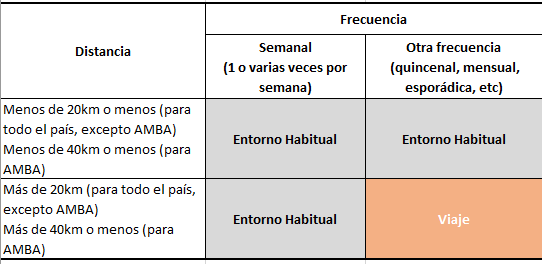
\includegraphics{cuadros_graficos/01_entorno_habitual.png}

\hypertarget{unidades-de-anuxe1lisis}{%
\section{Unidades de análisis}\label{unidades-de-anuxe1lisis}}

El marco conceptual antes definido permite obtener conclusiones a partir de diversas unidades de análisis. A continuación, se las repasan junto con una breve descripción de cada una de ellas:

\begin{enumerate}
\def\labelenumi{\arabic{enumi}.}
\item
  Hogar: es la persona o grupo de personas, parientes o no, que habitan bajo un mismo techo en un régimen de tipo familiar; es decir, comparten sus gastos en alimentación con cargo a un mismo presupuesto.
\item
  Persona: cada uno de los individuos integrantes de un hogar.
\item
  Turista: significa el desplazamiento que realiza una persona fuera del entorno habitual, con una duración inferior al año, pernoctando en el/los lugar/es de destino, por cualquier motivo excepto de ser empleado por una unidad residentes.
\item
  Visita de un día: es el recorrido de una persona fuera del entorno habitual sin pernoctar en el lugar de destino.
\item
  Pernoctación: se trata de una noche de alojamiento de una persona.
\end{enumerate}

\hypertarget{universo-bajo-estudio}{%
\section{Universo bajo estudio}\label{universo-bajo-estudio}}

El universo bajo estudio de la encuesta son los grandes aglomerados urbanos definidos en la EPH del INDEC. Por lo tanto, se consideran 32 aglomerados (para mayor detalle ver el cuadro en el Anexo). Los aglomerados se agrupan en las siguientes Regiones: \footnote{Se debió decidir en qué regiones incluir los aglomerados urbanos ``San Nicolás -- Villa Constitución'' y ``Viedma -- Carmen de Patagones'' puesto que las ciudades se encuentran en distintas provincias y, por ende, en diferentes regiones (según la definición que sigue). Se incluye al primer aglomerado (San Nicolás -- Villa Constitución) en la Región Buenos Aires, mientras que el segundo (Viedma -- Carmen de Patagones), en la Región Patagonia.}

\begin{enumerate}
\def\labelenumi{\arabic{enumi}.}
\item
  Región Ciudad de Buenos Aires.
\item
  Partidos del Conurbano de la Provincia de Buenos Aires.
\item
  Región Interior de la Provincia de Buenos Aires: compuesto por todos los aglomerados pertenecientes a dicha Provincia, excepto Partidos del Conurbano de la Provincia de Buenos Aires.
\item
  Región Córdoba: compuesto por todos los aglomerados pertenecientes a la Provincia de Córdoba.
\item
  Región Litoral: compuesto por todos los aglomerados pertenecientes a las Provincias de Santa Fe, Entre Ríos, Corrientes, Misiones, Formosa y Chaco.
\item
  Región Norte: compuesto por todos los aglomerados pertenecientes a las provincias de Jujuy, Salta, Tucumán, Santiago del Estero, Catamarca y La Rioja.
\item
  Región Cuyo: compuesto por todos los aglomerados pertenecientes a las provincias de Mendoza, San Luis, San Juan.
\item
  Región Patagónica: compuesto por todos los aglomerados pertenecientes a las provincias de La Pampa, Neuquén, Río Negro, Chubut, Santa Cruz y Tierra del Fuego.
\end{enumerate}

A continuación, se presenta un mapa que, a modo ilustrativo, indica los aglomerados que son relevados:

{[}AGREGAR{]} \textbf{Mapa con los aglomerados capitales de provincia o aglomerados urbanos de más de 100.000 habitantes del universo bajo estudio}

\hypertarget{diseuxf1o-muestral}{%
\section{Diseño muestral}\label{diseuxf1o-muestral}}

El diseño muestral a considerar durante el relevamiento de la EVyTH se estructura en las siguientes pautas:

\begin{enumerate}
\def\labelenumi{\arabic{enumi}.}
\item
  Cada una de las regiones definidas es considerada como estrato y se seleccionan muestras independientes en cada uno de ellos.
\item
  El método de selección implementado es el sistemático.
\item
  Cada región, se ordena por Aglomerado -- Partido/Departamento -- Localidad -- Característica Telefónica.
\end{enumerate}

\hypertarget{tamauxf1o-muestral-y-manejo-de-los-reemplazos}{%
\section{Tamaño muestral y manejo de los reemplazos}\label{tamauxf1o-muestral-y-manejo-de-los-reemplazos}}

El tamaño de muestra mensual titular de 2.600 hogares distribuidos a lo largo de cada Región - Aglomerado -- Partido/Departamento - Localidad. Asimismo, en caso de que la muestra titular no pueda ser completada (por ausencia de respondentes, rechazo a responder la encuesta o errores del marco), se seleccionan, con el mismo diseño muestral reemplazos para el hogar titular. Los reemplazos coinciden en la Región, Aglomerado, Partido/Departamento y Localidad y son utilizados luego de, al menos, seis intentos de comunicación insatisfactorios con la muestra inicial.

De esta forma, con el mecanismo de períodos de referencia y ventanas de observación implementados se logra que, para la ventana de observación de un mes determinado, se duplique el tamaño de muestra (se relevan 5.200 hogares).

\hypertarget{marco-de-muestreo}{%
\section{Marco de muestreo}\label{marco-de-muestreo}}

La EVyTH se instrumenta a través de un sistema C.A.T.I. (Computer Assisted Telephone Interviewing). Para ello, se utiliza como marco de muestreo la Guía Telefónica Nacional (GTN) del año 2011 (actualizada anualmente). La encuesta cuenta con una Guía ya consistida y validada.

La GTN está compuesta por los siguientes campos:

\begin{enumerate}
\def\labelenumi{\arabic{enumi}.}
\item
  Rubro/Actividad
\item
  Apellido y Nombre
\item
  Domicilio
\item
  Teléfono
\item
  CP
\item
  Ciudad
\item
  Localidad
\item
  Provincia
\end{enumerate}

\hypertarget{periodicidad-ventana-de-observaciuxf3n-y-peruxedodo-de-referencia}{%
\section{Periodicidad, ventana de observación y período de referencia}\label{periodicidad-ventana-de-observaciuxf3n-y-peruxedodo-de-referencia}}

Para llevar adelante el campo de la EVyTH, se utiliza una periodicidad de muestreo mensual; es decir, todos los meses se releva una muestra seleccionada de acuerdo a la metodología descripta anteriormente.

Además, se contempla una ventana de observación \footnote{El período para el cual se brinda información se denomina ventana de observación.} bimestral para los meses a ser relevados, es decir, períodos de recordación de dos meses consecutivos. Las ventanas de observación de períodos cortos, como este caso, eliminan la necesidad de recordación por tiempos prolongados, lo que favorece la veracidad de la información.

Para dar mayor detalle del mecanismo de ventanas de observación y solapamiento implementado, se presenta el siguiente esquema:

{[}AGREGAR{]} \textbf{Cuadro 2: Periodicidad, Ventana de Observación y Períodos de Referencia}

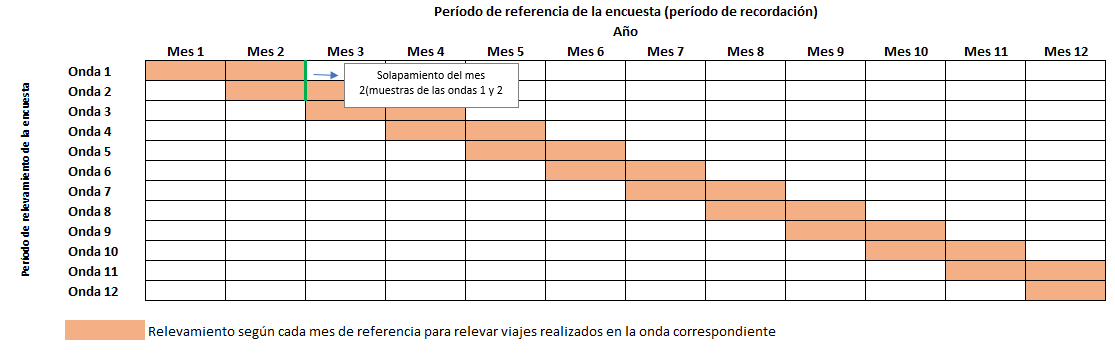
\includegraphics{cuadros_graficos/03_periodo_de_referencia.png}

La EVyTH se desarrolla ``durante doce ondas consecutivas, a razón de una onda por mes calendario''. El mes calendario de comienzo del relevamiento es marzo. Por lo tanto, para ese mes (que sería la Onda 1 de la EVyTH), se encuesta la muestra (titular) de 2.600 hogares (con los remplazos que hicieran falta) y se consulta por los períodos de referencia correspondiente a los dos meses calendarios anteriores (enero y febrero). Durante el segundo mes de relevamiento, abril (Onda 2), se procede de forma similar para los viajes realizados en los dos meses anteriores (febrero y marzo). Consecuentemente el Mes 2 (abril) la muestra queda ``solapada'', habiéndose encuestado 5.200 hogares para este mes (es decir, luego del segundo mes de relevamiento).

De este modo se garantiza que, las estimaciones contenidas en los informes correspondientes a cada mes en el apartado de Anticipo Mensual son obtenidas a partir de 2.600 encuestas efectivas, mientras que para las estimaciones mensuales finales la muestra queda duplicada a 5.200 (lo que garantiza la robustez del resultado).

\hypertarget{esquema-de-rotaciuxf3n-muestral}{%
\section{Esquema de Rotación muestral}\label{esquema-de-rotaciuxf3n-muestral}}

Con el objetivo de mejorar la comparación interanual de las principales variables relevadas, se renueva periódicamente el conjunto de hogares encuestados (panel de respondentes) \footnote{La forma en que se produce esta renovación se denomina esquema de rotación.}. Conceptualmente, el esquema de rotación de una encuesta tiene incidencia sobre los siguientes aspectos:

\begin{enumerate}
\def\labelenumi{\arabic{enumi}.}
\item
  Precisión de las estimaciones del cambio entre dos períodos diferentes.
\item
  Precisión de las estimaciones obtenidas al agregar muestra.
\item
  Nivel de no respuesta (por cansancio del panel).
\end{enumerate}

El objetivo primordial de la EVyTH es medir la evolución de los viajes que, es sabido, es una variable que presenta una gran estacionalidad. Consecuentemente, la medición de la evolución no se realiza a partir de comparar dos meses consecutivos (excepto algunos meses en particular), sino que anualmente o agregando períodos (estival, invernal, etc.).

Tal como se describió anteriormente, el manejo muestral exige escoger la muestra antes de cada mes de relevamiento de modo tal de obtener muestras independientes, pero solapadas. El esquema de rotación que se implementó consiste en incluir en la muestra del mes 1 del año t, la muestra titular de los hogares respondentes del mismo periodo (mes 1) del año anterior (t-1), no con el objetivo de estudiar el comportamiento de esos hogares en particular, sino de modo tal de hacer que las variaciones interanuales no presenten diferencias extremas. De esta forma se maximiza la precisión en cuanto a los cambios suscitados entre un año y otro. Un sistema de rotación muestral como este, permite evitar el cansancio del panel respondente ya que se repiten los hogares luego de doce meses. De esta manera, se logra una mejor ponderación entre ganancia en precisión (al rotar la muestra) y medición del cambio entre dos períodos (dos años).

Es relevante señalar que durante la EVyTH-12 se llevó a cabo una prueba piloto de esta metodología ``de panel'' entre los meses de abril y mayo (ondas 3 y 4). Los resultados fueron positivos ya que no se encontraron sesgos en las características de los respondentes \footnote{El control consistió en evaluar las características principales de los respondentes de la encuesta durante las primeras cuatro ondas de relevamiento del año 2011 y del año 2012. El objetivo fue estudiar si se producía algún sesgo demográfico al utilizar muestras panel. Los relevamientos de las ondas 3 y 4 (relevamientos de abril y mayo) de la EVyTH-12 fueron panel (incluyeron a los hogares respondentes del mismo periodo del año anterior), mientras que las ondas 1 y 2 (febrero y marzo) no lo fueron. Los resultados del estudio demostraron que no se encontraron variaciones significativas en ningunas de las variables estudiadas (edad promedio edad en tramos, relación de parentesco del miembro respondente con el jefe de hogar, asistencia a establecimiento educativo, máximo nivel educativo alcanzado, situación ocupacional) entre los meses con muestra panel y los meses sin muestra panel.} , a la vez que se aumentó la tasa de efectividad de las encuestas \footnote{Se estudiaron las características de los respondentes no notándose diferencias estadísticamente significativas entre los respondentes que aceptaron ser encuestados el año anterior respecto del mismo grupo que aceptó ser encuestado en el 2012.}. En efecto, en comparación con las ondas en las que no fue implementada esta metodología de panel (es decir, para las ondas 1 a 4 de la EVyTH-11 y ondas 1 y 2 de la EVyTH-12), la tasa de efectividad de encuesta para los hogares titulares durante las ondas en las que sí se adoptó, (es decir, ondas 3 y 4) fue del doble. Mientras que se halló que poco más de dos de cada diez hogares de la muestra titular decidieron responder la encuesta en las primeras ondas, casi cinco de cada diez decidieron hacerlo en las ondas 3 y 4 durante el relevamiento de la EVyTH-12.

Además, se realizó un control por características sociodemográficas del miembro respondente para verificar que no se hubiera sesgado la muestra. Las variables consideradas fueron:

\begin{enumerate}
\def\labelenumi{\arabic{enumi}.}
\item
  edad promedio del miembro respondente
\item
  jefe de hogar o relación de parentesco con el jefe de hogar
\item
  asistencia a establecimiento educativo
\item
  máximo nivel educativo alcanzado
\item
  situación ocupacional
\end{enumerate}

El estudio arrojó el resultado antes comentado: no se encontraron mayores diferencias socio-económicas entre aquellos que accedieron a contestar las preguntas de esta edición de la encuesta con aquellos que lo hicieron en las ondas con distinta metodología.

\hypertarget{consistencia-y-validaciuxf3n}{%
\section{Consistencia y validación}\label{consistencia-y-validaciuxf3n}}

Con el objeto de garantizar la calidad de la información se utiliza un proceso de validación y consistencia de los ficheros resultantes de la encuesta para aplicarse previo a cualquier imputación o tratamiento de información faltante. Dicho proceso se implementa mediante un programa que permite gestionar el proceso de validación y las correspondientes correcciones en los casos de hallar inconsistencias que ha sido diseñado especialmente para la EVyTH.

En este tipo de procesos, el objetivo es controlar los valores o el campo de variación (rango de valores) de cada variable del cuestionario. En una primera etapa, la validación se realiza exclusivamente para cada uno de los individuos registrados, independientemente de su interrelación con la información relevada en otros individuos del mismo hogar. Esto significa que esta validación inicial se realiza en forma independiente para cada individuo y para cada variable del cuestionario.

En las preguntas cerradas se controla que los códigos introducidos se encuentren dentro del rango de valores correspondientes a dicha variable. Por ejemplo, en la variable ``NIVEL DE INSTRUCCIÓN'', sólo deben presentarse los códigos 01 a 10 y el código 99 para el caso de no respuesta.

Una segunda etapa del proceso de validación y consistencia consiste en la validación cruzada de la información contenida entre variables relevadas en un mismo individuo. Es decir, se analizan las interrelaciones lógicas entre dos o más preguntas de un mismo individuo. Por ejemplo, si no responde en la pregunta sobre si trabaja o no, pero luego responde que es ``ama de casa'', entonces debería corresponder la respuesta ``No'' a la pregunta sobre si trabaja.

El proceso de validación también implica el manejo de las encuestas parcialmente completas. Se implementó un criterio para determinar cuáles encuestas no pueden ser utilizadas para extraer información y cuáles si, de forma tal de minimizar la pérdida de datos. Se considera una encuesta válida cuando el respondente haya contestado todas las preguntas referidas al comportamiento turístico del hogar dentro del periodo de referencia correspondiente y, al menos, haya respondido sobre las características básicas del jefe (sexo, edad, nivel educativo). Si bien la gran mayoría de los entrevistados responden hasta el final de la encuesta (y, por ende, se cuenta con las características de cada una de las personas que integran el hogar), en algunas ocasiones el respondente se niega a suministrar información personal. Como se mencionó, en estos casos el criterio para dar por válida una encuesta es que al menos se haya obtenido la información básica sobre el jefe. En base a la información recolectada hasta allí (cantidad de integrantes, características del jefe, observaciones del encuestador sobre el sexo y/o la edad de las personas restantes -información que suele surgir durante el desarrollo de la entrevista), se procede a imputar las características básicas de las personas del hogar faltantes.

Por último, existe un proceso de validación ``ex -- post''. Este mecanismo consiste en estudiar cada una de las variables discriminadas en función de distintos cortes (etarios, regionales, etc.) con el fin de analizar respuestas que se ubiquen fuera de los rangos definidos como ``normales''.

\hypertarget{procedimiento-de-imputaciuxf3n}{%
\section{Procedimiento de imputación}\label{procedimiento-de-imputaciuxf3n}}

Una vez finalizada la etapa de validación y consistencia de la información comienzan las tareas de imputación de la falta de respuesta en las variables de cada base de datos. En la sección a continuación se realiza una breve descripción del proceso de imputación de las principales variables relevadas por la EVyTH: ingreso total del hogar y gasto del viaje.

Desde el punto de vista conceptual, el método de imputación que se utiliza, al sustituir valores perdidos, requiere que la imputación no modifique las características de la variable en estudio. Por este motivo es recomendable demostrar, luego de la imputación, que no se han generado cambios relevantes en la distribución de la variable imputada.

En una primera instancia se procede a estudiar y evaluar la imputación de las variables ``Ingreso Total del Hogar'' y ``Gasto en Viajes'', sin embargo, lo aplicado en esta situación es empleado en otras variables de interés (por ejemplo, edad, sexo y situación laboral).

Para el caso de la variable Ingreso Total del Hogar, considerando que se trata de una variable categórica ordinal, para su imputación se utiliza un modelo de Regresión Logística Politómica con Variable Respuesta Ordinal.

Para el caso de la imputación de la variable ``Gasto del Viaje'', al ser una variable continua (no está categorizada), la metodología implementada para su imputación sigue un modelo de regresión en dos etapas puesto que debe contemplarse que la variable ingreso es una variable con distribución marcadamente sesgada (por lo que una técnica que asuma una distribución Normal no debería ser adecuada sin una previa transformación que asegure dicho supuesto). Esta metodología busca, en la primera etapa, ``colocar'' el valor del gasto faltante en una categoría de gasto, en función de los valores observados en las variables explicativas mientras que, en la segunda etapa, se selecciona un valor de esa categoría para ``asignar'' al registro. Por otra parte, entre las variables explicativas que se tomaron en cuenta para su imputación se encuentran: distancia recorrida, cantidad de noches, cantidad de miembros del hogar, tipo de alojamiento, medio de transporte utilizado, motivo del viaje, tiempo de organización del viaje, mes en que se realizó el viaje, entre otras.

\hypertarget{proceso-de-calibraciuxf3n}{%
\section{Proceso de calibración}\label{proceso-de-calibraciuxf3n}}

Una etapa crítica en toda encuesta por muestreo es la expansión de la información. Una selección adecuada, y el posterior desarrollo, de una metodología para ponderar los datos muestrales es importante, ya que debe atender simultáneamente varias necesidades. Las distintas temáticas estudiadas, y la necesidad de lograr estimaciones adecuadas para cada una de ellas, obliga a que ésta sea lo más eficiente posible, en términos de precisión, cuidando no privilegiar a algunas en perjuicio de otras. Al mismo tiempo, su implementación debe ser simple, flexible y económica en tiempos de ejecución y cálculo.

Uno de los problemas más comunes en las encuestas complejas de gran envergadura es que una vez desarrollado el trabajo de campo existen algunos subgrupos de la población objetivos sub o sobre-representados.

Esta dificultad lleva a que los sesgos puedan ser importantes, impidiendo una interpretación correcta de las estimaciones o imposibilitando la comparación de los resultados con fuentes alternativas.

Para corregir esto, en la práctica es habitual corregir los pesos o factores de expansión iniciales (las inversas de las probabilidades de inclusión) con la ayuda de información auxiliar. El hecho de contar con dicha información auxiliar en la etapa de estimación permite el empleo de estimadores que la involucran. Dentro de este tipo de estimadores están los que se obtienen a través de los métodos de calibración. Éstos, en su forma más general, tienen como objetivo crear nuevos pesos que resultan de modificar o calibrar las ponderaciones iniciales por diseño.

El empleo adecuado de la técnica de calibración permite:

\begin{enumerate}
\def\labelenumi{\arabic{enumi}.}
\item
  Reducir el error cuadrático medio de las estimaciones.
\item
  Corregir posibles sesgos en la etapa de selección.
\item
  Dar una solución al problema de ``no-respuesta''.
\item
  Lograr, a partir de las restricciones impuestas, una deseable consistencia, o concordancia, entre los totales conocidos y los obtenidos a través de la muestra, de las variables auxiliares.
\end{enumerate}

La calibración consiste básicamente en la resolución de un problema de minimización numérica. Dicho problema queda planteado con la elección de una distancia, entre los nuevos ponderadores y los originales, y la utilización de un conjunto de restricciones impuestas sobre las variables auxiliares que intervienen en el ajuste.

Para el presente trabajo se utiliza y adapta la macro CALMAR \footnote{El algoritmo del Calmar a utilizar durante la calibración puede ser consultado en: \url{http://www.restore.ac.uk/PEAS/saspackage.php}}, escrita en lenguaje SAS por Sautory (1991), la cual calcula los pesos calibrados cuando la información auxiliar de una encuesta consiste de totales marginales conocidos dispuestos en una tabla de frecuencias de dimensiones arbitrarias. La macro mencionada trabaja con cuatro funciones, de las cuales para la EVyTH se trabaja sólo con tres. A continuación, se brinda una pequeña descripción de cada una de ellas.

\begin{enumerate}
\def\labelenumi{\arabic{enumi}.}
\item
  Método Lineal: knitr::include\_graphics(``salidas/tabla1.png'')
\item
  Método multiplicativo (o método ranking): knitr::include\_graphics(``salidas/tabla1.png'')
\item
  Método logit: Fijar dos constantes L y U, tal que L\textless1\textless U, y sea knitr::include\_graphics(``salidas/tabla1.png'') . Luego knitr::include\_graphics(``salidas/tabla1.png'')
\end{enumerate}

{[}AGREGAR{]} fórmulas en markdown

si L\textless x\textless U, y knitr::include\_graphics(``salidas/tabla1.png'') en otro caso. La función F correspondiente es:
knitr::include\_graphics(``salidas/tabla1.png'')

que toma valores entre L y U

La función logit descripta en el punto 3. constituye una función inusual que surge del deseo de restringir el rango de los nuevos pesos wk para evitar los pesos extremos, los cuales pueden ser eliminados a través de una apropiada elección de L y U.

Para el proceso de calibración de la EVyTH se intenta, no siempre con éxito (de acuerdo con nuestra experiencia en las ediciones de la EVyTH anteriores), utilizar el método 1), dado que el proceso iterativo solamente involucra un paso. La dificultad que posee este método es que, en muchos casos y debido a la estructura interna de la muestra con respecto a las variables de calibración, brinda pesos negativos los cuales obviamente no tienen sentido dentro del muestreo. Es por ello que para aquellas Regiones donde se encuentran estas dificultades, se aplica el método 2., el cual posee la ventaja de evitar los pesos negativos.

El método 3. se aplica en aquellas Regiones donde los nuevos pesos calculados por el método 1. o 2. resulten extremos. Se intenta, en la mayoría de las Regiones, que los pesos resultantes cumplan con la siguiente condición: knitr::include\_graphics(``salidas/tabla1.png'') , necesitando en algunas Regiones ampliar dichos márgenes.

Se realiza la calibración en forma independiente en cada Región dado que las muestras son independientes y además se brinda estimaciones de cada una de ellas.

Con respecto a la información auxiliar empleada para la calibración y el ajuste de las estructuras internas de la muestra, se recurrió a proyecciones de población en base al INDEC. Se tiene en cuenta los siguientes totales a nivel de cada una de las siete Regiones:

\begin{enumerate}
\def\labelenumi{\arabic{enumi}.}
\item
  Total de personas por sexo.
\item
  Total de personas por grupos de edad.
\item
  Total de personas por nivel educativo.
\item
  Total de viviendas.
\end{enumerate}

Los grupos de edad están compuestos de la siguiente manera:

\begin{enumerate}
\def\labelenumi{\arabic{enumi}.}
\item
  0 -- 17 años,
\item
  18 -- 34 años,
\item
  35 -- 54 años, y
\item
  mayores de 55 años.
\end{enumerate}

Nivel Educativo está conformado por cuatro grupos siendo los mismos:

\begin{enumerate}
\def\labelenumi{\arabic{enumi}.}
\item
  Sin Instrucción/Hasta Primario Incompleto,
\item
  Primario Completo/Secundario Incompleto,
\item
  Secundario Completo/Terciario Incompleto/Universitario Incompleto, y
\item
  Terciario Completo/Universitario Completo/Posgrado/Maestría/Doctorado
\end{enumerate}

Importa aclarar que los Totales de Población y Viviendas utilizados en la calibración se obtienen de Proyecciones elaboradas por INDEC, las cuales actualiza a medida que se dispone de la información del Censo Nacional de Población, Hogares y Viviendas desarrollado en el 2010.

Por otra parte, para cada uno de los meses de relevamiento, se realizan 2 calibraciones. Una calibración, inmediatamente al final del relevamiento con el objetivo de dar el anticipo nacional de las principales estimaciones de interés correspondiente a los viajes realizados durante el mes anterior al de relevamiento. La segunda calibración se realiza al final del bimestre donde se dan todas las estimaciones definitivas a nivel regional para el mes que haya duplicado la muestra (5.200 encuestas). Es decir, si el mes de relevamiento fuera enero, por ejemplo, se consulta por los viajes realizados (que finalizaron) en el mes de diciembre y noviembre (1 y 2 meses atrás del mes de relevamiento). Al final del relevamiento de ese mes (enero) se brinda un anticipo nacional para el mes de diciembre con un tamaño de muestra de 2.600 hogares. Luego, durante el próximo mes de relevamiento (febrero), el período de referencia serán los meses de diciembre y enero, por lo que, al finalizar, producto del solapamiento descripto anteriormente, se relevan 5.200 hogares para el mes de diciembre (2.600 durante el relevamiento de enero y 2.600 casos durante el relevamiento de febrero). Por lo tanto, al finalizar el relevamiento de febrero se brinda una estimación definitiva con nivel de desagregación geográfica regional para el mes de diciembre y un anticipo nacional (con 2.600 casos) para el período de referencia de enero.

Es preciso aclarar que tanto la calibración correspondiente al anticipo (con representatividad nacional) y definitiva (con desagregación por región) de cada uno de los meses, se realiza en forma independiente en cada una de las Regiones. Por lo tanto, la calibración del anticipo se lleva a cabo en cada una de las regiones, brindándose resultados nacionales, y luego, al mes siguiente, se vuelve a realizar una calibración en cada región con el total de la muestra definitiva (para lo que no se consideran los ponderadores estimados durante el anticipo).

Para salvar posibles inconsistencias en los cuadros a publicar, los pesos calibrados son tratados por un algoritmo de redondeo para eliminar la componente decimal con los que salen del proceso iterativo sin destruir las concordancias alcanzadas.

\hypertarget{coeficientes-de-variaciuxf3n}{%
\section{Coeficientes de variación}\label{coeficientes-de-variaciuxf3n}}

La metodología de la EVyTH-13 incorporó el cálculo de estadísticos (o indicadores) con la finalidad de brindarle al usuario de los datos una medida del grado de precisión de las estimaciones calculadas para cada uno de los informes de resultados. Esto es especialmente relevante con el fin de brindarle al lector noción sobre cuán preciso es el estimador que se utiliza (o cita) de forma tal que este pueda medir los ``riesgos'' que ello implique.

Desde la perspectiva del diseño muestral la EVyTH se encuadra dentro de los diseños estratificados con selección sistemática dentro de cada uno de los estratos (ocho estratos en total siendo estos las Regiones del Ministerio de Turismo, Capital Federal, Partidos Gran Buenos Aires, Resto Pcia. Buenos Aires, Córdoba, Litoral, Norte, Cuyo, Patagonia). Si bien el método de selección sistemática es recomendable y eficiente para muestras telefónicas, su uso implica que no exista estimadores no sesgados de varianza. Para sortear esta dificultad a la hora del cálculo de los errores muestrales se propuso plantear el supuesto de que la población está en ``orden aleatoria''. Bajo este supuesto se pueden utilizar los estimadores de un muestreo estratificado con selección simple al azar. Con esto se resuelve el problema de cómo estimar los desvíos estándares de cada estimador.

En el caso particular de la EVyTH, los informes presentaron el cálculo de los CV para cada estimador relevante (según el informe que se trate), aclarándose para aquellos que presenten un CV superior al 30\% que ``el resultado debe considerase a título indicativo puesto que la estimación no presenta el mínimo de precisión preestablecido''.

Además de los CV, en los distintos informes producidos a partir del relevamiento de la EVyTH, se calculan intervalos de confianza puesto que facilitan la comprensión acerca del grado de precisión de los distintos estimadores calculados para aquellos lectores no instruidos en el tema.

El Cuadro a continuación destalla los Coeficientes de Variación que son calculados según cada informe producido en el marco de la encuesta.

{[}AGREGAR{]} \textbf{Cuadro 3: Coeficientes de Variación calculados según cada Informe de la EVyTH}

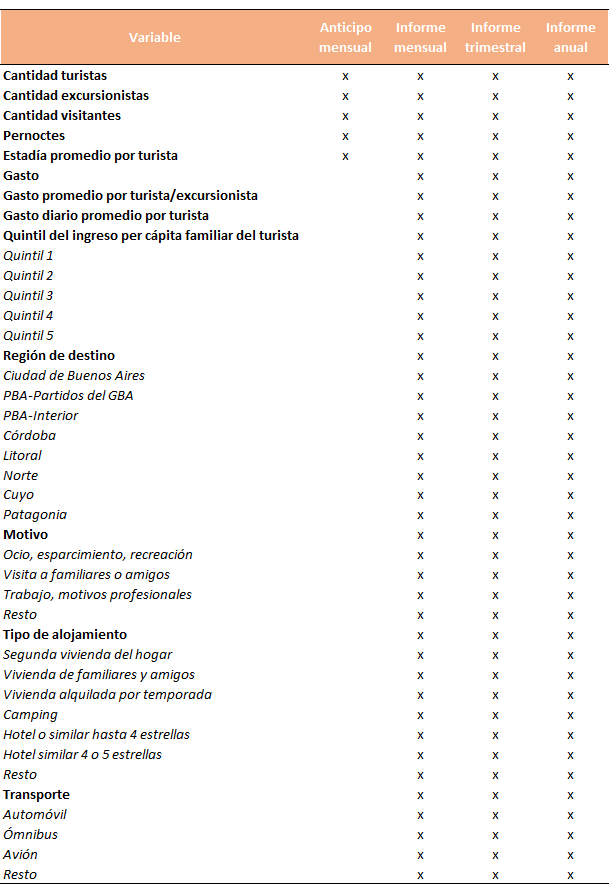
\includegraphics{cuadros_graficos/04_coeficiente_de_variacion.png}

Para comprender fácilmente la forma en que se implementó la metodología descripta anteriormente, se brindan a continuación algunos ejemplos de estimaciones de CV.

{[}AGREGAR{]} \textbf{Cuadro 4: Análisis de margen de error para informes de adelanto y final. Resultados básicos para agosto 2013}

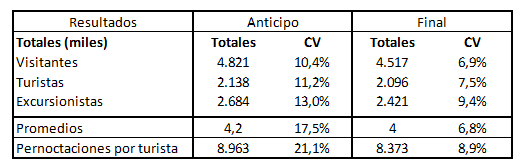
\includegraphics{cuadros_graficos/05_analisis_margen_de_error.png}

{[}AGREGAR{]} \textbf{Gráfico 2: Análisis de margen de error para informes de adelanto y final. Visitantes (intervalo de confianza al 90\%). Resultados para agosto 2013.}

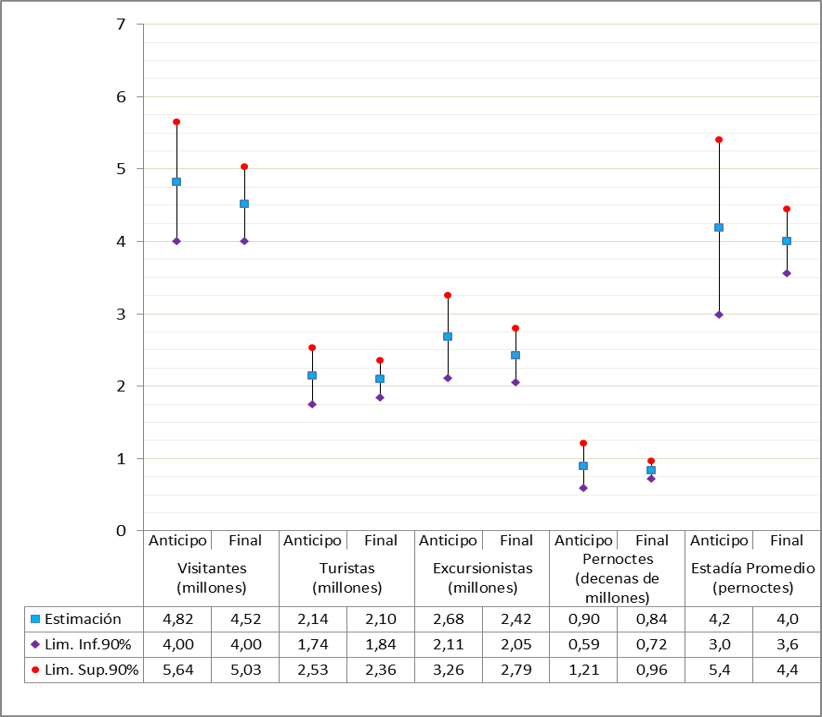
\includegraphics{cuadros_graficos/06_grafico_margen_de_error.png}

\hypertarget{cuestionario}{%
\chapter{Cuestionario}\label{cuestionario}}

A continuación, se expone el Cuestionario que se implementó en la EVyTH.
El mismo consiste en un Cuestionario Base (o sección ``pétrea'') que, básicamente, pretende relevar los viajes realizados en los últimos dos meses y un Cuestionario ``ad-hoc'' que tiene la función de captar eventuales viajes futuros para fechas especiales como son los periodos de Verano/Invierno.

\hypertarget{antecedente-de-la-actual-ediciuxf3n-de-la-evyth}{%
\section{Antecedente de la actual edición de la EVyTH}\label{antecedente-de-la-actual-ediciuxf3n-de-la-evyth}}

El Cuestionario implementado en la EVyTH-06, constituyó el modelo sobre el cual se trabajó para llegar al cuestionario aplicado en la Prueba Piloto, en la EVyTH telefónica de los años 2012 en adelante.
Al observarse el Formulario, se puede notar que la estructura conceptual del cuestionario ha perdurado desde su comienzo, sin embargo, seguramente fue preciso realizar algunas modificaciones atendiendo a situaciones de diversa índole \footnote{Circunstancias a las que se le debe adicionar el hecho de que ahora el relevamiento es telefónico (a diferencia de la EVyTH-06, que se realizó cara a cara).} .
Los cambios que ha sufrido el cuestionario se resumen a continuación y resultan en el Formulario Base anexado a este informe \footnote{Este Formulario Base ya incorpora la actualización de los tramos de gastos (según tipo de viaje) y de ingreso (así como también los cambios necesarios a las preguntas de comportamiento turístico).}.

\hypertarget{descripciuxf3n-del-formulario}{%
\section{Descripción del formulario}\label{descripciuxf3n-del-formulario}}

En la presente sección, se describe el cuestionario, que se utiliza para la presente edición de la EVyTH.
Este puede ser dividido en dos grandes secciones: un bloque ``pétreo'' (cuyo contenido solo esporádicamente sufre alguna alteración menor) y otro bloque conformado por preguntas que cambian en función de relevamientos ``ad-hoc'' que resultan de interés según el período y la ocasión.
Si bien esta sección es utilizada para indagar sobre la expectativa que los encuestados tienen en relación a la posibilidad de realizar algún viaje en un momento futuro (como los períodos de alta estacionalidad turística), puede ser utilizada, también, para llevar adelante encuestas de opinión u de otra índole \footnote{Su característica básica es que es completamente flexible permitiendo realizar relevamientos ``ad-hoc'' de forma fácil.} (durante la EVyTH-20 se indago sobre los perjuicios que tuvo la pandemia a causa del virus COVID-19 y sobre futuros viajes pos pandemia).

\hypertarget{cuestionario-base-secciuxf3n-puxe9trea}{%
\subsection{Cuestionario base (sección ``pétrea'')}\label{cuestionario-base-secciuxf3n-puxe9trea}}

Como se indicó anteriormente, la sección del cuestionario que se describe a continuación prácticamente no ha sufrido alteraciones desde el comienzo de la primera edición de la EVyTH.
La idea es minimizar los cambios de contenido a esta parte del cuestionario con el fin de lograr la mayor compatibilidad entre los datos relevados en distintos momentos del tiempo y, de esta forma, generar una serie de tiempo lo más extensa posible.

Esta sección se compone de 9 Bloques; a saber:

\begin{itemize}
\tightlist
\item
  Bloque ``Características de los miembros del hogar''.
\end{itemize}

Este bloque está subdivido en tres.
(i) Al inicio de la encuesta, sólo se indaga por la cantidad de personas que integran el hogar y las iniciales (de forma tal de mantener el anonimato) de cada uno de los miembros del hogar.
(ii) Al final del cuestionario, luego de indagar por la realización de viajes y visitas y sus características, se indaga por las características de los miembros del hogar, bajo el supuesto de que, con el devenir de la encuesta, el entrevistado gana confianza y se muestra menos renuente a responder estas preguntas.
En este mismo sub-bloque se indaga por el comportamiento turístico en el año calendario anterior a la encuesta \footnote{Este aspecto se indaga durante los meses de febrero hasta mayo inclusive.}; (iii) La indagación por los ingresos totales del hogar, que cierra la encuesta, se incluye como otro sub-bloque también al finalizar el Formulario Base.

\begin{itemize}
\item
  Bloque ``Segundas Viviendas''.
  Se indaga únicamente por las segundas viviendas que el hogar dispuso y utilizó durante el periodo de referencia.
\item
  Bloque ``Viajes de corta duración a segundas viviendas'': 1 a 3 noches (VCDS).
\item
  Bloque ``Viajes de larga duración a segundas viviendas'': 4 noches o más (LDSV).
\item
  Bloque ``Visitas de un día a segundas viviendas'' (VDSV).
\item
  Bloque ``Viajes no reiterados en Argentina'' (VA).
\item
  Bloque ``Viajes no reiterados al exterior'' (VE).
\item
  Bloque ``Viajes a destinos reiterados'' (DR).
\end{itemize}

Este bloque funciona como ``reserva'', es decir, no se pregunta directamente al entrevistado si realizaron viajes de este tipo, sino que el encuestador lo completa en caso de detectar la existencia de este tipo de viajes en la indagación de los bloques anteriores (VA y VE).

\begin{itemize}
\item
  Bloque ``Visitas de un día''.
\item
  Bloque sobre viaje en períodos turísticos especiales.
\end{itemize}

Este relevamiento complementario indaga por la posibilidad de que alguno de los miembros del hogar haya realizado viajes en la/s fecha/s especiales durante los meses de referencia (por ejemplo, períodos de temporada de verano/invierno). Es un bloque del cuestionario base que se ``activa'' automáticamente cuando, en los meses de referencia, ha habido un fin de semana largo. En función de ello, se consulta explícitamente si el encuestado ha viajado durante ese momento específico del mes.

\begin{itemize}
\tightlist
\item
  Comportamiento turístico de las personas.
\end{itemize}

Finalmente, el formulario también incorpora, solo durante los meses de febrero a mayo, una sección donde se indaga por viajes realizados durante al año anterior a modo de conocer el comportamiento turístico de las personas.
Con la información recabada en esta sección se confecciona el informe sobre Comportamiento Turístico de las Personas Sinópticamente, la lógica del Formulario Base puede resumirse a través del siguiente cuadro:

\textbf{Cuadro 5: Esquematización del Cuestionario utilizado durante la EVyTH}

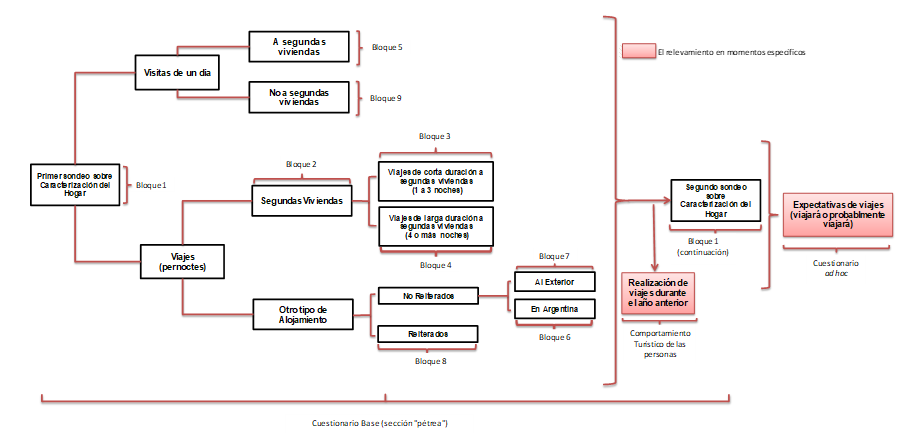
\includegraphics{cuadros_graficos/07_esquema_cuestionario.png}

El cuestionario base contiene su propia terminología para caracterizar a los viajes (en sentido amplio).

Así, por ejemplo, cuando el visitante pernocta al menos una noche en el lugar de destino, se especifica como ``viajes'' y ``viajeros'' propiamente dichos. Cuando la persona no pernocta en el lugar de destino, se hace referencia a ``visitas de un día'' y ``visitantes'' o ``excursionistas''. Por lo tanto, en función de una serie de variables, se han definido diferentes tipos de viajes.

Estas variables son:

\begin{enumerate}
\def\labelenumi{\arabic{enumi}.}
\item
  \textbf{Cantidad de noches en el lugar visitado.} Se consideran las noches pasadas en alojamientos del lugar visitado.
\item
  \textbf{Tipos de Alojamiento donde pernoctaron.} Se clasifican en dos grupos:
\end{enumerate}

\begin{verbatim}
- "Segundas viviendas" 

- "Otros tipos de alojamientos": aquí se incluyen todos los tipos de alojamiento diferentes a las segundas viviendas (hoteles de todas las categorías, camping, casas de familiares o amigos, viviendas alquiladas por temporadas, etc.).
\end{verbatim}

\begin{enumerate}
\def\labelenumi{\arabic{enumi}.}
\tightlist
\item
  \textbf{Ubicación del Destino Principal}, según sea:
\end{enumerate}

\begin{verbatim}
- En Argentina (ciudad/localidad).

- En otro país.
\end{verbatim}

\begin{enumerate}
\def\labelenumi{\arabic{enumi}.}
\tightlist
\item
  Viajes Similares en los últimos 2 meses. De acuerdo a la cantidad de viajes realizados a un mismo destino con características similares (miembros participantes, cantidad de noches, tipo de alojamiento, motivo principal, etc.) los viajes se clasifican en:
\end{enumerate}

\begin{verbatim}
- "Reiterados": cuando hayan realizado 3 o más viajes en los últimos 2 meses.

- "No reiterados": cuando se hayan realizado uno o dos viajes en los últimos 2 meses.
\end{verbatim}

La información que se solicita depende del tipo de viaje que se trate y se registra en un Bloque específico del Formulario Base. Esta clasificación responde a la estrategia definida para mejorar la indagación y captación de los distintos viajes que las personas pueden realizar. En función de las variables mencionadas, llegamos a la siguiente clasificación:

\textbf{Cuadro 6: Caracterización de los viajes a ser relevados y ubicación en el formulario base}

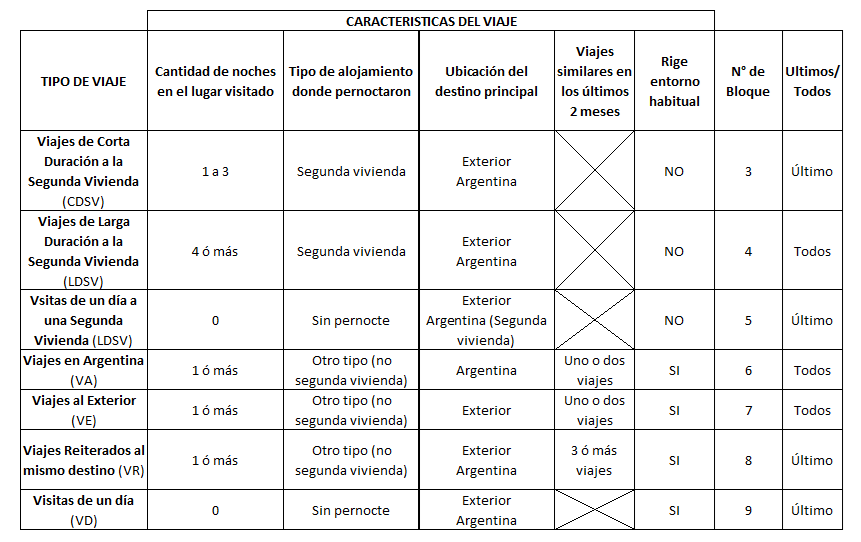
\includegraphics{cuadros_graficos/08_caracterizacion_de_los_viajes.png}

En la última columna del cuadro precedente se señalan dos situaciones: (a) en ciertos tipos de viajes (CDSV, VDSV, VR, VD), dentro de cada bloque, se indaga por la cantidad de viajes o visitas realizadas a cada lugar visitado y luego se realizan algunas preguntas sobre el último de los viajes o visitas a cada lugar; (b) en otros tipos de viajes (LDSV, VA, VE) se consulta directamente por cada uno de los viajes realizados. Esto es así porque por la propia definición de los tipos de viaje que componen el primer grupo se trata de viajes muy parecidos entre sí; en cambio, en el segundo grupo, los viajes englobados dentro de un mismo tipo pueden ser totalmente distintos.

Excepto algún caso particular, existe un núcleo de preguntas que no varía según el tipo de viaje realizado por el hogar. Por ejemplo, se consulta por destino, tipo de alojamiento, actividades, etc.

\hypertarget{estructura-del-cuestionario-base}{%
\subsection{\texorpdfstring{\textbf{ESTRUCTURA DEL CUESTIONARIO BASE}}{ESTRUCTURA DEL CUESTIONARIO BASE}}\label{estructura-del-cuestionario-base}}

Con el fin de brindar una descripción resumida del Formulario Base, se presenta su estructura y las variables relevadas.

\textbf{Cuadro 7: Estrucura del Formulario Base según tipo de pregunta para cada viaje}

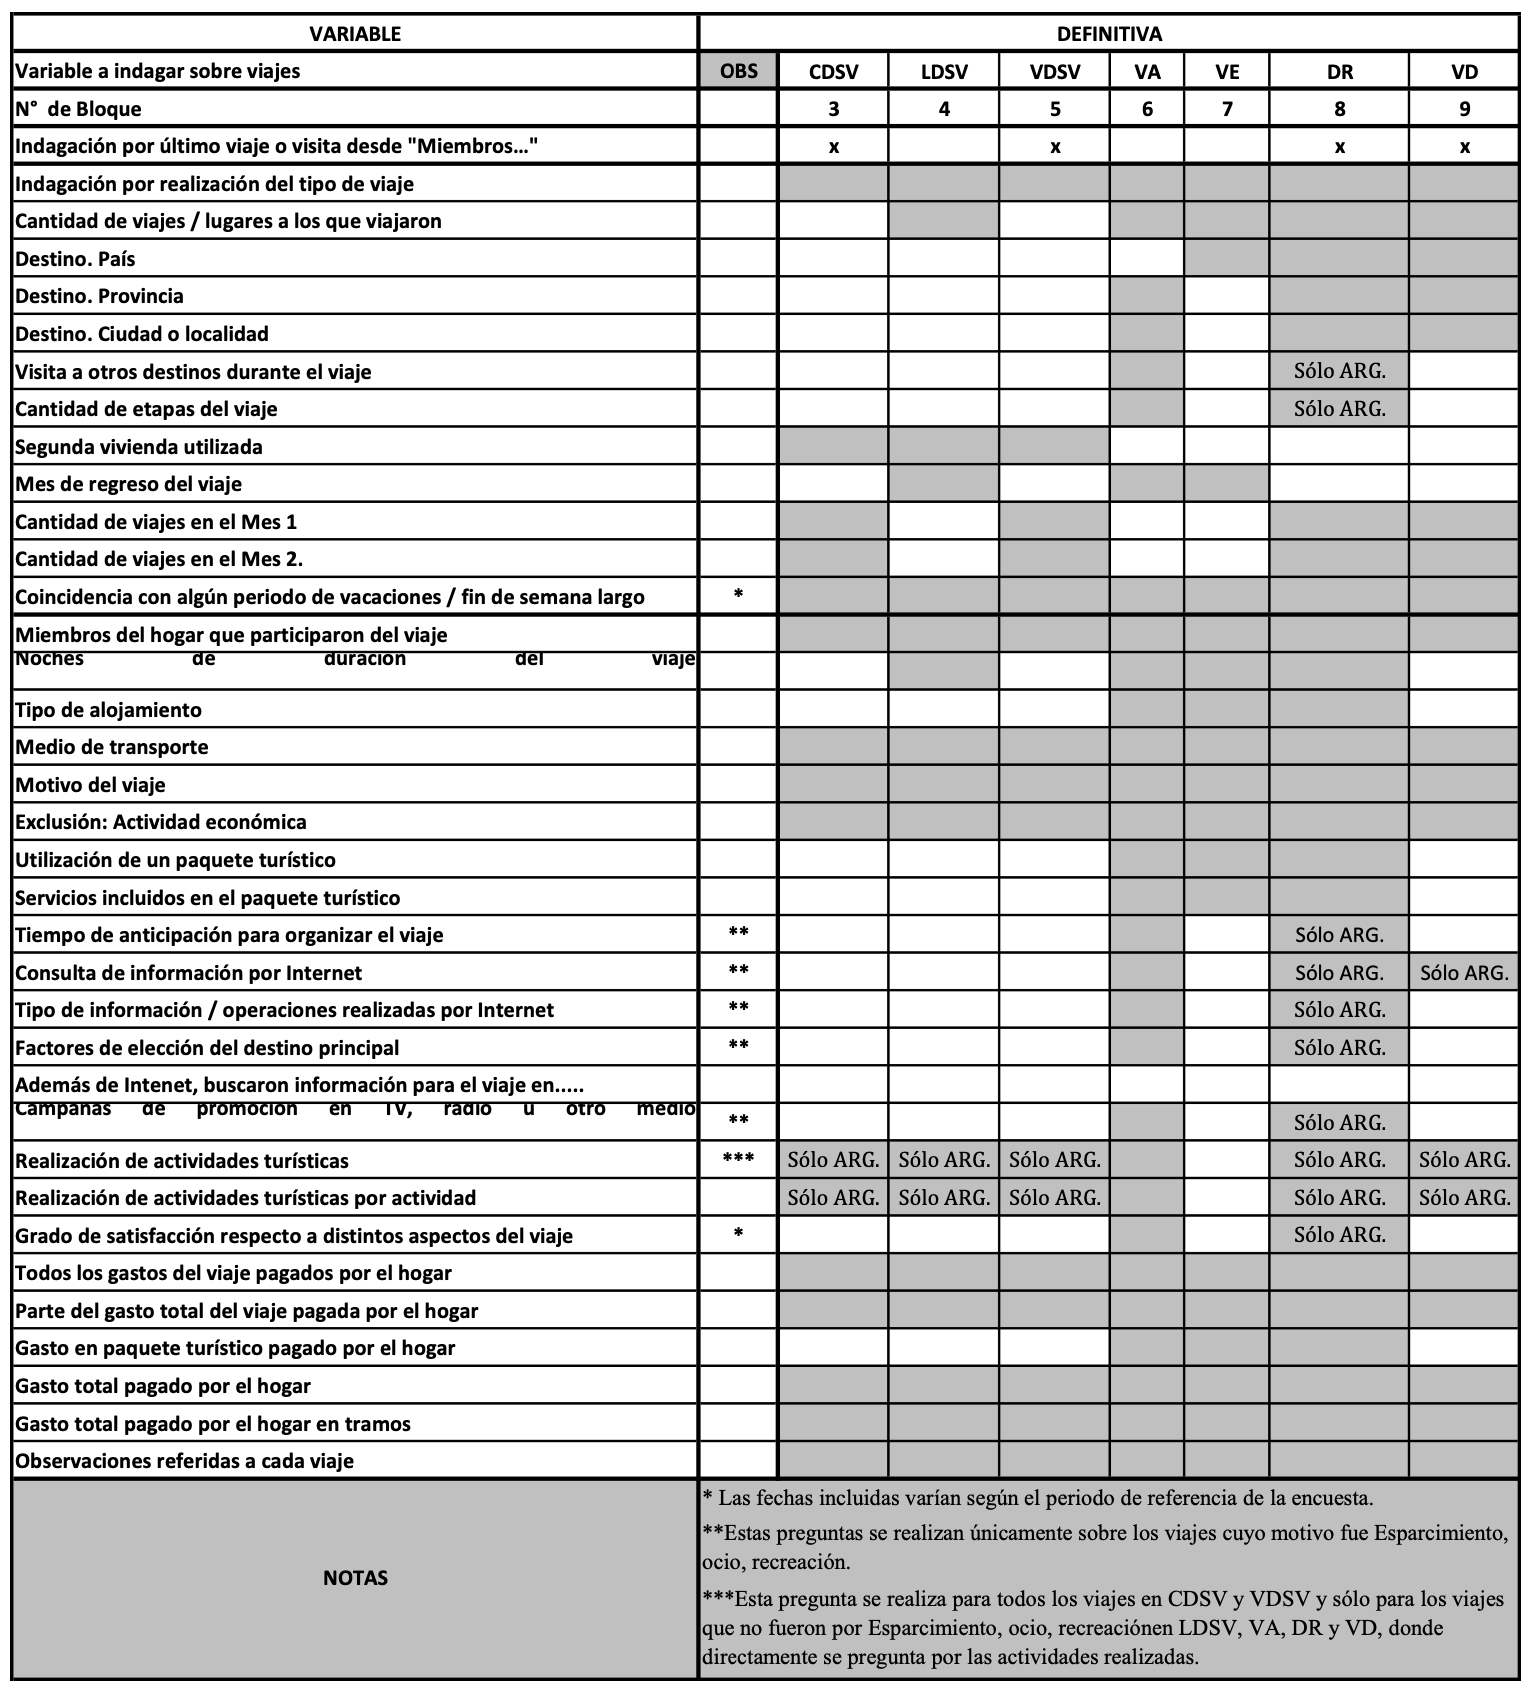
\includegraphics{cuadros_graficos/09_estructura_del_formulario.png}

\hypertarget{anexo}{%
\chapter{Anexo}\label{anexo}}

\hypertarget{composiciuxf3n-de-los-aglomerados}{%
\section{Composición de los aglomerados}\label{composiciuxf3n-de-los-aglomerados}}

A continuación, se describen los 32 aglomerados que se considerarán para estratificar la muestra.

\textbf{Cuadro 22: Composición de Aglomerados}

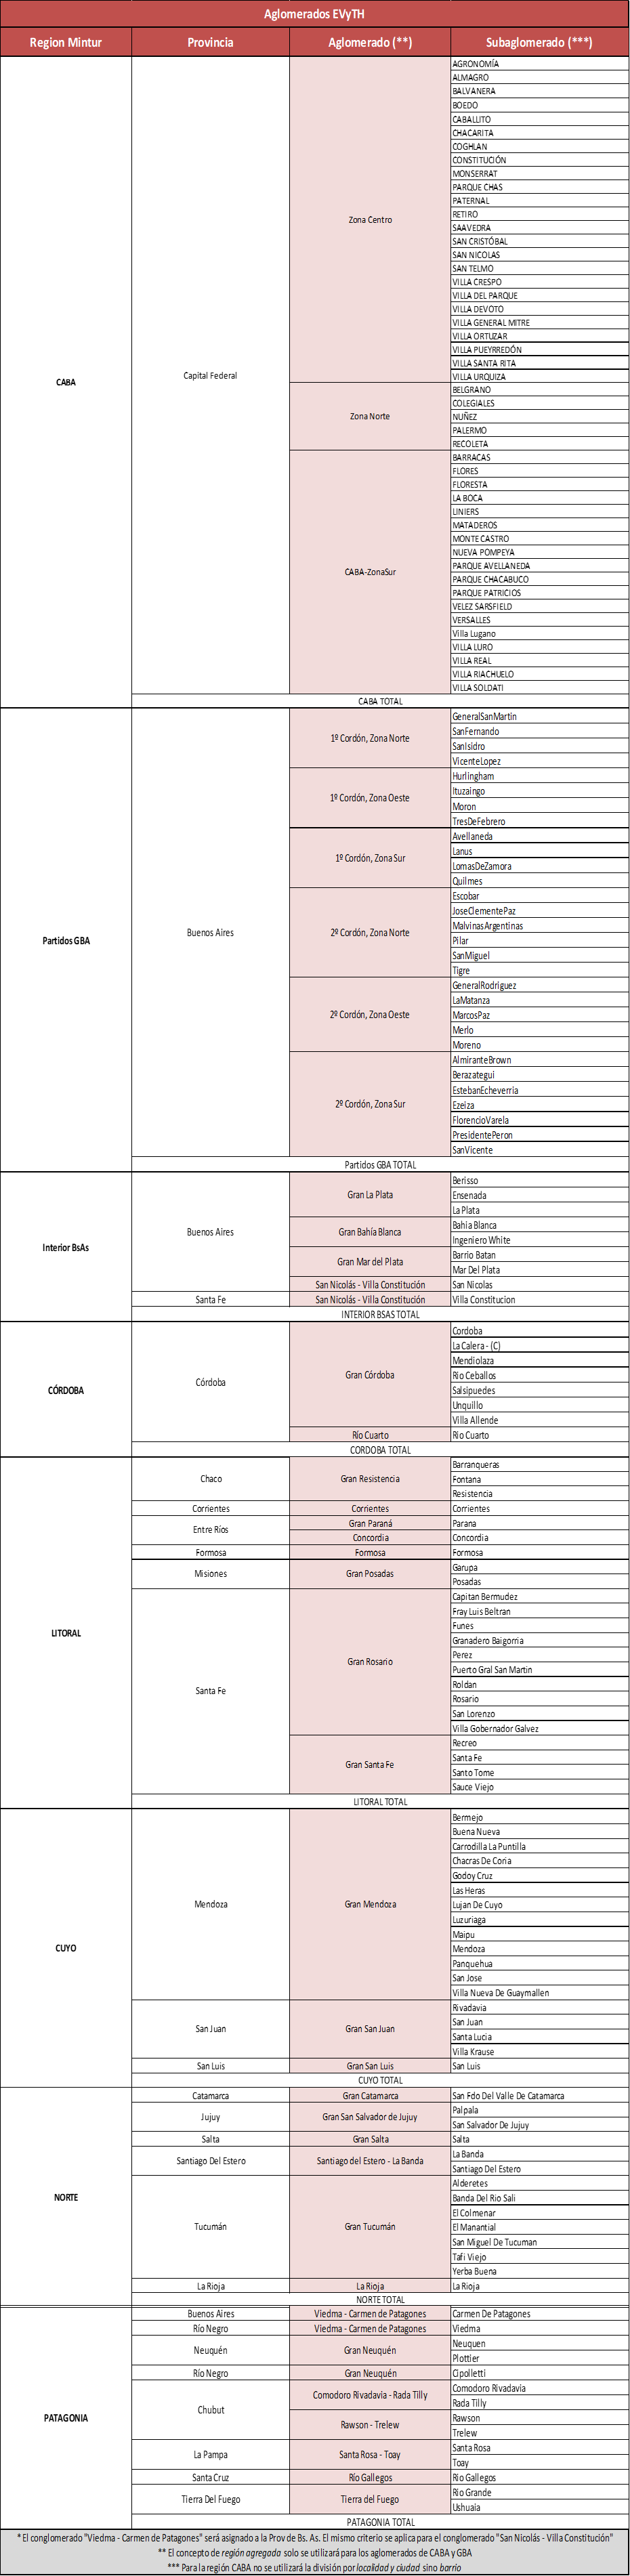
\includegraphics{cuadros_graficos/10_aglomerados.png}

En color rosa se ha marcado la zona geográfica que el Jefe de Campo seguirá para constatar que se ha relevado la cantidad de hogares necesarios para cada una estas áreas (hasta sumar tantos hogares relevados como el tamaño de la muestra exige --incorporando la metodología de reemplazo sugerida anteriormente).

\hypertarget{el-formulario-base}{%
\section{El formulario base}\label{el-formulario-base}}

Se incluye en esta sección el Formulario Base (o Cuestionario) de acuerdo a lo preestablecido en El Pliego. Previo a ello, se brinda una breve descripción de la estructura del Formulario y las principales variables relevadas.

\hypertarget{estructura-del-formulario-base}{%
\subsection{Estructura del formulario base}\label{estructura-del-formulario-base}}

Con el fin de brindar una descripción resumida del Formulario Base a aplicar durante la EVyTH-21, a continuación, se presenta su estructura y las variables relevadas.

\textbf{Cuadro 24: Estructura del Formulario Base según tipo de Pregunta para cada Viaje}

\begin{figure}

{\centering 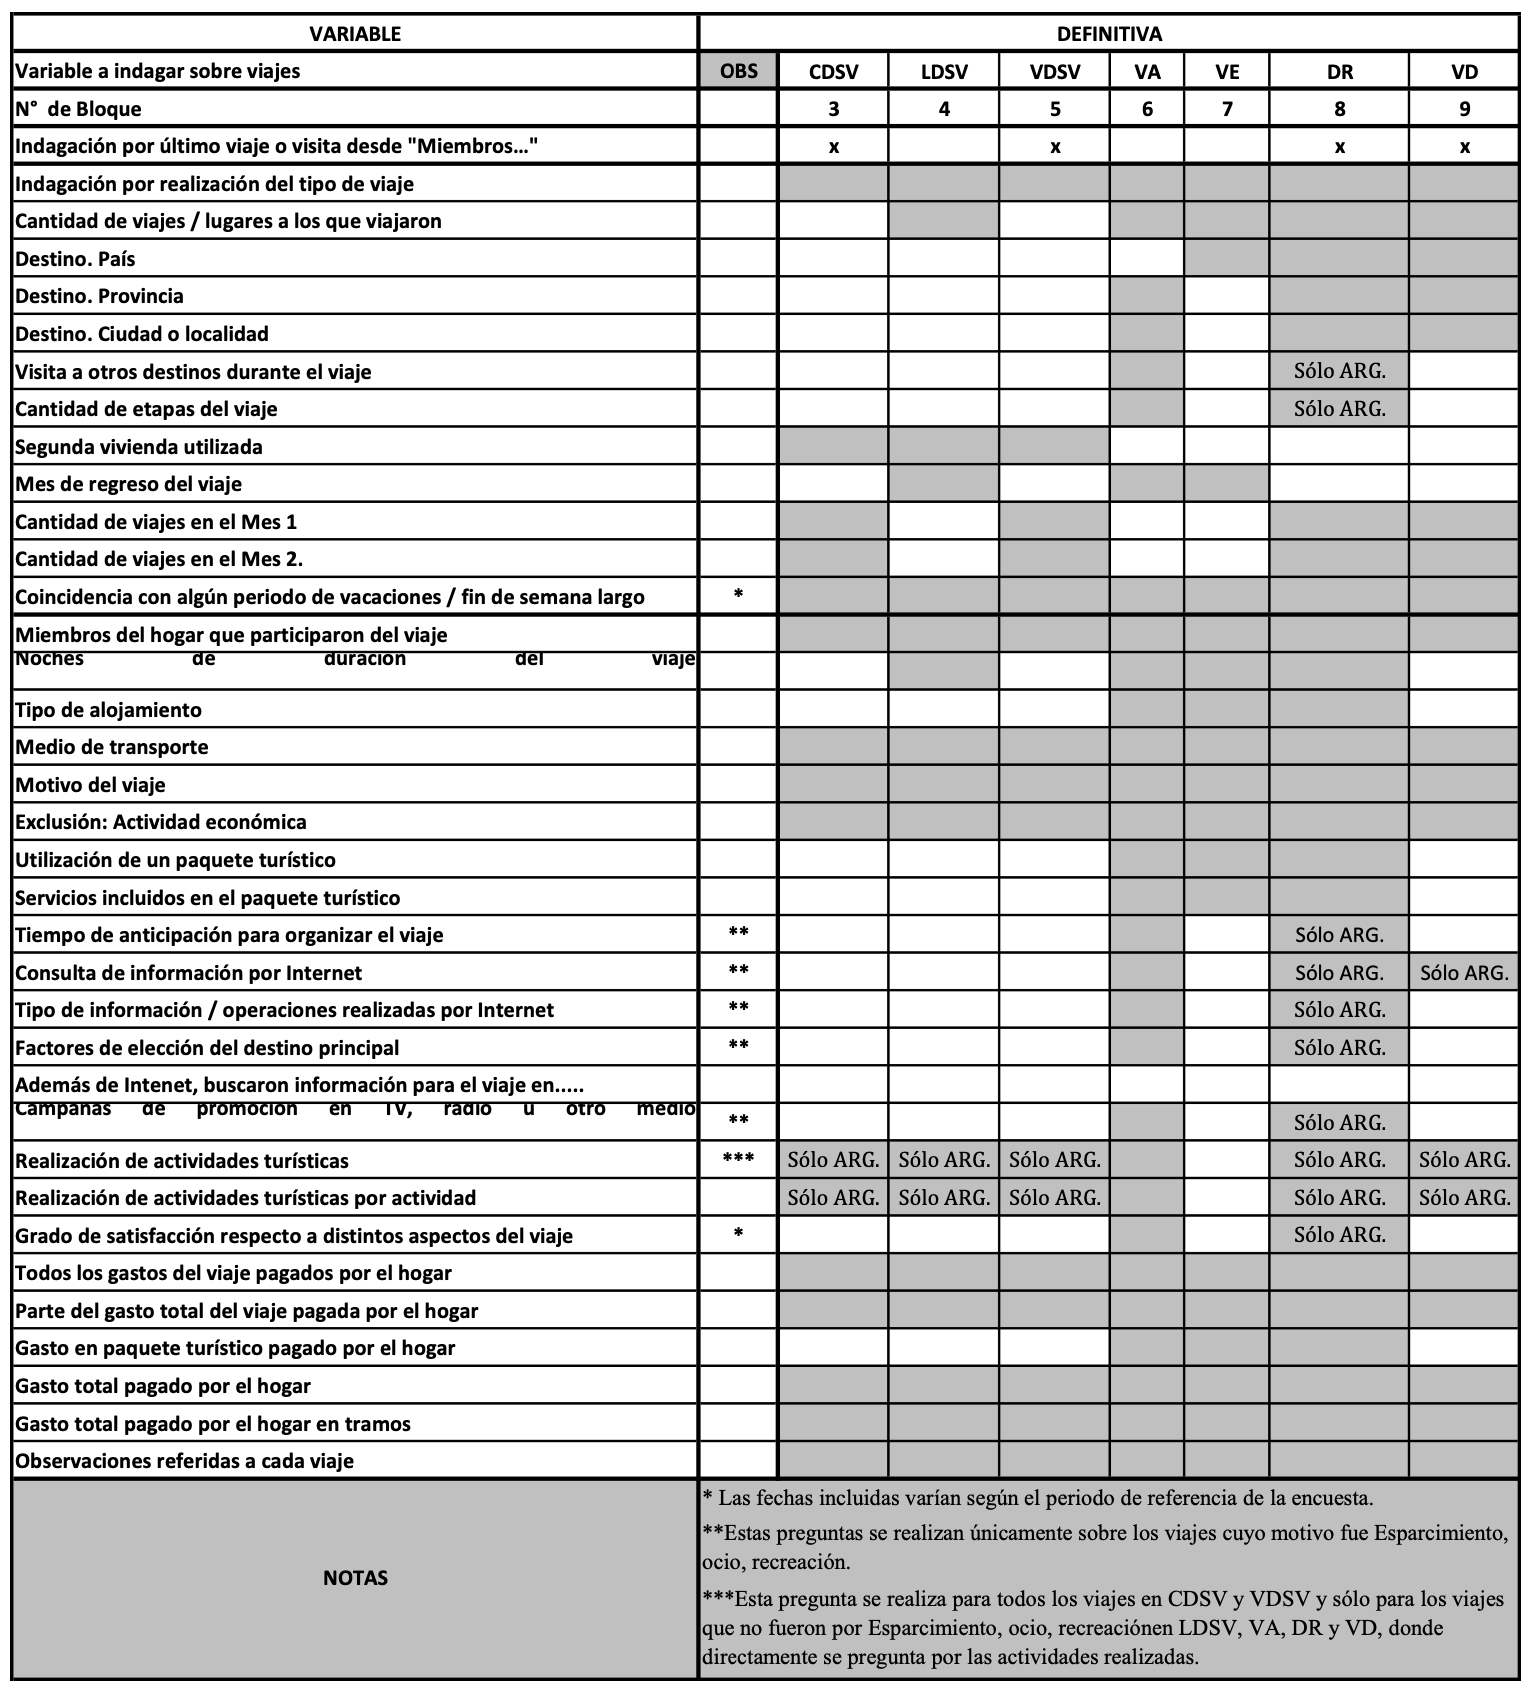
\includegraphics[width=1\linewidth]{imagenes/figura6-151} 

}

\end{figure}

Fuente: MacroConsulting

\hypertarget{cuestionario-1}{%
\subsection{Cuestionario}\label{cuestionario-1}}

Se transcribe a continuación el cuestionario que fue implementado en la EVyTH-13, con las modificaciones mencionadas en la sección 2.7.1.

Año: 201X
N° de Onda:\ldots\ldots\ldots\ldots\ldots{}
Mes de relevamiento:\ldots\ldots\ldots\ldots\ldots\ldots\ldots\ldots\ldots.
Mes 1 del periodo de referencia:\ldots\ldots\ldots\ldots\ldots\ldots\ldots\ldots\ldots.
Mes 2 del periodo de referencia:\ldots\ldots\ldots\ldots\ldots\ldots\ldots\ldots\ldots.
Región ORGANISMO CONTRATANTE:\ldots\ldots\ldots\ldots\ldots\ldots\ldots\ldots\ldots\ldots\ldots.
Provincia:\ldots\ldots\ldots\ldots\ldots\ldots\ldots\ldots\ldots\ldots\ldots\ldots\ldots\ldots..
Ciudad:\ldots\ldots\ldots\ldots\ldots\ldots\ldots\ldots\ldots\ldots\ldots\ldots\ldots\ldots\ldots\ldots{}
N° de teléfono:\ldots\ldots\ldots\ldots\ldots\ldots\ldots\ldots\ldots\ldots\ldots\ldots{}
Envío de carta: Si No
Número de llamado: 1° 2° 3°

\textbf{PRESENTACIÓN}
Hola, mi nombre es \ldots\ldots.. y hablo de parte del Ministerio de Turismo de la Nación, estamos haciendo la encuesta sobre viajes. ¿Podría hacerle algunas preguntas? Información adicional:
Su hogar fue seleccionado al azar para responder una encuesta sobre si realizaron o no viajes y, en caso de haber hecho viajes, sobre sus características.
Su colaboración es muy importante y la información que nos brinde está protegida por la Ley Nacional de Secreto Estadístico. Sus datos son anónimos y confidenciales y sólo serán utilizados con fines estadísticos.

\begin{figure}

{\centering 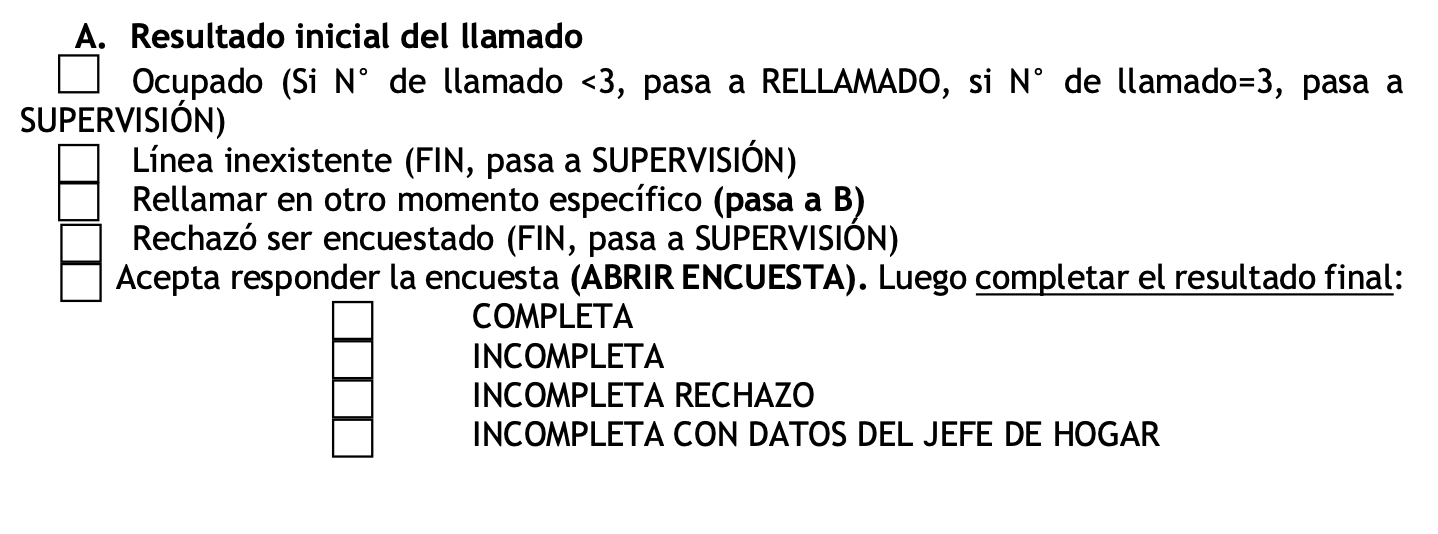
\includegraphics[width=1\linewidth]{imagenes/figura6-152} 

}

\end{figure}
\begin{figure}

{\centering 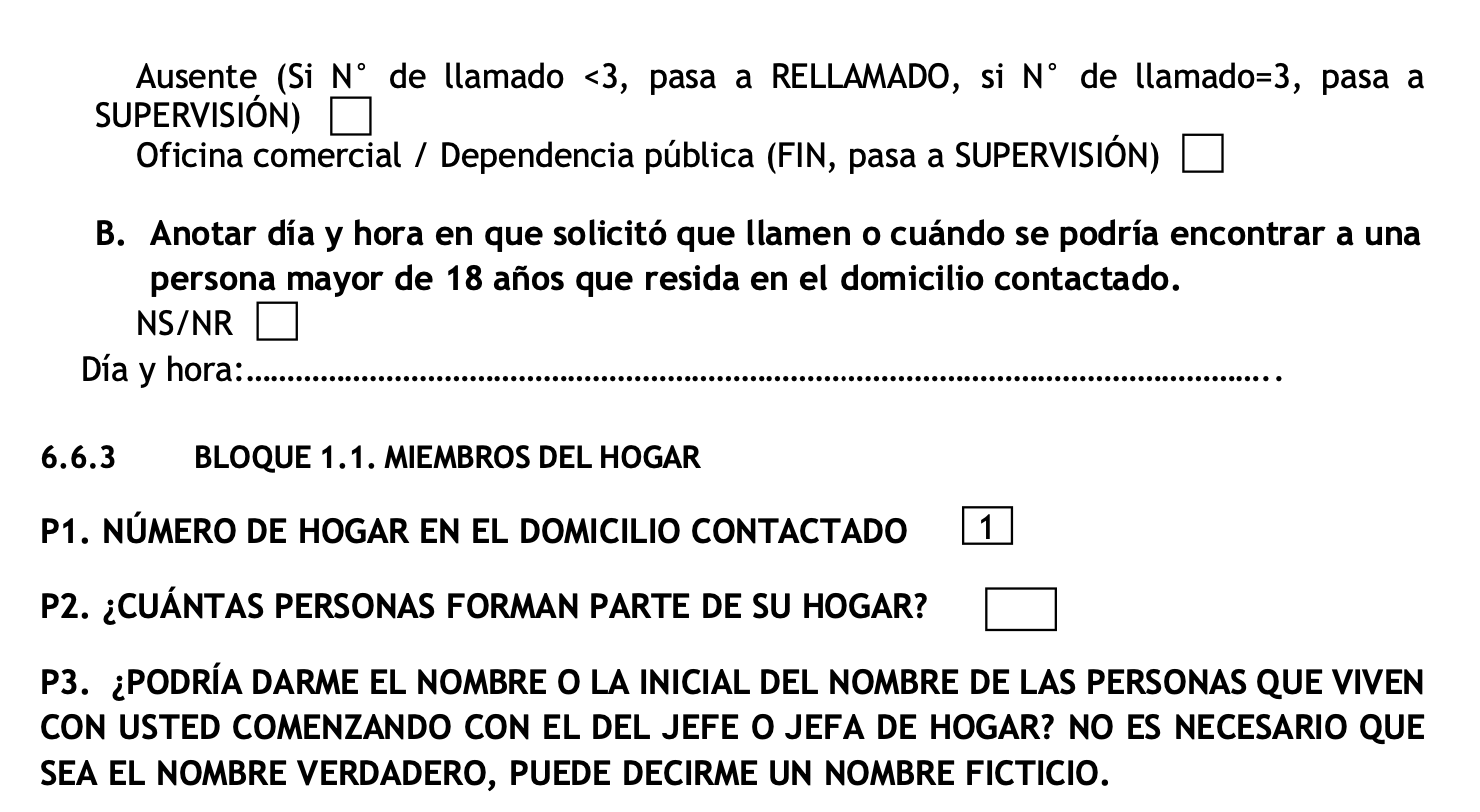
\includegraphics[width=1\linewidth]{imagenes/figura6-153} 

}

\end{figure}
\begin{figure}

{\centering 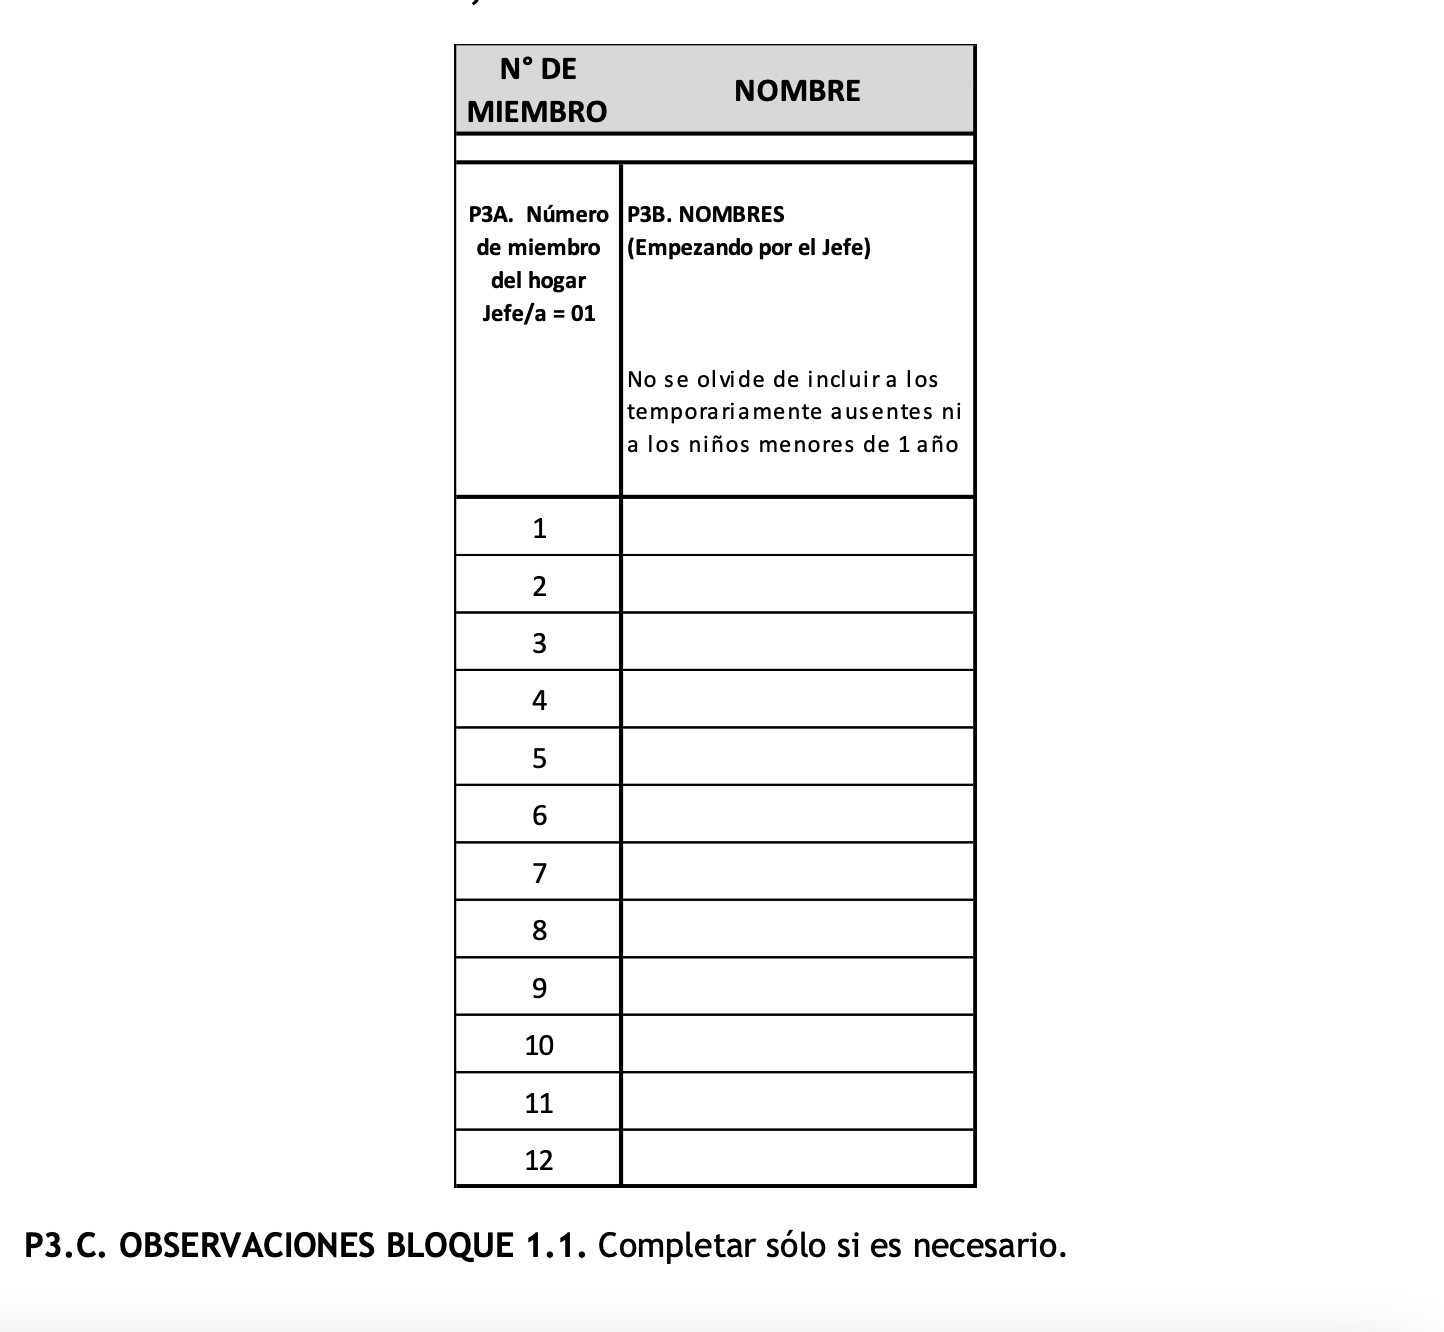
\includegraphics[width=1\linewidth]{imagenes/figura6-154} 

}

\end{figure}

\hypertarget{bloque-2.-segunda-vivienda}{%
\subsection{Bloque 2. Segunda vivienda}\label{bloque-2.-segunda-vivienda}}

\begin{figure}

{\centering 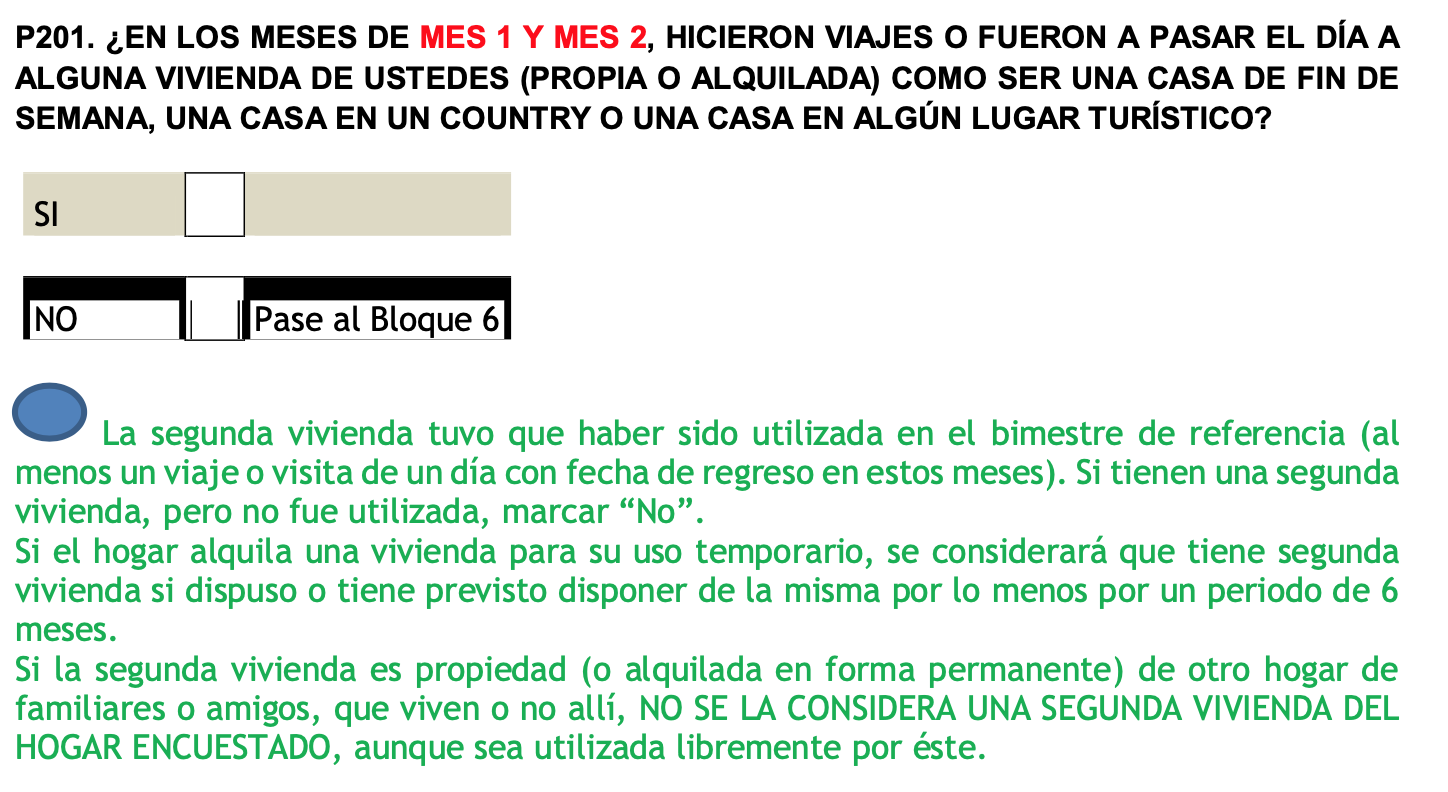
\includegraphics[width=1\linewidth]{imagenes/figura6-155} 

}

\end{figure}
\begin{figure}

{\centering 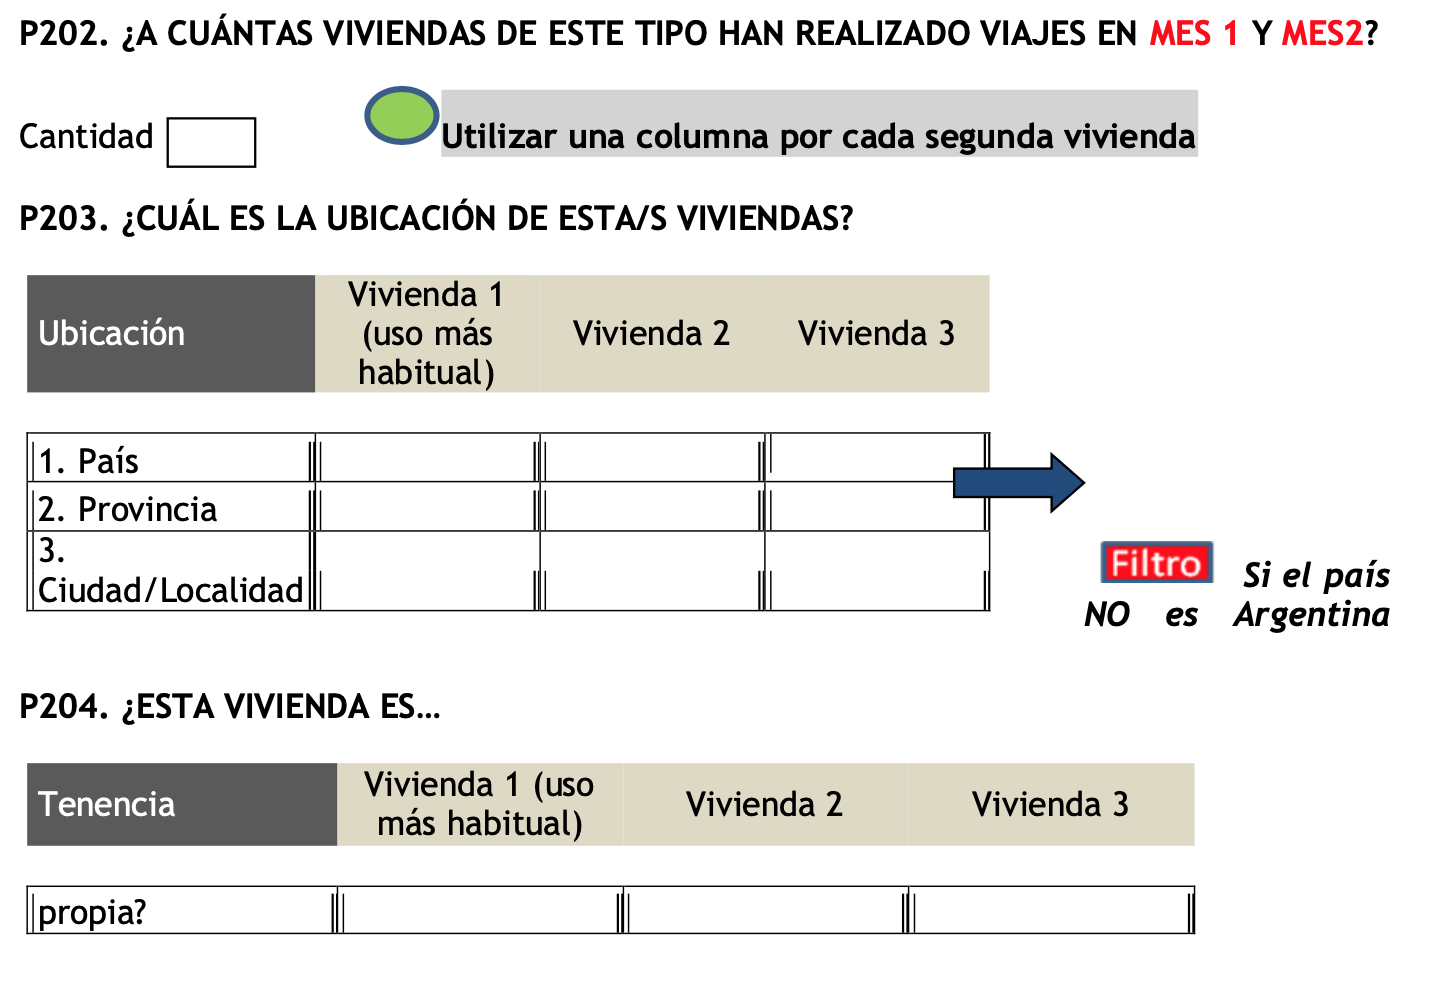
\includegraphics[width=1\linewidth]{imagenes/figura6-156} 

}

\end{figure}
\begin{figure}

{\centering 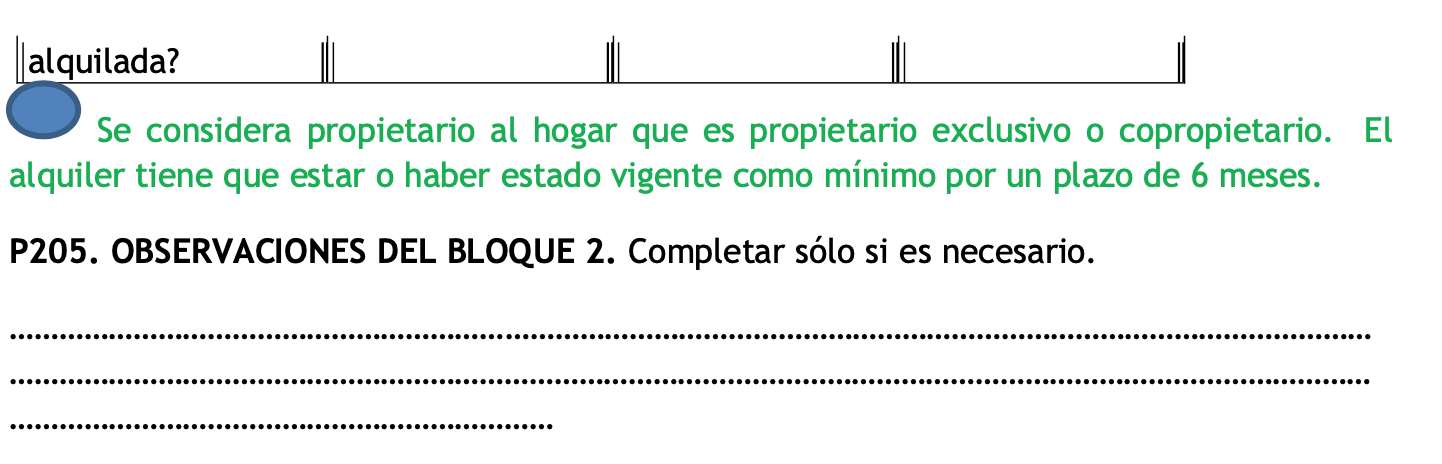
\includegraphics[width=1\linewidth]{imagenes/figura6-157} 

}

\end{figure}

\hypertarget{bloque-3.-viajes-de-corta-duraciuxf3n-a-segundas-viviendas}{%
\subsection{Bloque 3. Viajes de corta duración a segundas viviendas}\label{bloque-3.-viajes-de-corta-duraciuxf3n-a-segundas-viviendas}}

``AHORA LE VOY A PREGUNTAR POR LOS VIAJES A ESAS VIVIENDAS''

\textbf{P301.} ¿EN LOS MESES DE \textbf{MES 1 y MES 2}, UD. O ALGÚN INTEGRANTE DEL HOGAR HICIERON VIAJES A ALGUNAS DE ESTA/S VIVIENDA/S, PASANDO ALLÍ 1, 2 O 3 NOCHES?

\begin{figure}

{\centering 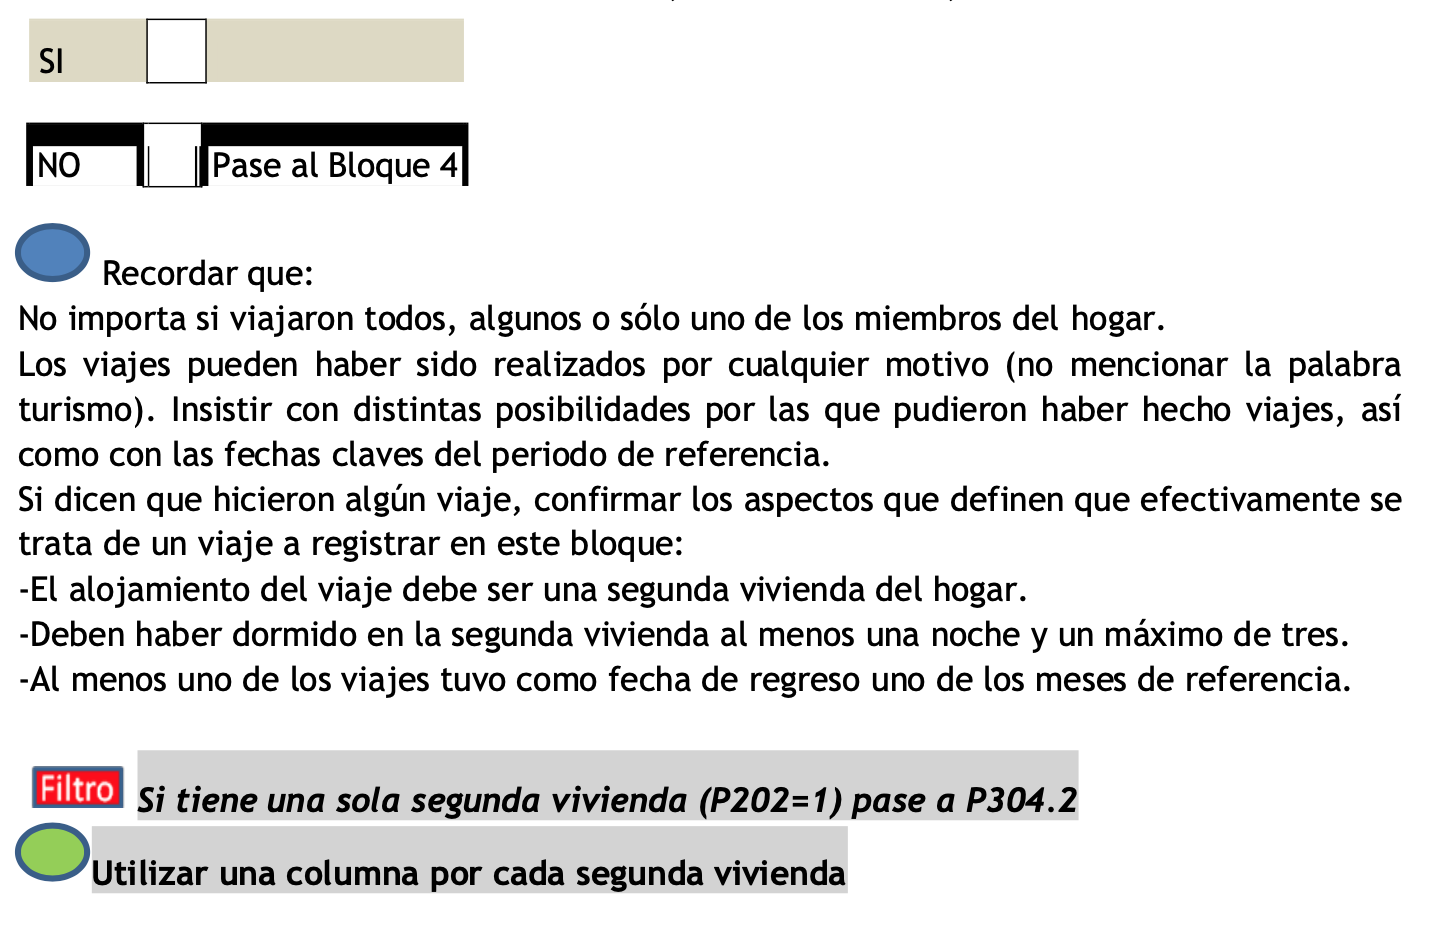
\includegraphics[width=1\linewidth]{imagenes/figura6-158} 

}

\end{figure}

\textbf{P303.2} ¿REALIZARON VIAJES DE 1 A 3 NOCHES DE DURACIÓN A LA VIVIENDA UBICADA EN
\textbf{\ldots\ldots{}}

Indague por cada segunda vivienda de la que dispone el hogar

\begin{figure}

{\centering 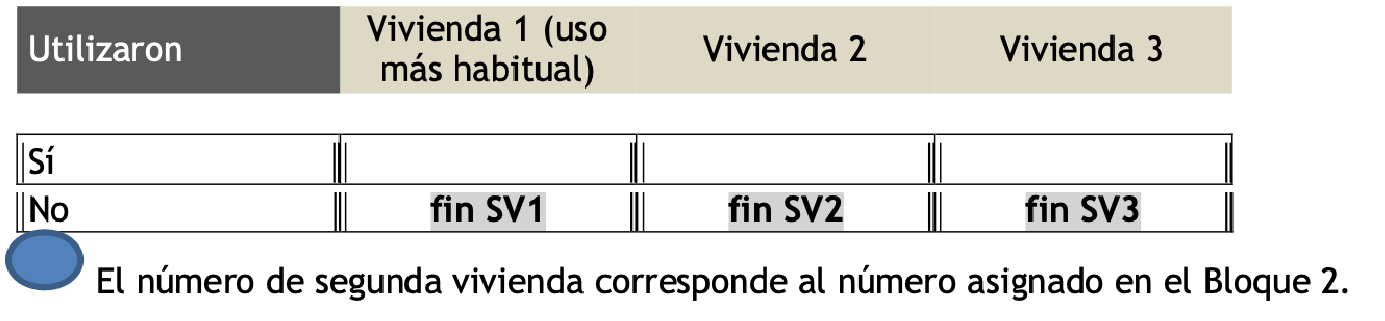
\includegraphics[width=1\linewidth]{imagenes/figura6-159} 

}

\end{figure}

\textbf{P304.2.} ¿CUÁNTOS VIAJES DE ENTRE 1 Y 3 NOCHES HICIERON EN \textbf{MES 1 Y CUÁNTOS EN MES 2?}

Anotar la cantidad. Si en uno de los meses no realizaron viajes registrar 0 (cero). Si tiene más de una segunda vivienda, preguntar cuántos por cada una.

\begin{figure}

{\centering 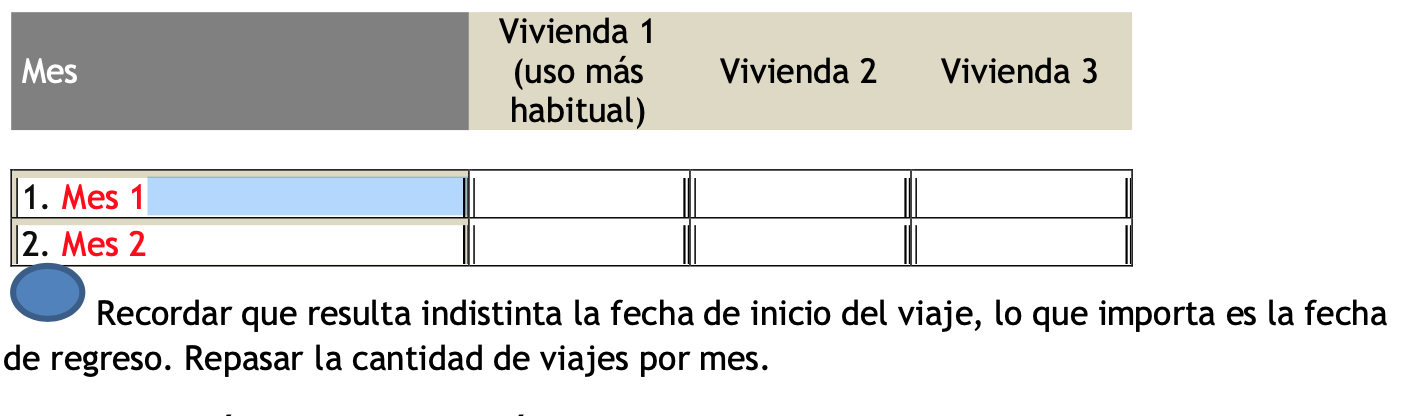
\includegraphics[width=1\linewidth]{imagenes/figura6-160} 

}

\end{figure}

\textbf{P305.2.} ¿ALGÚN VIAJE COINCIDIÓ CON \ldots.

Leer todas las opciones. Anotar en cada una alguno de los siguientes códigos: Si=1, No=2, NS/NR=9.

\begin{figure}

{\centering 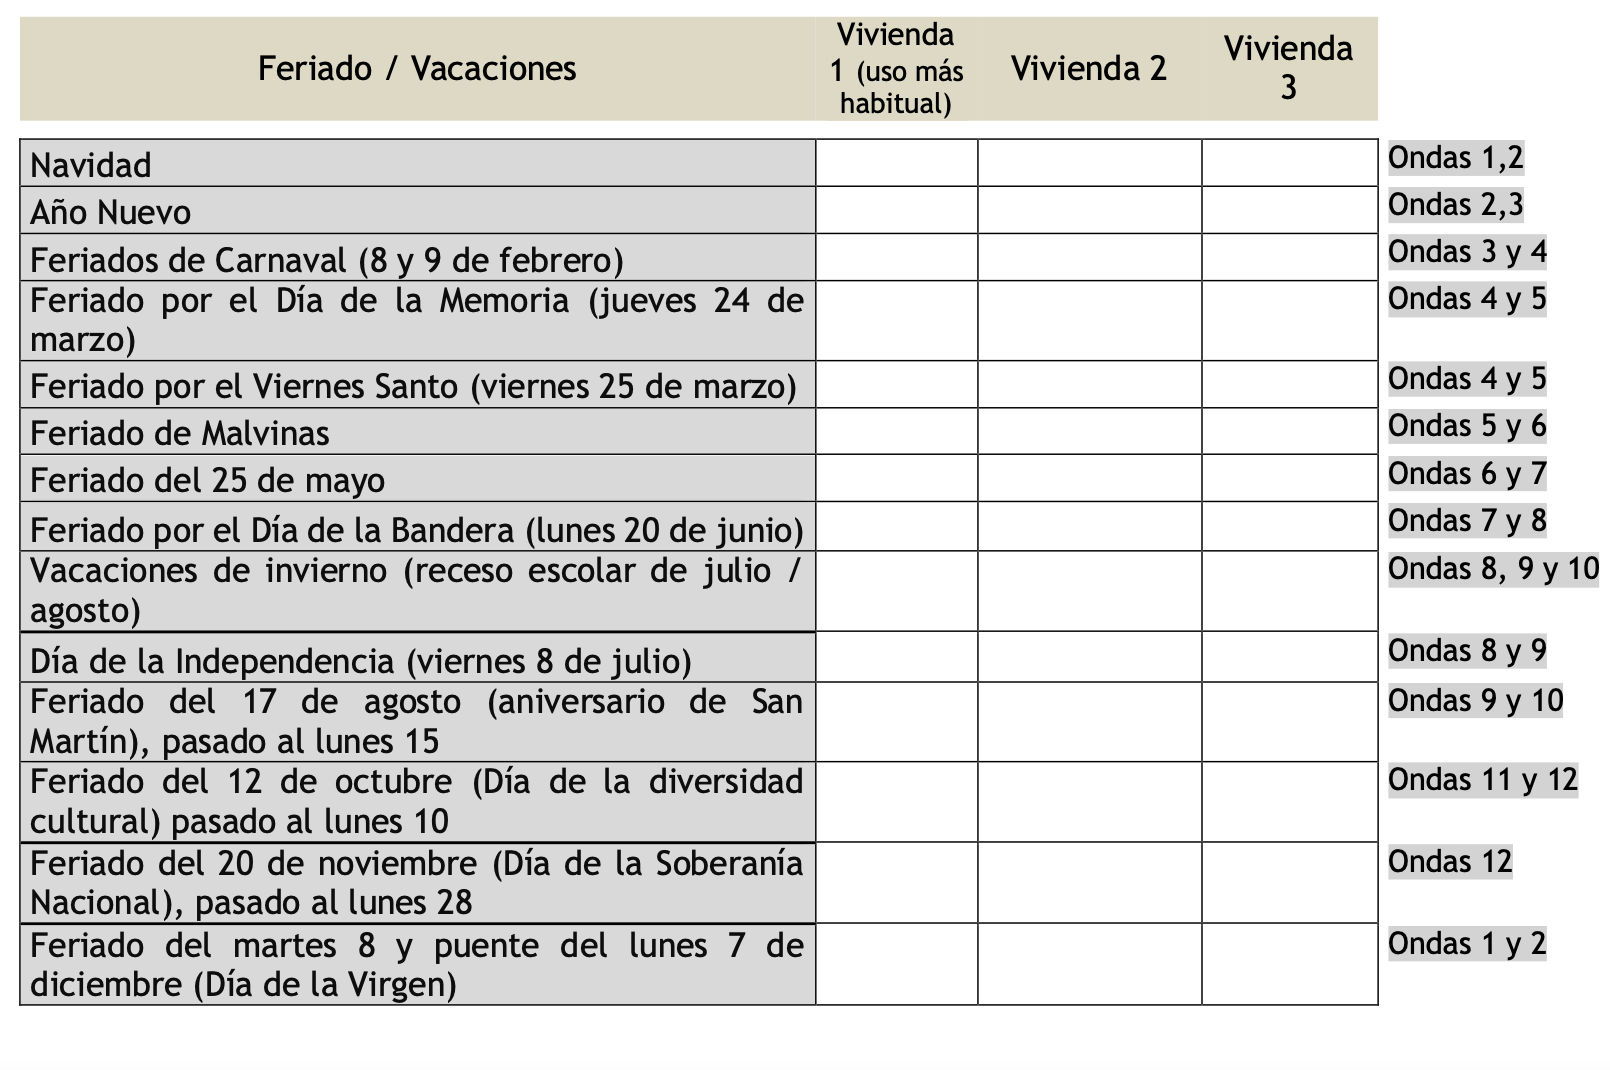
\includegraphics[width=1\linewidth]{imagenes/figura6-161} 

}

\end{figure}

\textbf{``AHORA LE VOY A HACER ALGUNAS PREGUNTAS REFERIDAS AL ÚLTIMO DE ESTOS VIAJES''}

\textbf{P306} ¿QUÉ INTEGRANTES DE SU HOGAR PARTICIPARON DEL VIAJE?
Marcar todas las opciones que correspondan. Dejar en blanco el espacio de los miembros que no viajaron.

\begin{figure}

{\centering 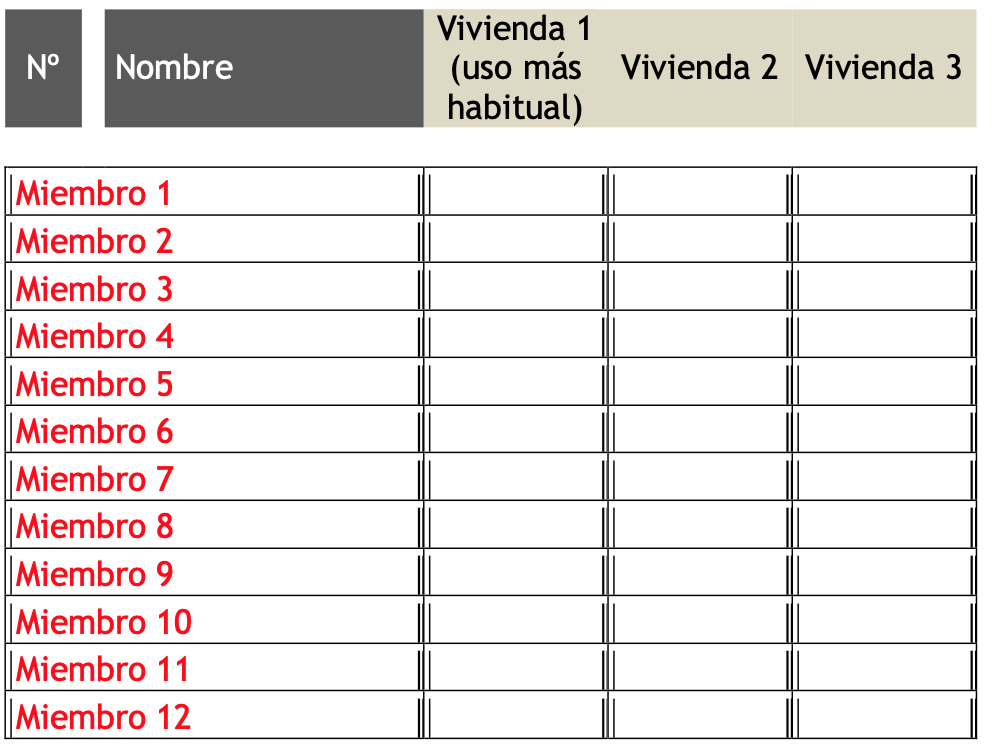
\includegraphics[width=1\linewidth]{imagenes/figura6-162} 

}

\end{figure}

\textbf{P307.2.} ¿CUÁL FUE LA DURACIÓN DEL VIAJE, DESDE QUE SALIERON HASTA QUE REGRESARON A SU HOGAR?
Anotar la cantidad de NOCHES o marcar el código de NS/NR.

\begin{figure}

{\centering 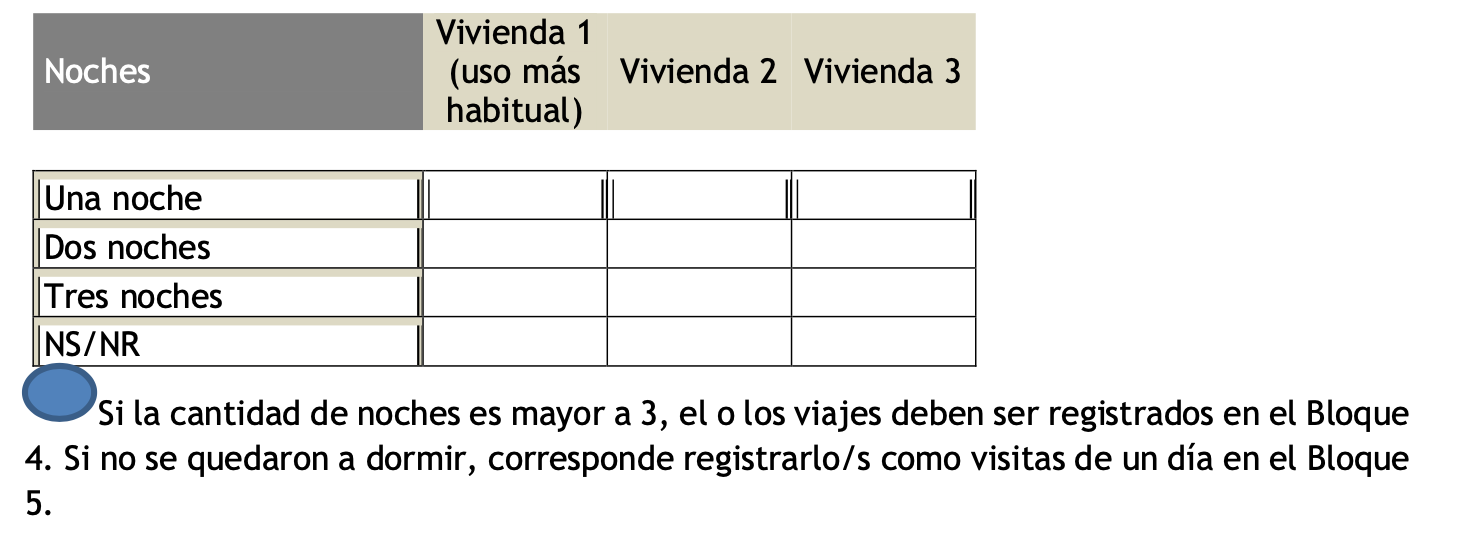
\includegraphics[width=1\linewidth]{imagenes/figura6-163} 

}

\end{figure}

\textbf{P309} ¿QUÉ MEDIO DE TRANSPORTE UTILIZARON PARA IR HASTA ALLÁ?
Marque una sola opción.

\begin{figure}

{\centering 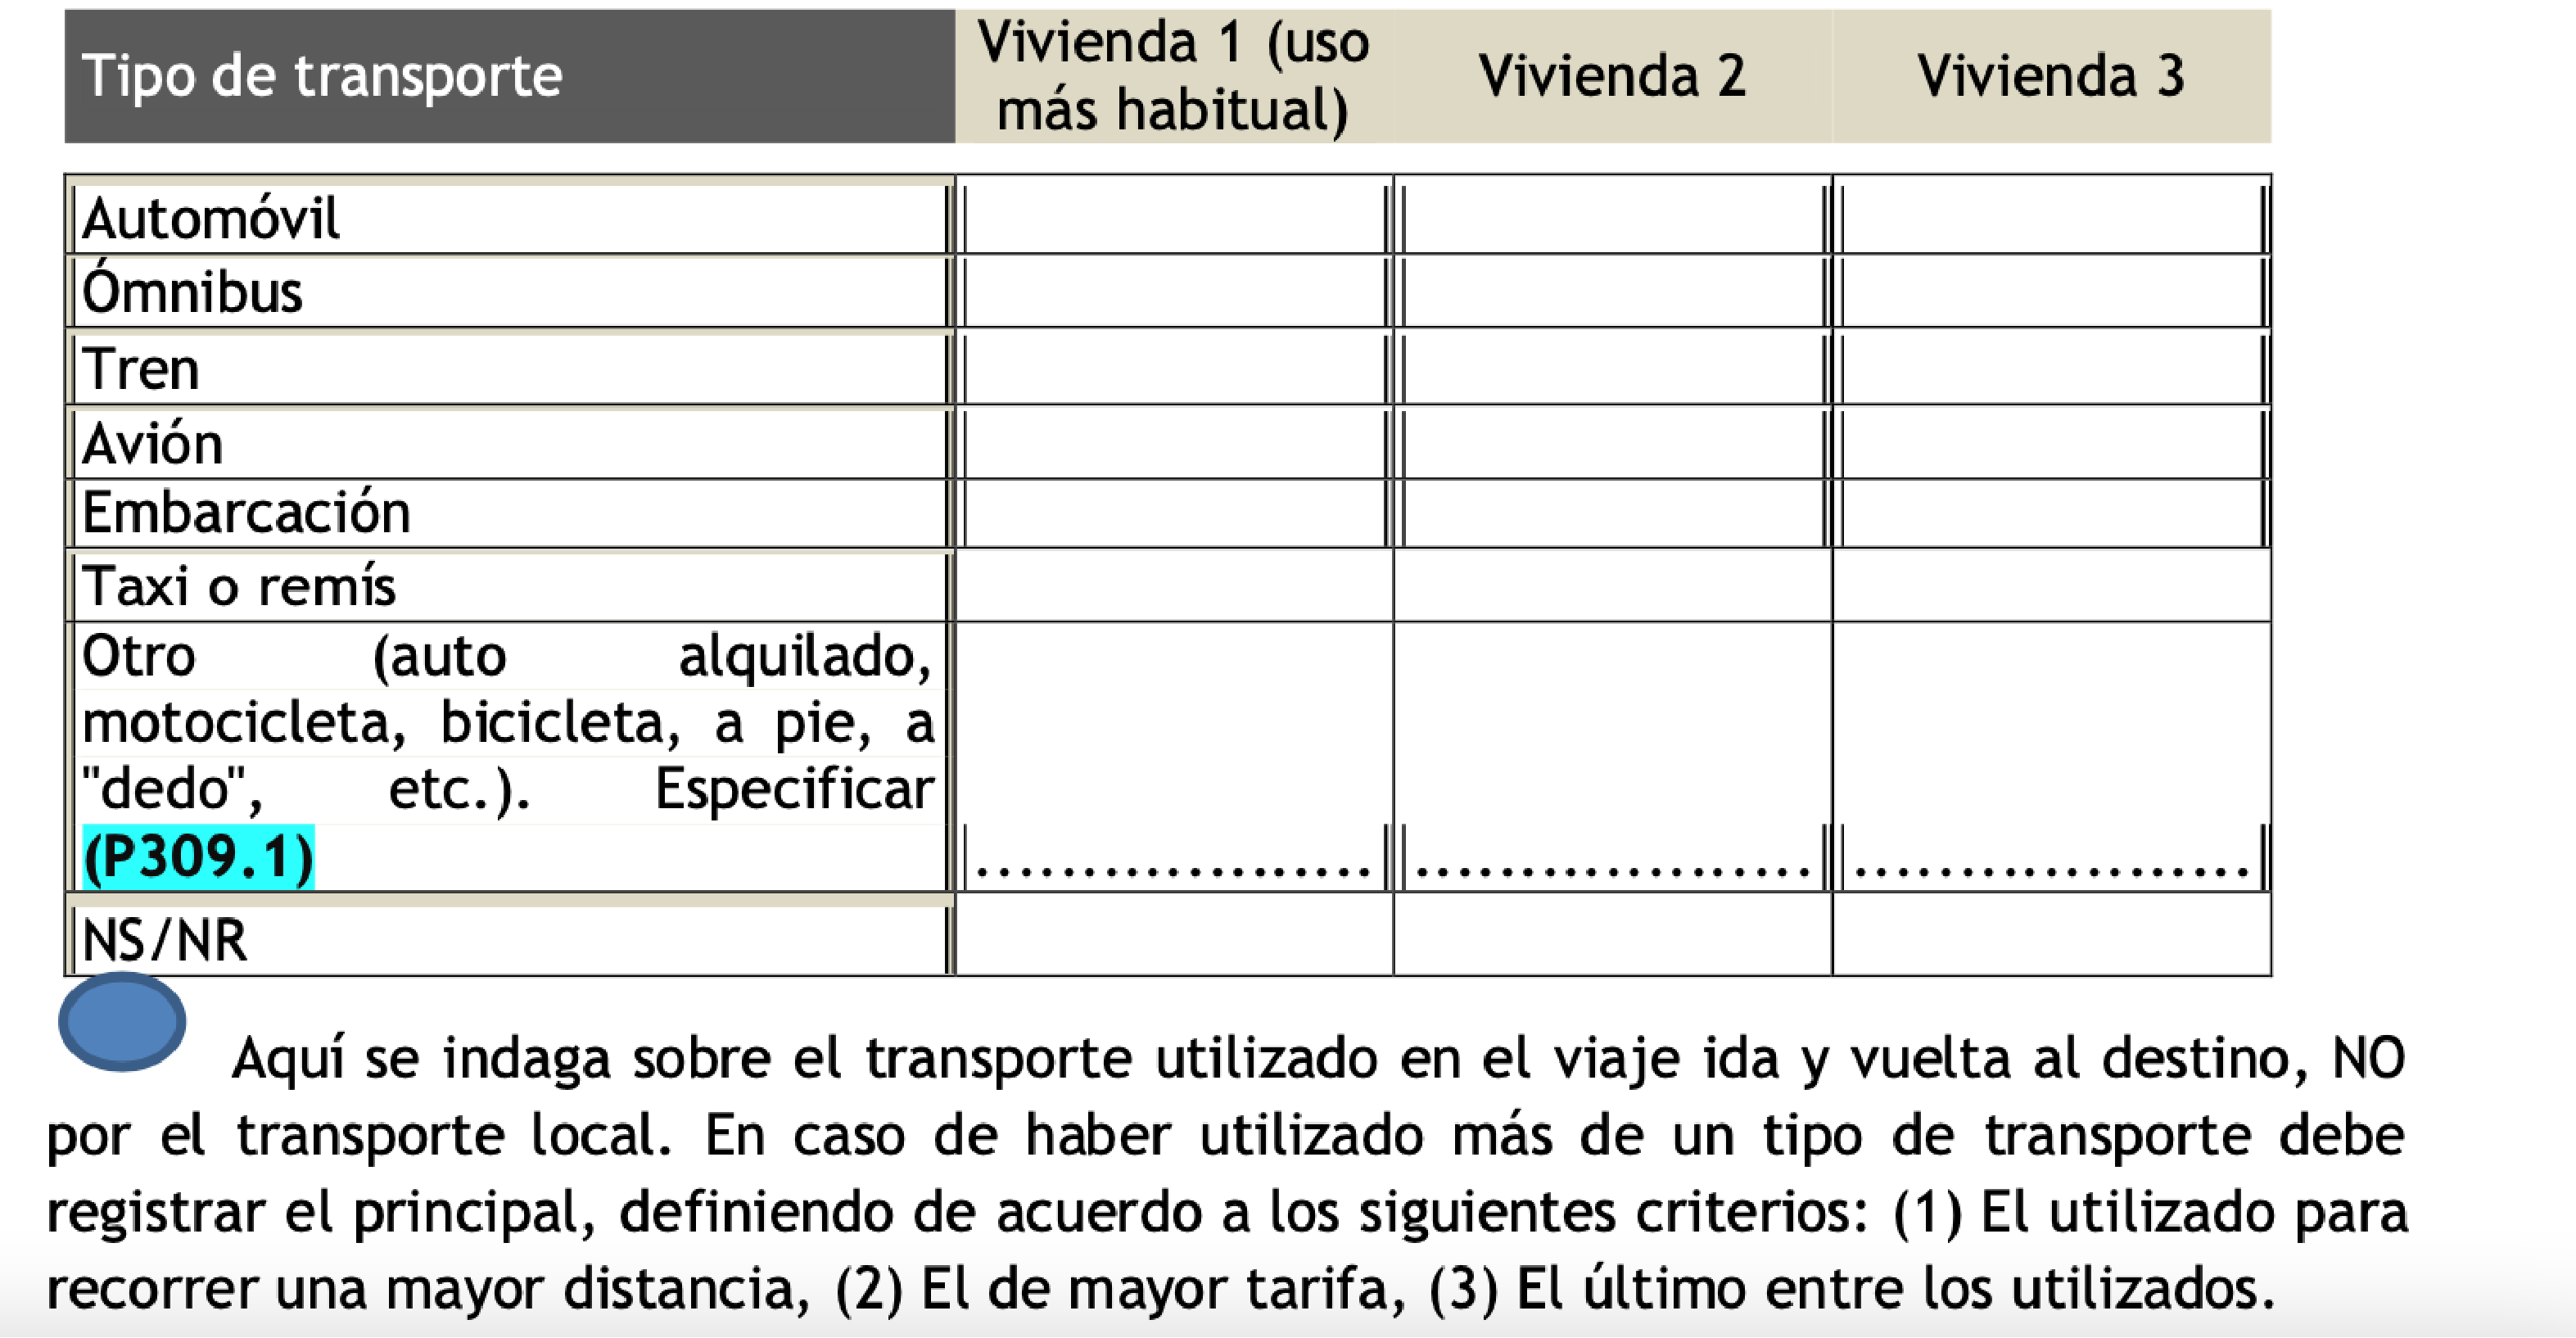
\includegraphics[width=1\linewidth]{imagenes/figura6-164} 

}

\end{figure}

\textbf{P310.1} ¿CUÁL FUE EL MOTIVO DEL VIAJE?
Marque una sola opción

\begin{figure}

{\centering 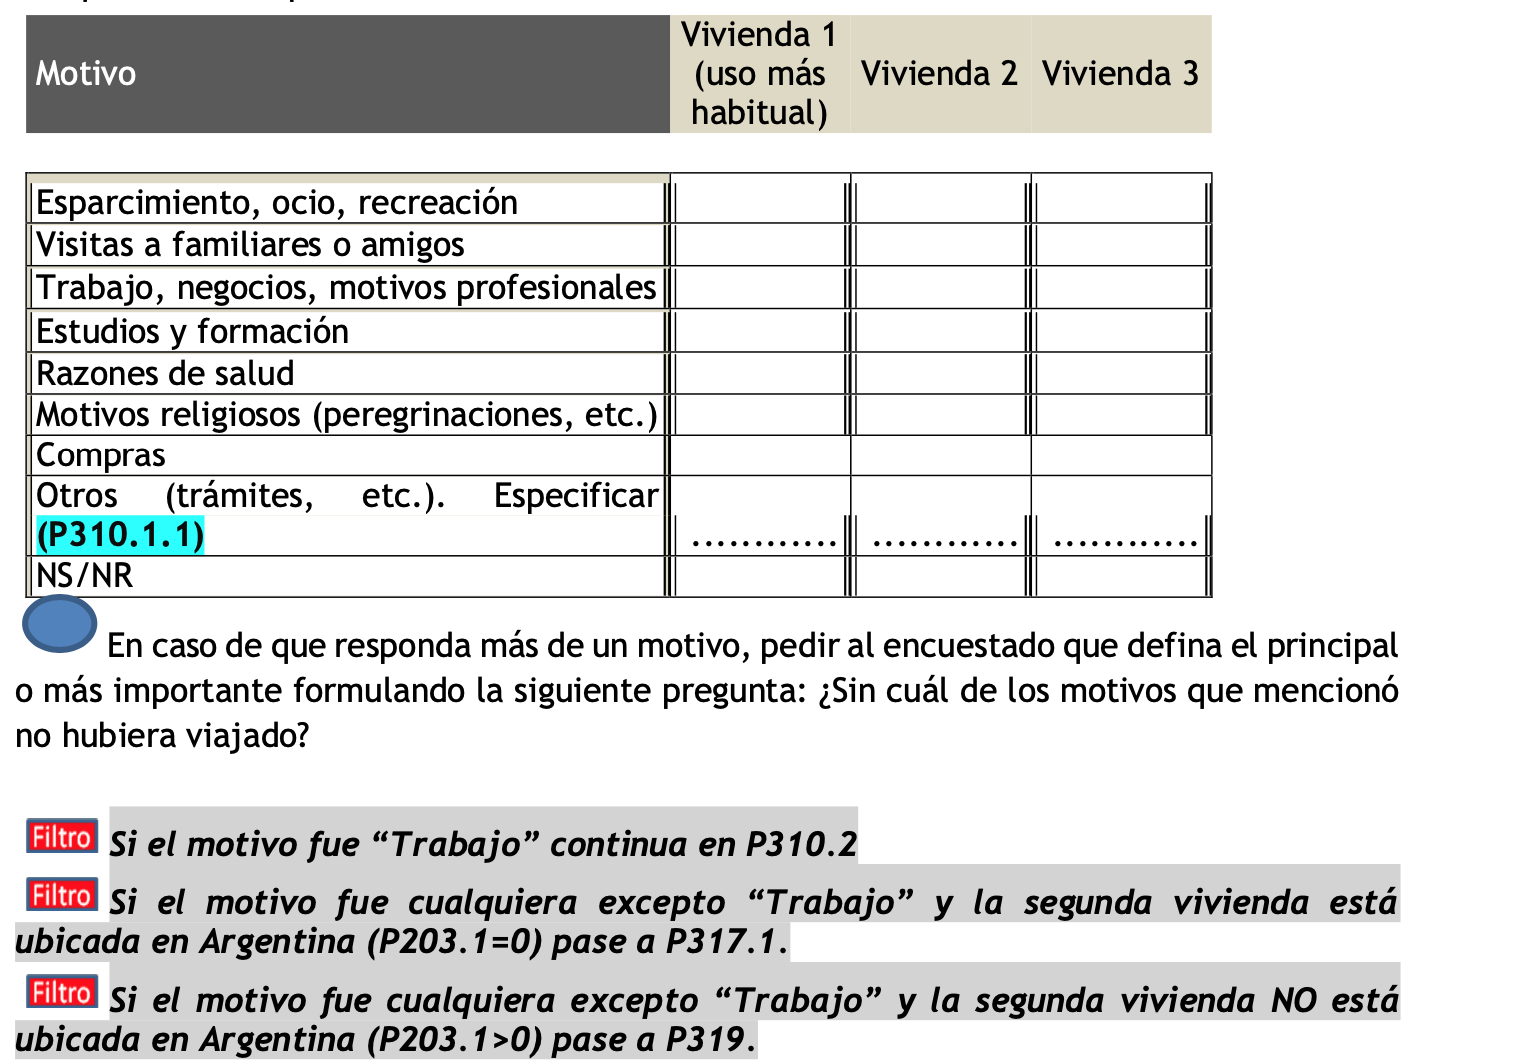
\includegraphics[width=1\linewidth]{imagenes/figura6-165} 

}

\end{figure}

\textbf{P310.2} ¿EL TRABAJO REALIZADO FUE COMO EMPLEADO DE UNA EMPRESA DEL LUGAR DE DESTINO?

¿EL DESPLAZAMIENTO O TRASLADO AL LUGAR DE DESTINO FORMÓ PARTE DE SU OFICIO (AZAFATA, VIAJANTE, CHOFER, TRANSPORTISTA, ETC.)?

Realizar la primera pregunta, si responde ``No'' formular la siguiente. Marcar ``Sí'' cuando responda afirmativamente a cualquiera de las dos preguntas.

\begin{figure}

{\centering 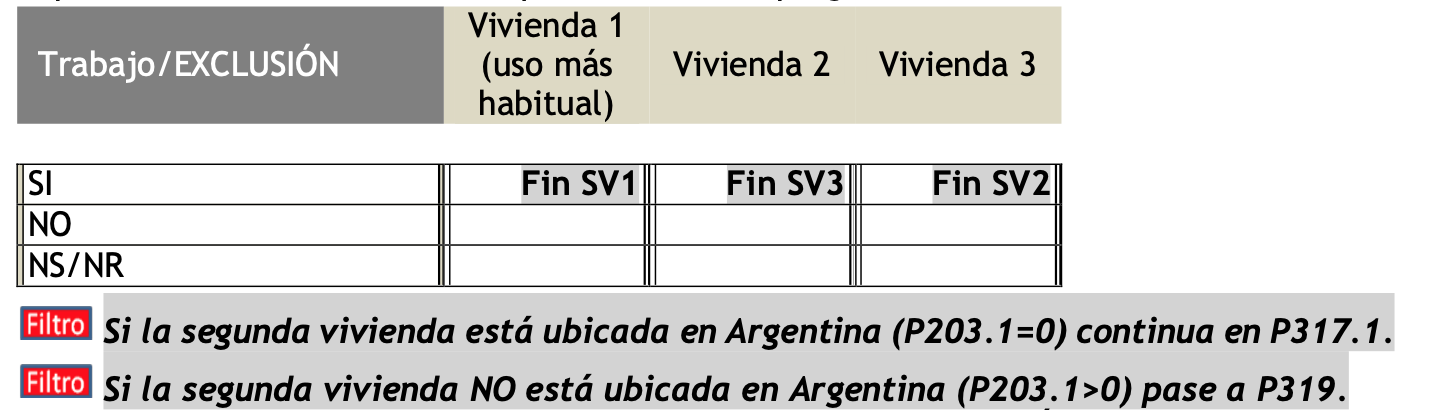
\includegraphics[width=1\linewidth]{imagenes/figura6-166} 

}

\end{figure}

\textbf{P317.1.} ¿EN ESTE VIAJE REALIZARON ALGUNA ACTIVIDAD TURÍSTICA O RECREATIVA COMO VISITAR ATRACTIVOS NATURALES O HISTÓRICOS, PRACTICAR DEPORTES NO CONVENCIONALES, IR A LA PLAYA, AL CINE, AL CASINO, U OTRAS ACTIVIDADES SIMILARES?

\begin{figure}

{\centering 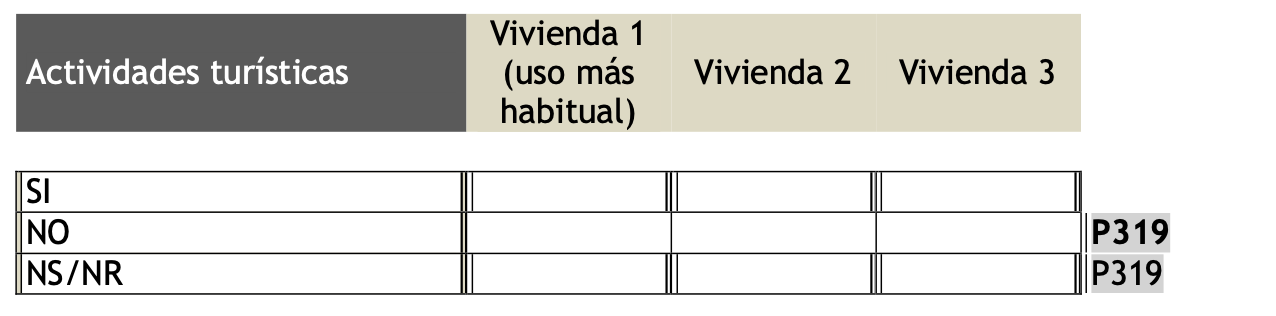
\includegraphics[width=1\linewidth]{imagenes/figura6-167} 

}

\end{figure}

\textbf{P317.2.} ¿CUÁLES DE LAS SIGUIENTES ACTIVIDADES TURÍSTICAS REALIZARON EN ESTE VIAJE? NO IMPORTA SI EN ELLAS PARTICIPARON TODOS O ALGUNO/S DE USTEDES

Leer una a una las opciones y esperar a que el entrevistado responda antes de pasar a la siguiente. Anotar en cada una alguno de los siguientes códigos: Si=1, No=2, NS/NR=9.

\begin{figure}

{\centering 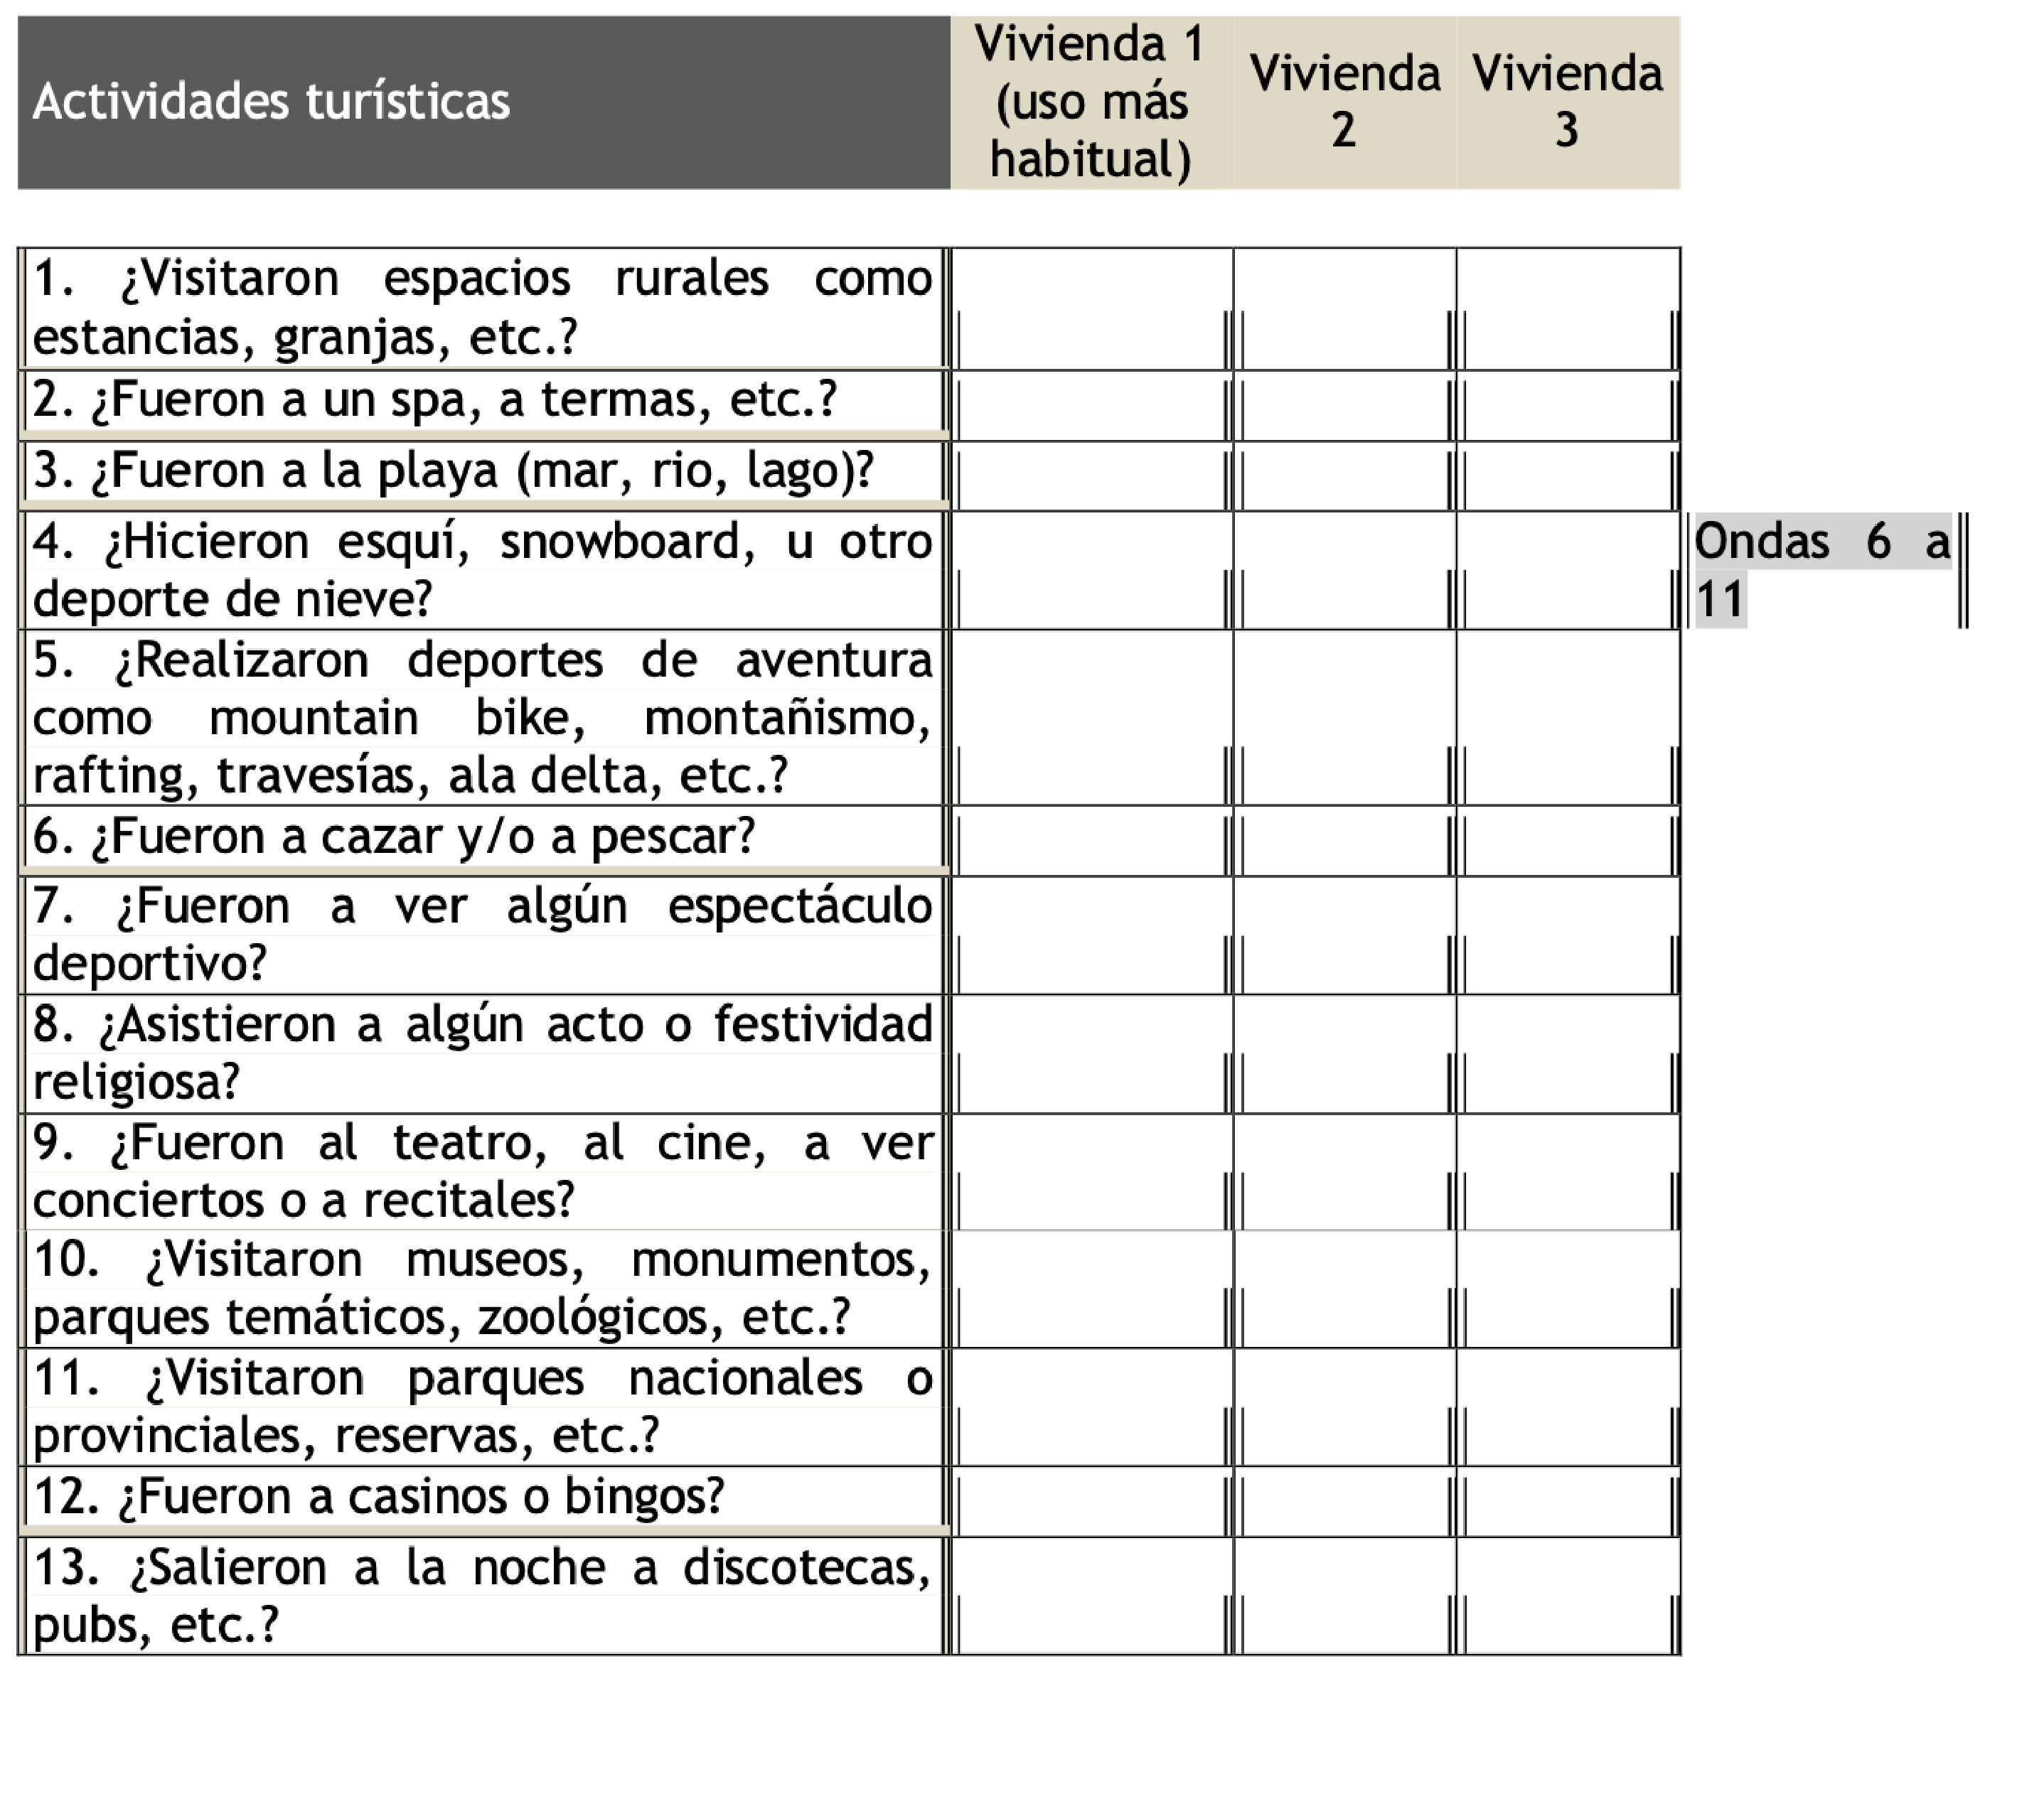
\includegraphics[width=1\linewidth]{imagenes/figura6-168} 

}

\end{figure}

\textbf{P319} ¿LOS GASTOS DEL VIAJE FUERON PAGADOS TOTALMENTE POR EL HOGAR?

\begin{figure}

{\centering 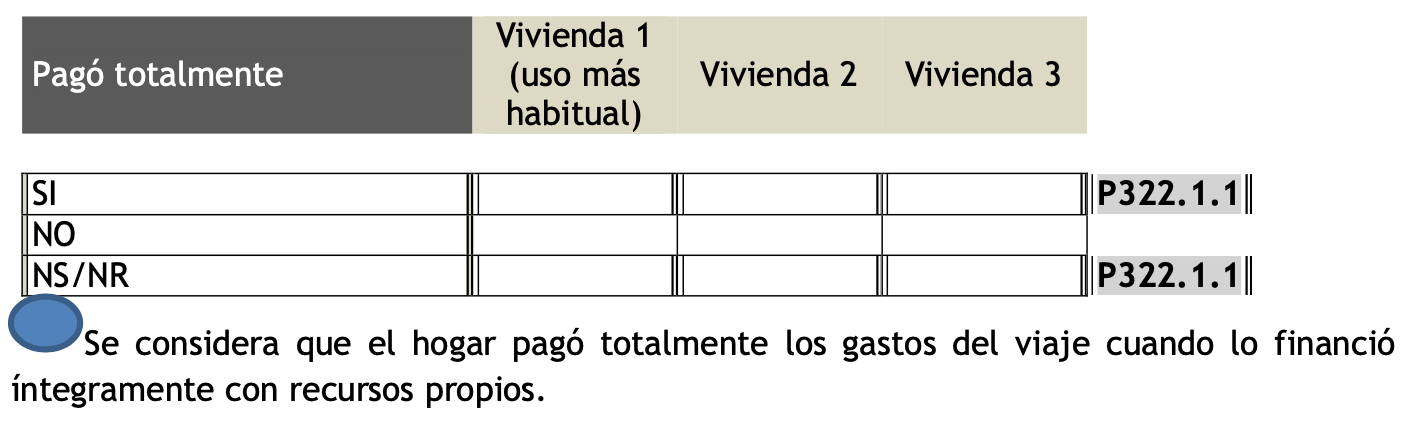
\includegraphics[width=1\linewidth]{imagenes/figura6-169} 

}

\end{figure}

\textbf{P320} ¿DE QUÉ PARTE DE LOS GASTOS SE HIZO CARGO EL HOGAR?
Marque una sola opción

\begin{figure}

{\centering 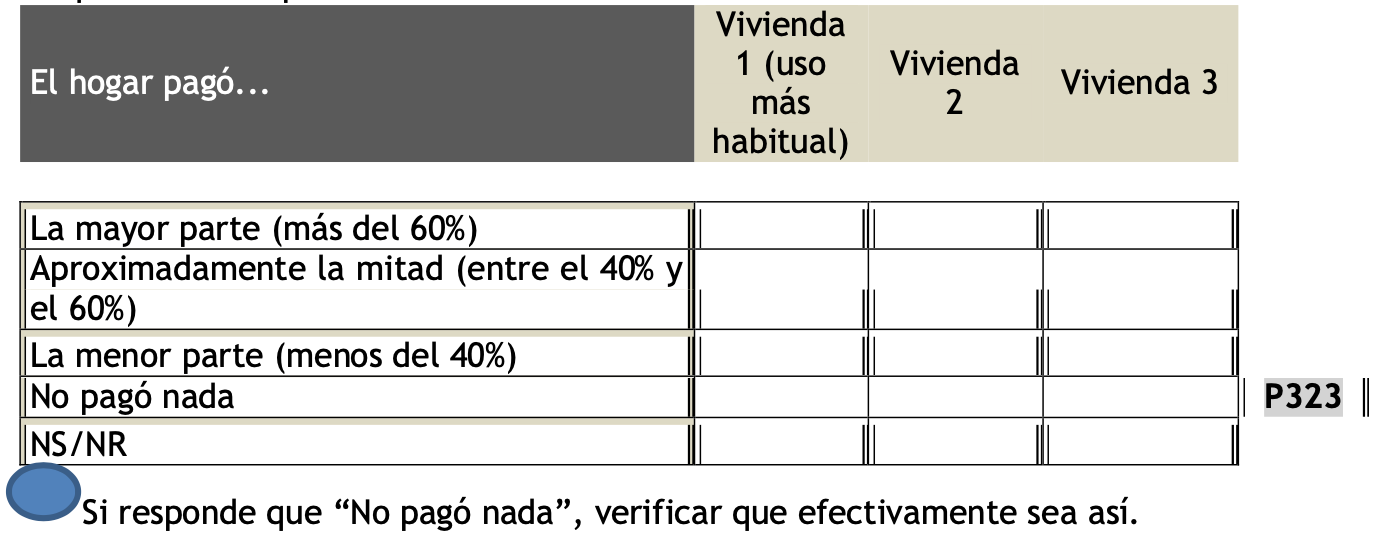
\includegraphics[width=1\linewidth]{imagenes/figura6-170} 

}

\end{figure}

\textbf{P322.1.1} APROXIMADAMENTE, ¿CUÁNTO GASTARON EN TOTAL EN EL VIAJE, INCLUYENDO
LOS GASTOS DE TODOS LOS MIEMBROS DEL HOGAR EN TRANSPORTE, COMIDAS, ETC.?

\begin{figure}

{\centering 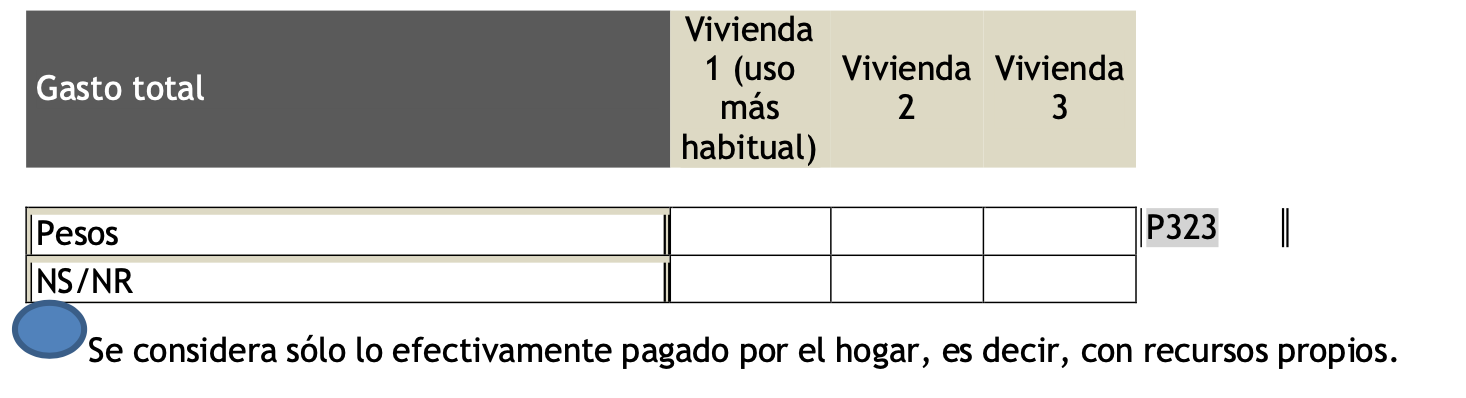
\includegraphics[width=1\linewidth]{imagenes/figura6-171} 

}

\end{figure}

\textbf{P322.1.2.3.} ¿PODRÍA DECIRME EN CUÁL DE LOS SIGUIENTES TRAMOS CREE QUE SE UBICA EL GASTO TOTAL DEL VIAJE PAGADO POR EL HOGAR?

Leer las opciones listadas y marcar la que señale el entrevistado.

\begin{figure}

{\centering 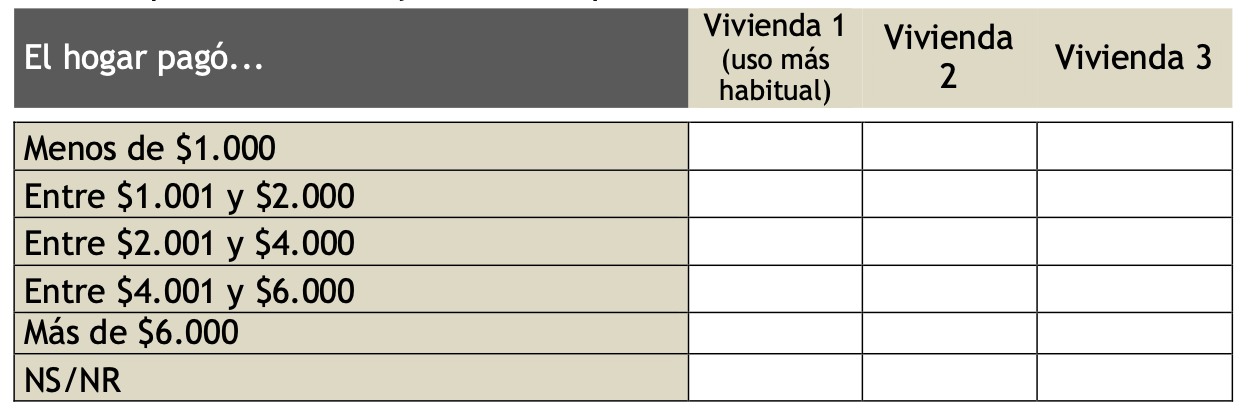
\includegraphics[width=1\linewidth]{imagenes/figura6-172} 

}

\end{figure}

\textbf{P323.} OBSERVACIONES REFERIDAS AL VIAJE
Completar sólo en caso de ser necesario.

\begin{figure}

{\centering 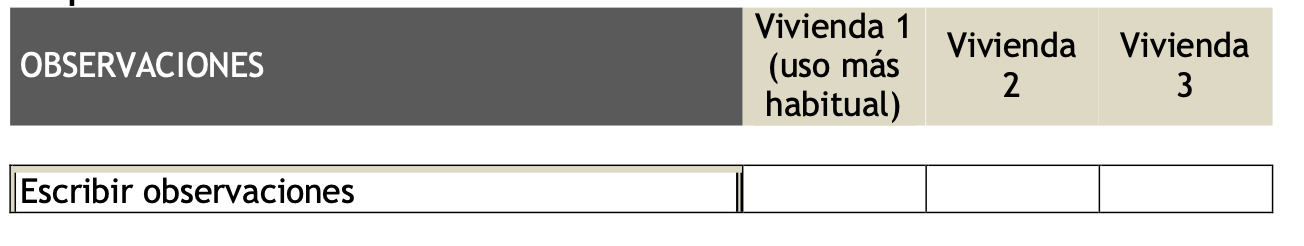
\includegraphics[width=1\linewidth]{imagenes/figura6-173} 

}

\end{figure}

\hypertarget{bloque-4.-viajes-de-larga-duraciuxf3n-a-segundas-viviendas}{%
\subsection{Bloque 4. Viajes de larga duración a segundas viviendas}\label{bloque-4.-viajes-de-larga-duraciuxf3n-a-segundas-viviendas}}

\textbf{P401.} ¿EN LOS MESES DE \textbf{MES 1 y MES 2}, UD. O ALGÚN INTEGRANTE DEL HOGAR HICIERON VIAJES A ALGUNAS DE ESTA/S VIVIENDA/S PASANDO ALLÍ 4 NOCHES O MÁS?

\begin{figure}

{\centering 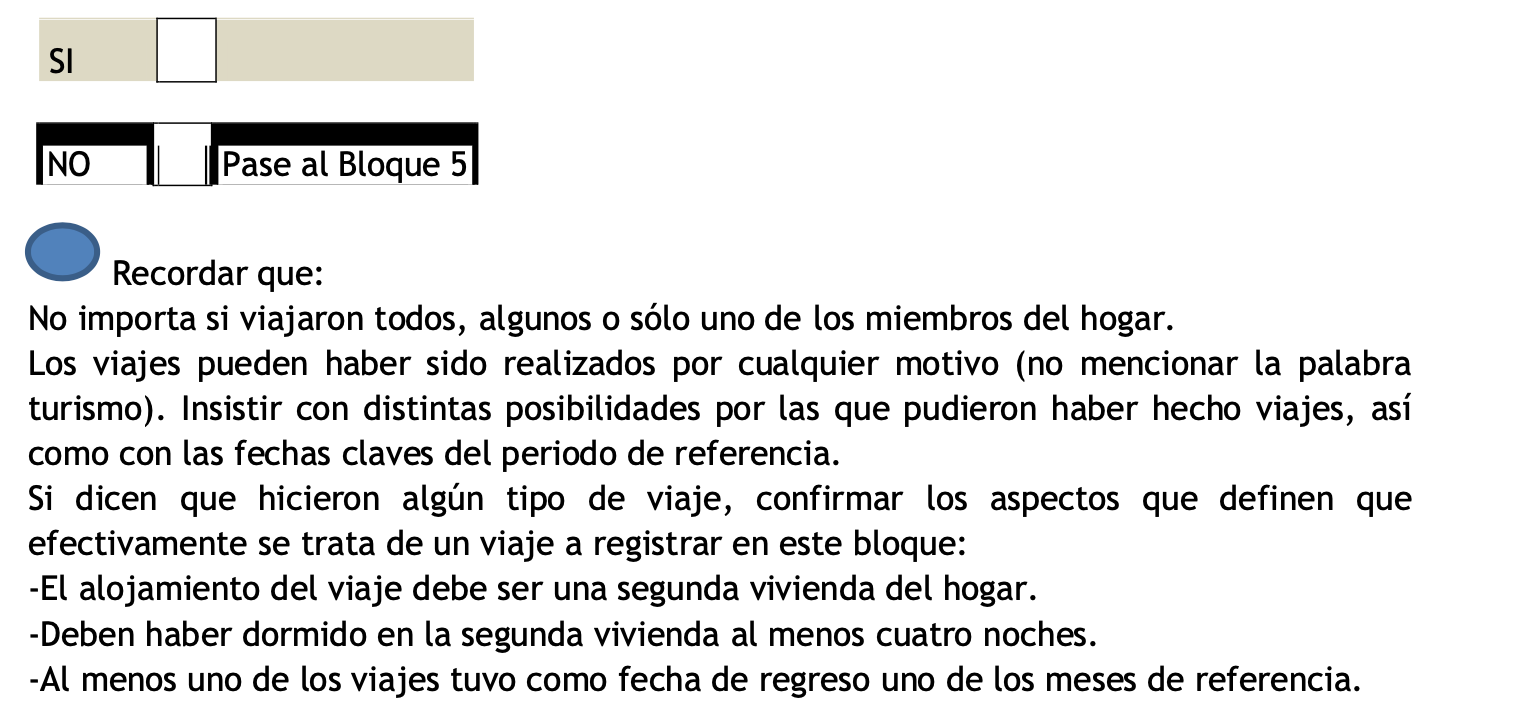
\includegraphics[width=1\linewidth]{imagenes/figura6-174} 

}

\end{figure}

\textbf{P402.} ¿CUÁNTOS VIAJES DE 4 O MÁS NOCHES HICIERON EN \textbf{MES 1 Y MES 2} A LA/S VIVIENDA/S?
Anotar la cantidad de viajes con fecha de regreso en los meses incluidos en el bimestre de referencia.

\begin{figure}

{\centering 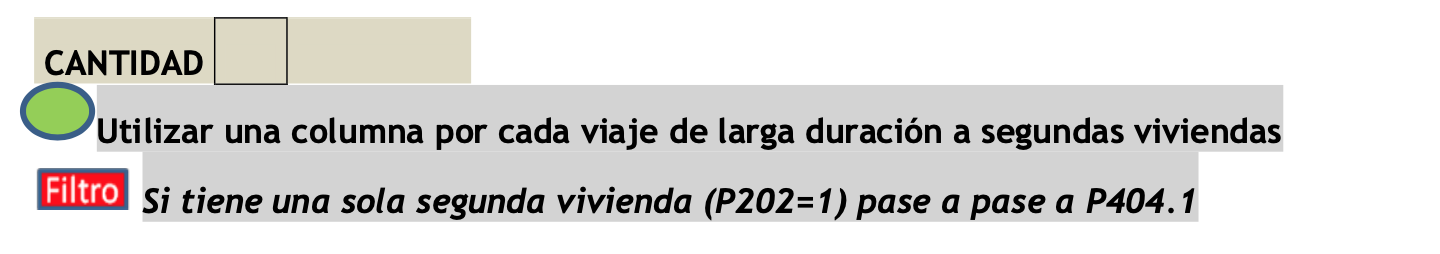
\includegraphics[width=1\linewidth]{imagenes/figura6-175} 

}

\end{figure}

\textbf{P403.3} ¿QUÉ VIVIENDA UTILIZARON EN EL VIAJE?

\begin{figure}

{\centering 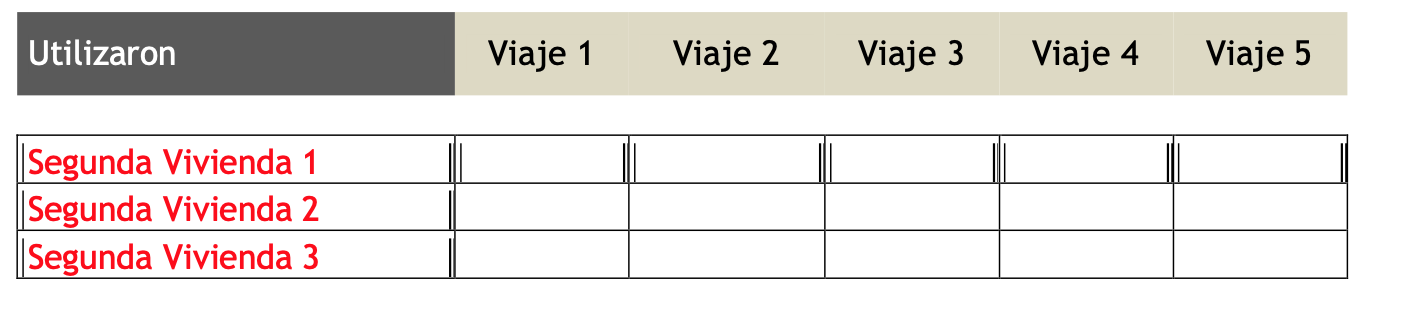
\includegraphics[width=1\linewidth]{imagenes/figura6-176} 

}

\end{figure}

\textbf{``AHORA LE VOY A HACER ALGUNAS PREGUNTAS REFERIDAS A CADA UNO DE ESTOS VIAJES. EMPECEMOS POR EL MÁS RECIENTE''}

\textbf{P404.1.} ¿EL VIAJE FUE REALIZADO EN \textbf{MES 1 O MES 2?}

\begin{figure}

{\centering 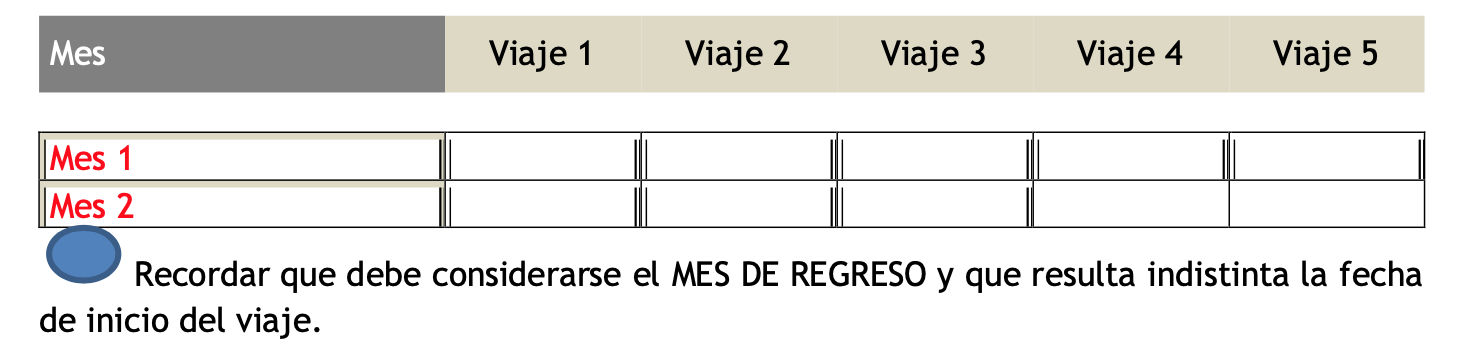
\includegraphics[width=1\linewidth]{imagenes/figura6-177} 

}

\end{figure}

\textbf{P405.2.} ¿ESTE VIAJE COINCIDIÓ CON\ldots.
Leer todas las opciones y marcar una.

\begin{figure}

{\centering 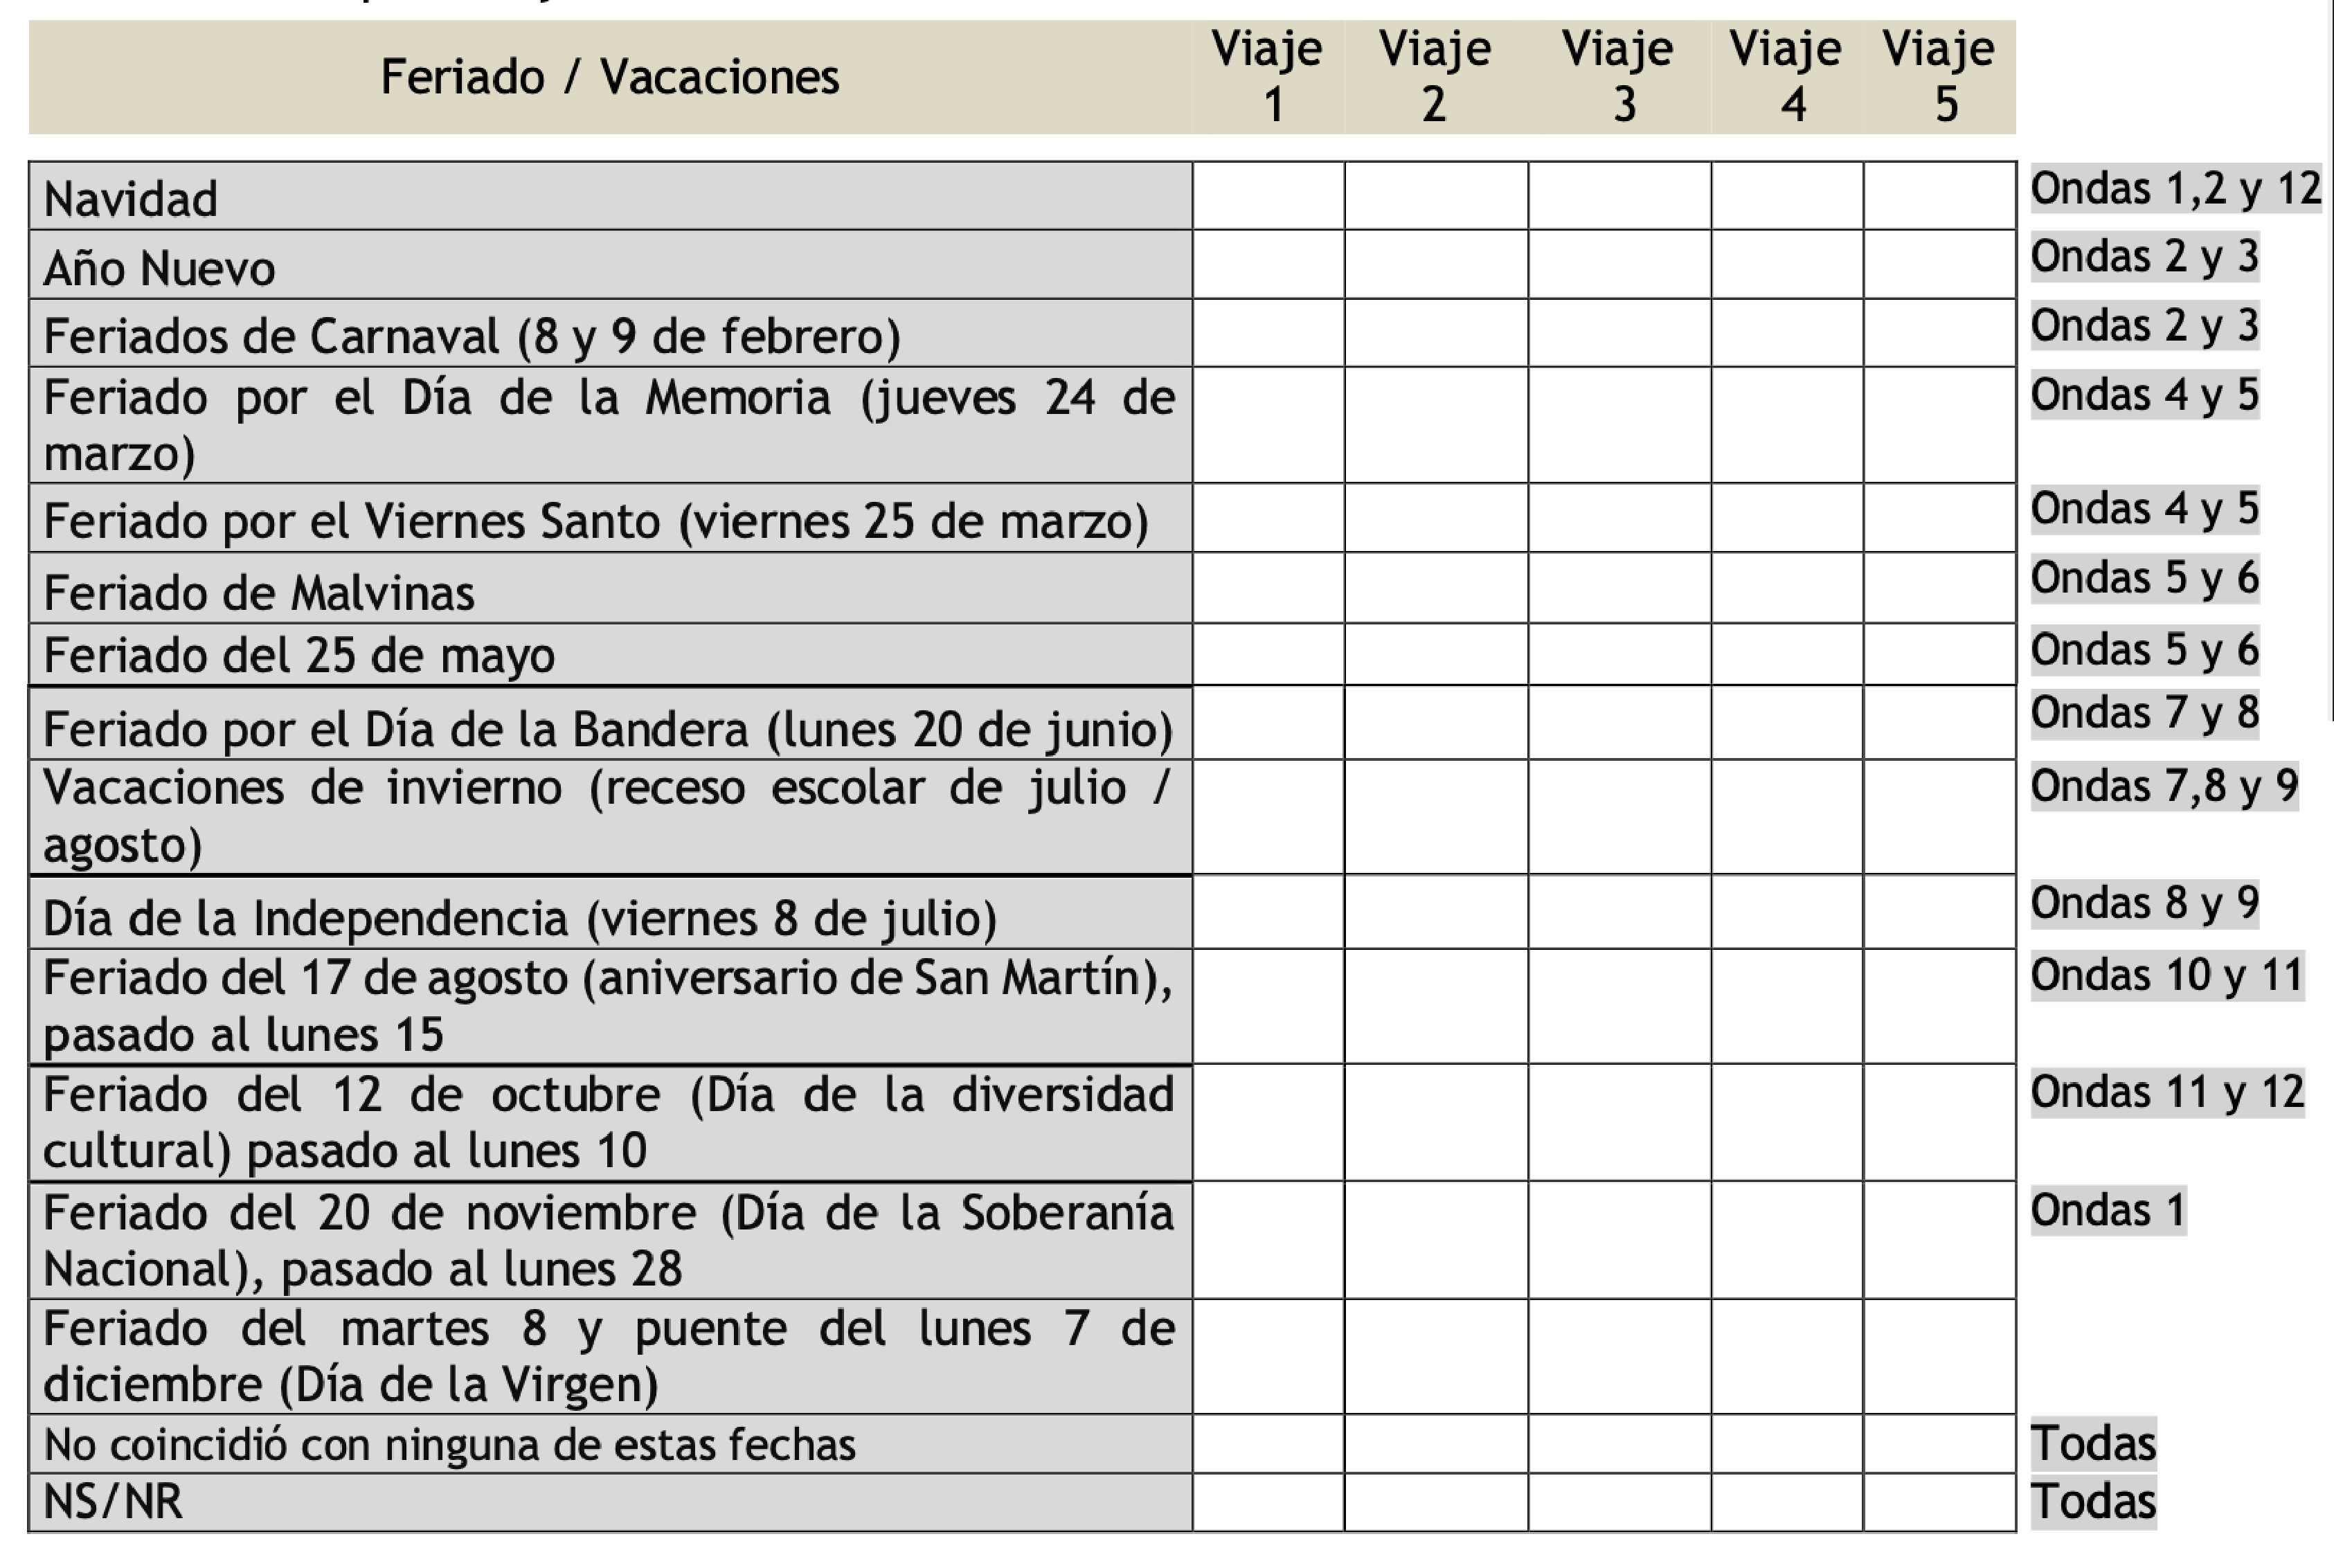
\includegraphics[width=1\linewidth]{imagenes/figura6-178} 

}

\end{figure}

\textbf{P406} ¿QUÉ INTEGRANTES DE SU HOGAR PARTICIPARON DEL VIAJE?

Marcar todas las opciones que correspondan. Dejar en blanco el espacio de los miembros que no viajaron.

\begin{figure}

{\centering 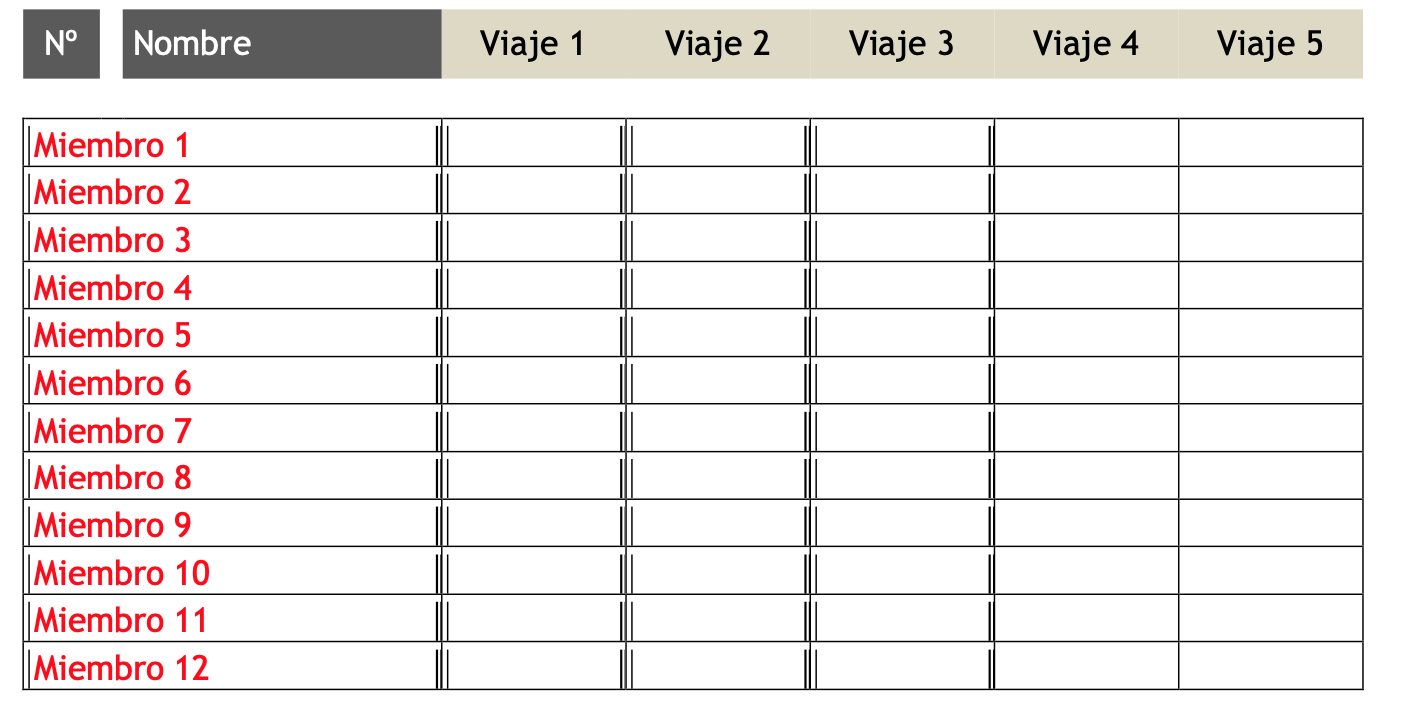
\includegraphics[width=1\linewidth]{imagenes/figura6-179} 

}

\end{figure}

\textbf{P407.1.} ¿CUÁL FUE LA DURACIÓN DEL VIAJE, DESDE QUE SALIERON HASTA QUE REGRESARON A SU HOGAR?
Anotar la cantidad de NOCHES o marcar el código de NS/NR.

\begin{figure}

{\centering 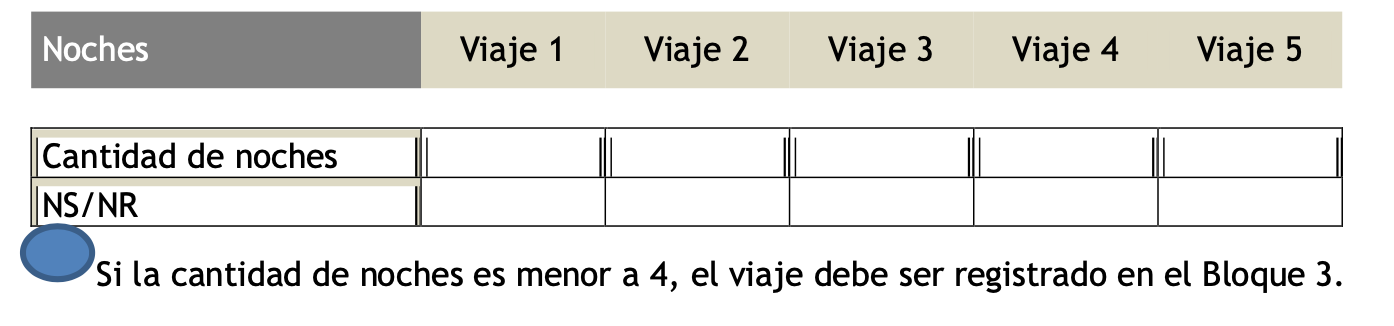
\includegraphics[width=1\linewidth]{imagenes/figura6-180} 

}

\end{figure}

\textbf{P409} ¿QUÉ MEDIO DE TRANSPORTE UTILIZARON PARA IR HASTA ALLÁ?

Marque una sola opción.

\begin{figure}

{\centering 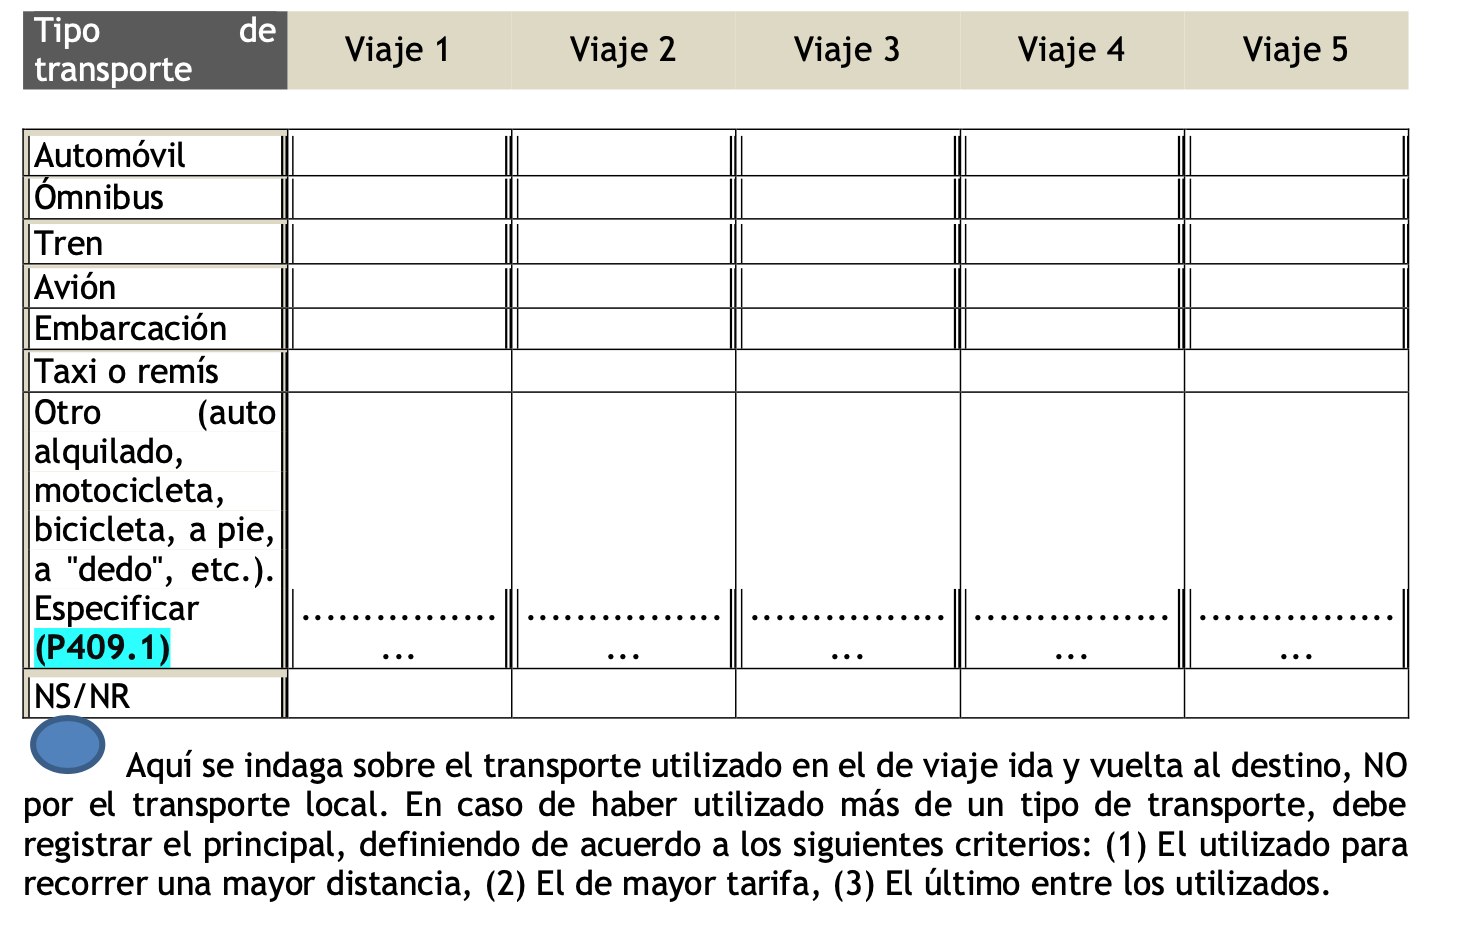
\includegraphics[width=1\linewidth]{imagenes/figura6-181} 

}

\end{figure}

\textbf{P410.1}¿CUÁL FUE EL MOTIVO DEL VIAJE?

Marque una sola opción

\begin{figure}

{\centering 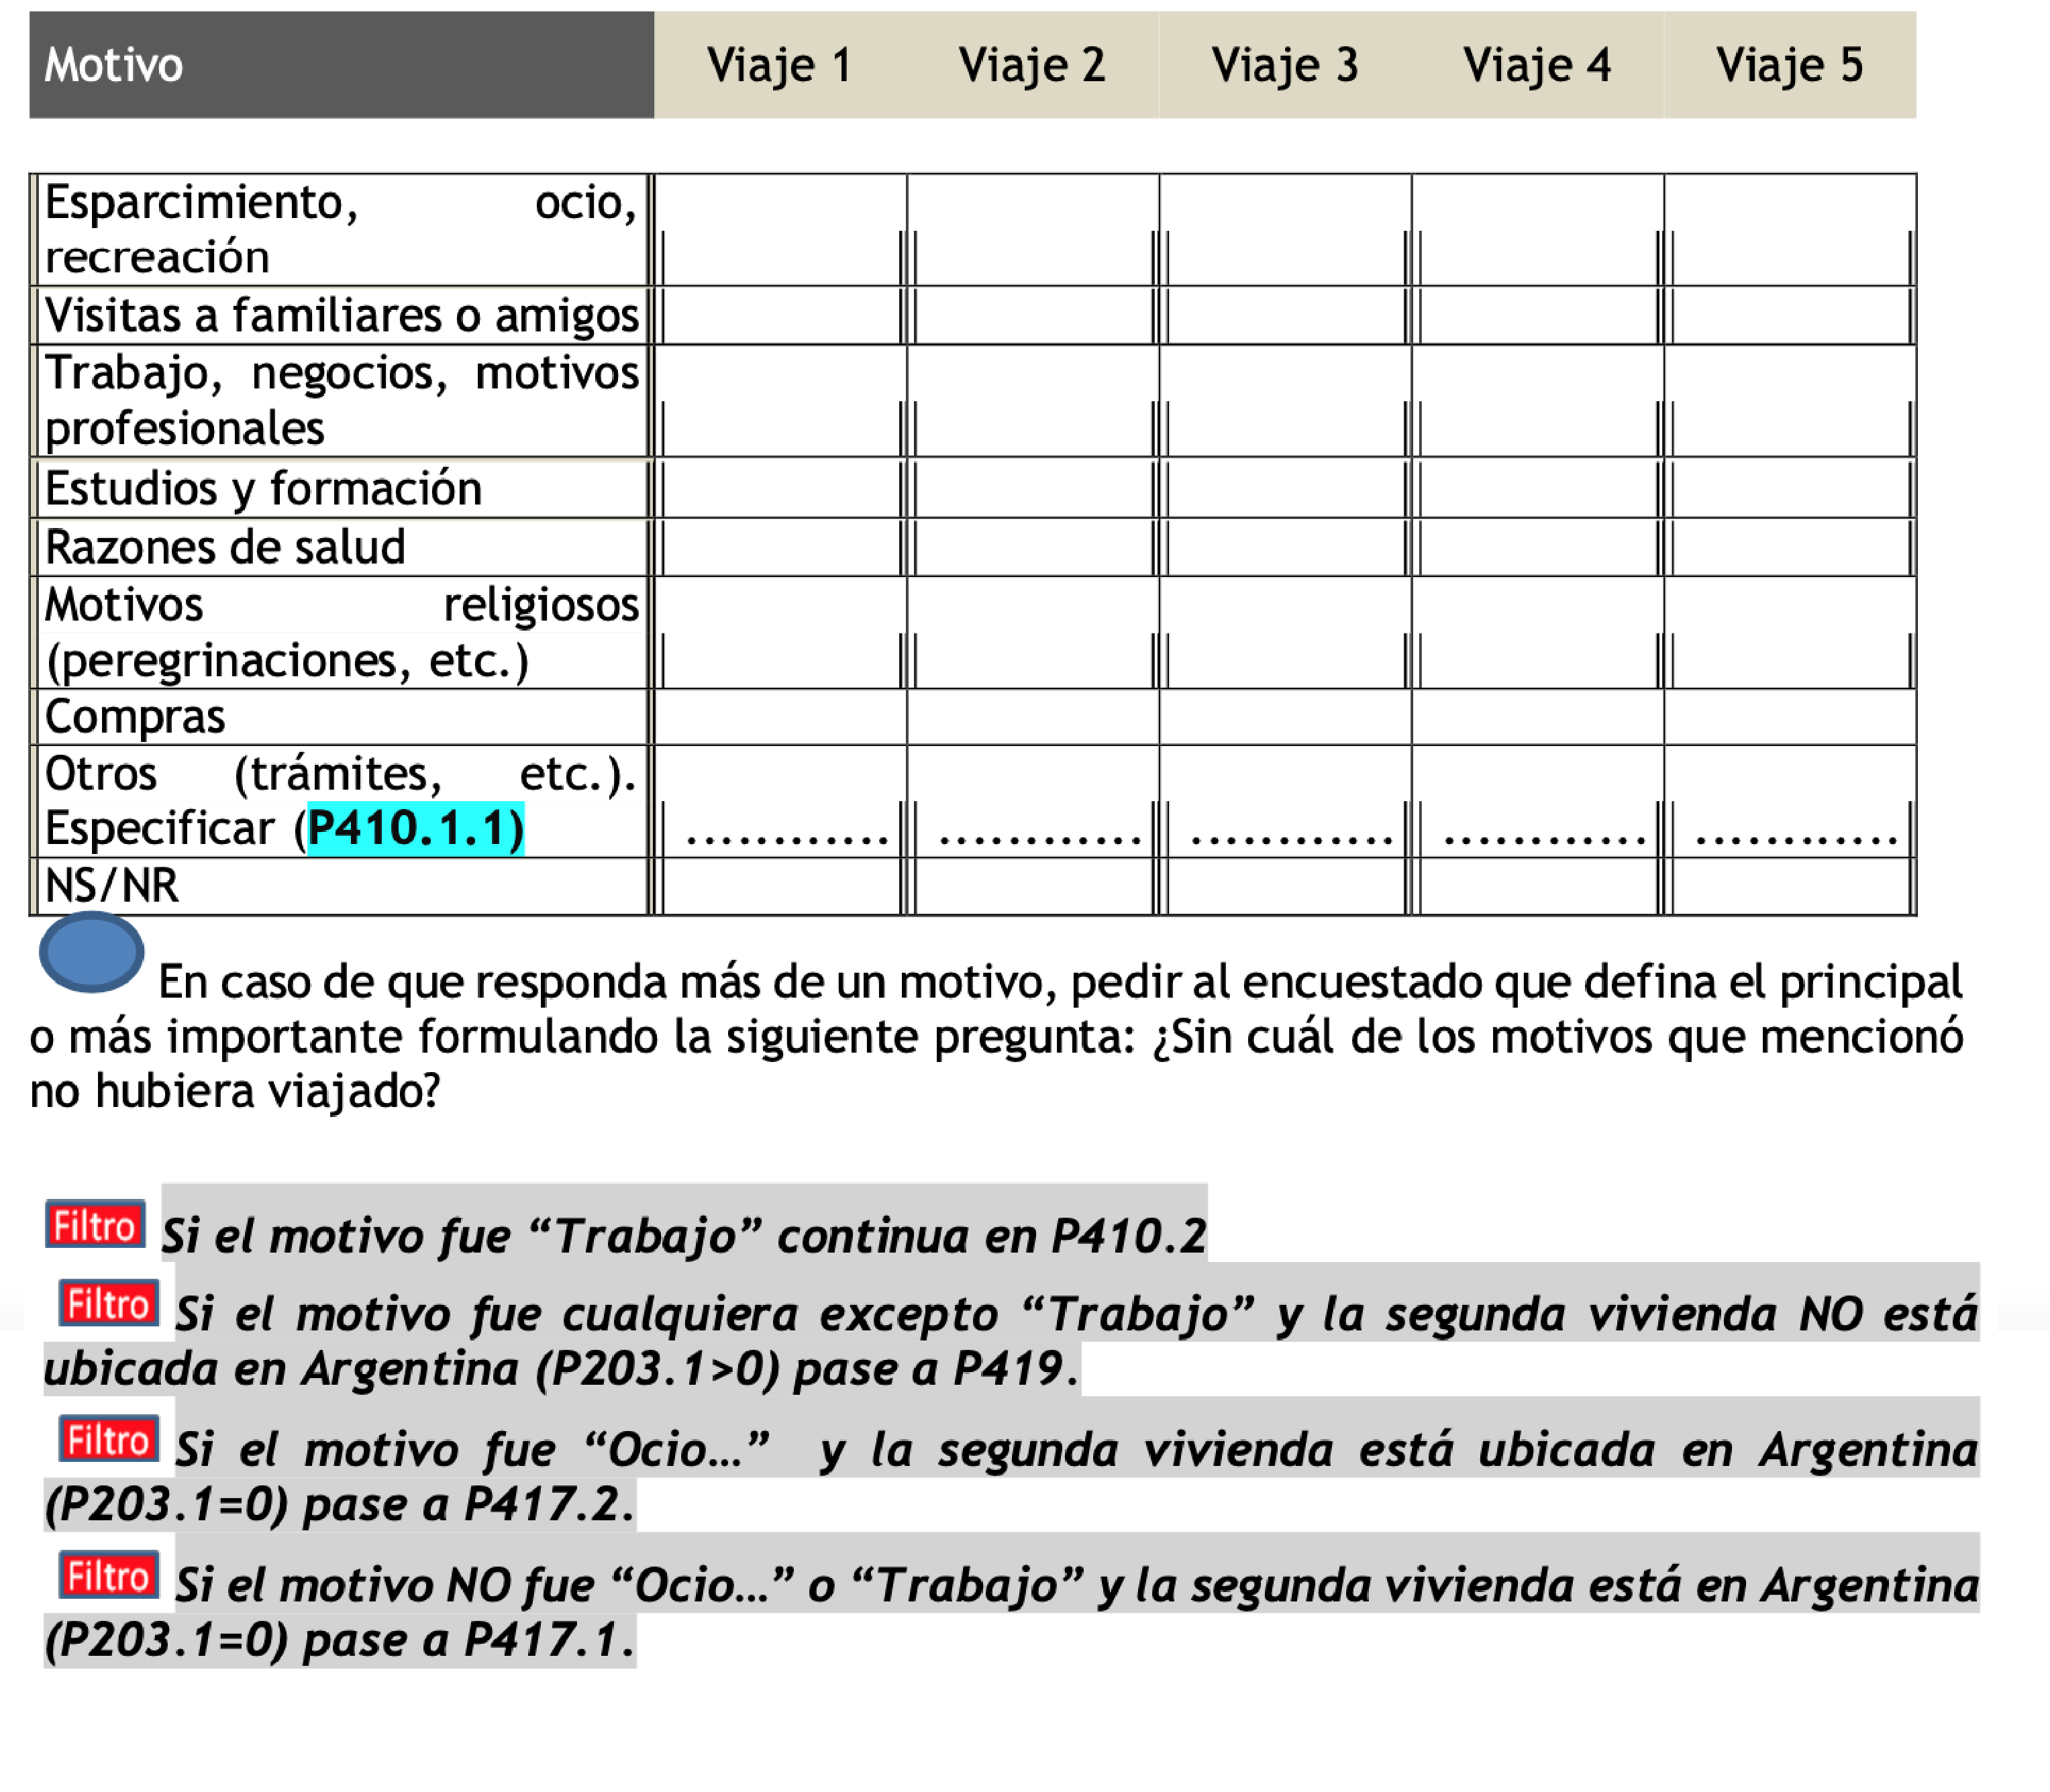
\includegraphics[width=1\linewidth]{imagenes/figura6-182} 

}

\end{figure}

\textbf{P410.2} ¿EL TRABAJO REALIZADO FUE COMO EMPLEADO DE UNA EMPRESA DEL LUGAR DE DESTINO?

¿EL DESPLAZAMIENTO O TRASLADO AL LUGAR DE DESTINO FORMÓ PARTE DE SU OFICIO (AZAFATA, VIAJANTE, CHOFER, TRANSPORTISTA, ETC.)?

Realizar la primera pregunta, si responde que no formular la siguiente. Marcar ``Si'' cuando responda afirmativamente a cualquiera de las dos preguntas.

\begin{figure}

{\centering 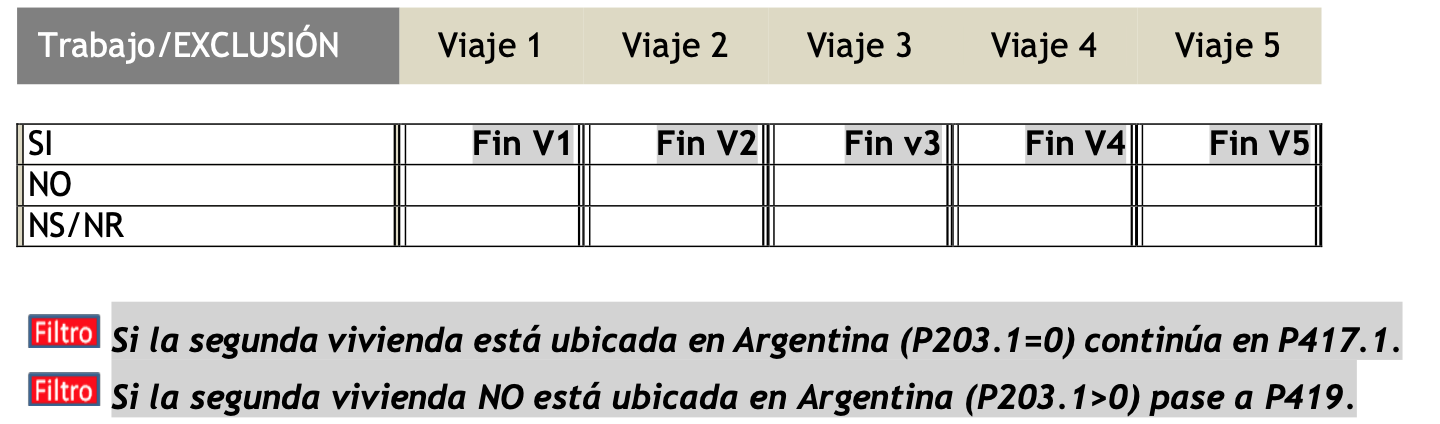
\includegraphics[width=1\linewidth]{imagenes/figura6-183} 

}

\end{figure}

\textbf{P417.1.} PESE A NO HACER ESTE VIAJE POR ESPARCIMIENTO, ¿EN ESTE VIAJE REALIZARON ALGUNA ACTIVIDAD TURÍSTICA O RECREATIVA COMO VISITAR ATRACTIVOS NATURALES O HISTÓRICOS, PRACTICAR DEPORTES NO CONVENCIONALES, IR A LA PLAYA, AL CINE, AL CASINO, U OTRAS ACTIVIDADES SIMILARES?

\begin{figure}

{\centering 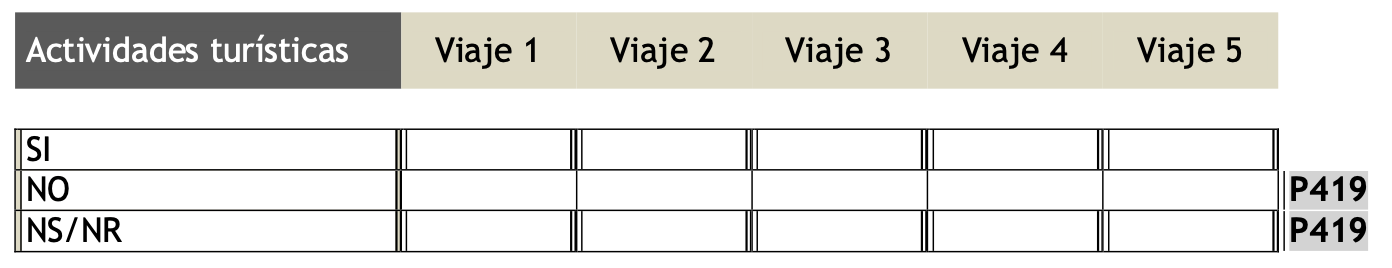
\includegraphics[width=1\linewidth]{imagenes/figura6-184} 

}

\end{figure}

\textbf{P417.2.} ¿CUÁLES DE LAS SIGUIENTES ACTIVIDADES TURÍSTICAS REALIZARON EN ESTE VIAJE? NO IMPORTA SI EN ELLAS PARTICIPARON TODOS O ALGUNO/S DE USTEDES
Leer una a una las opciones y esperar a que el entrevistado responda antes de pasar a la siguiente. Anotar en cada una alguno de los siguientes códigos: Si=1, No=2, NS/NR=9.

\begin{figure}

{\centering 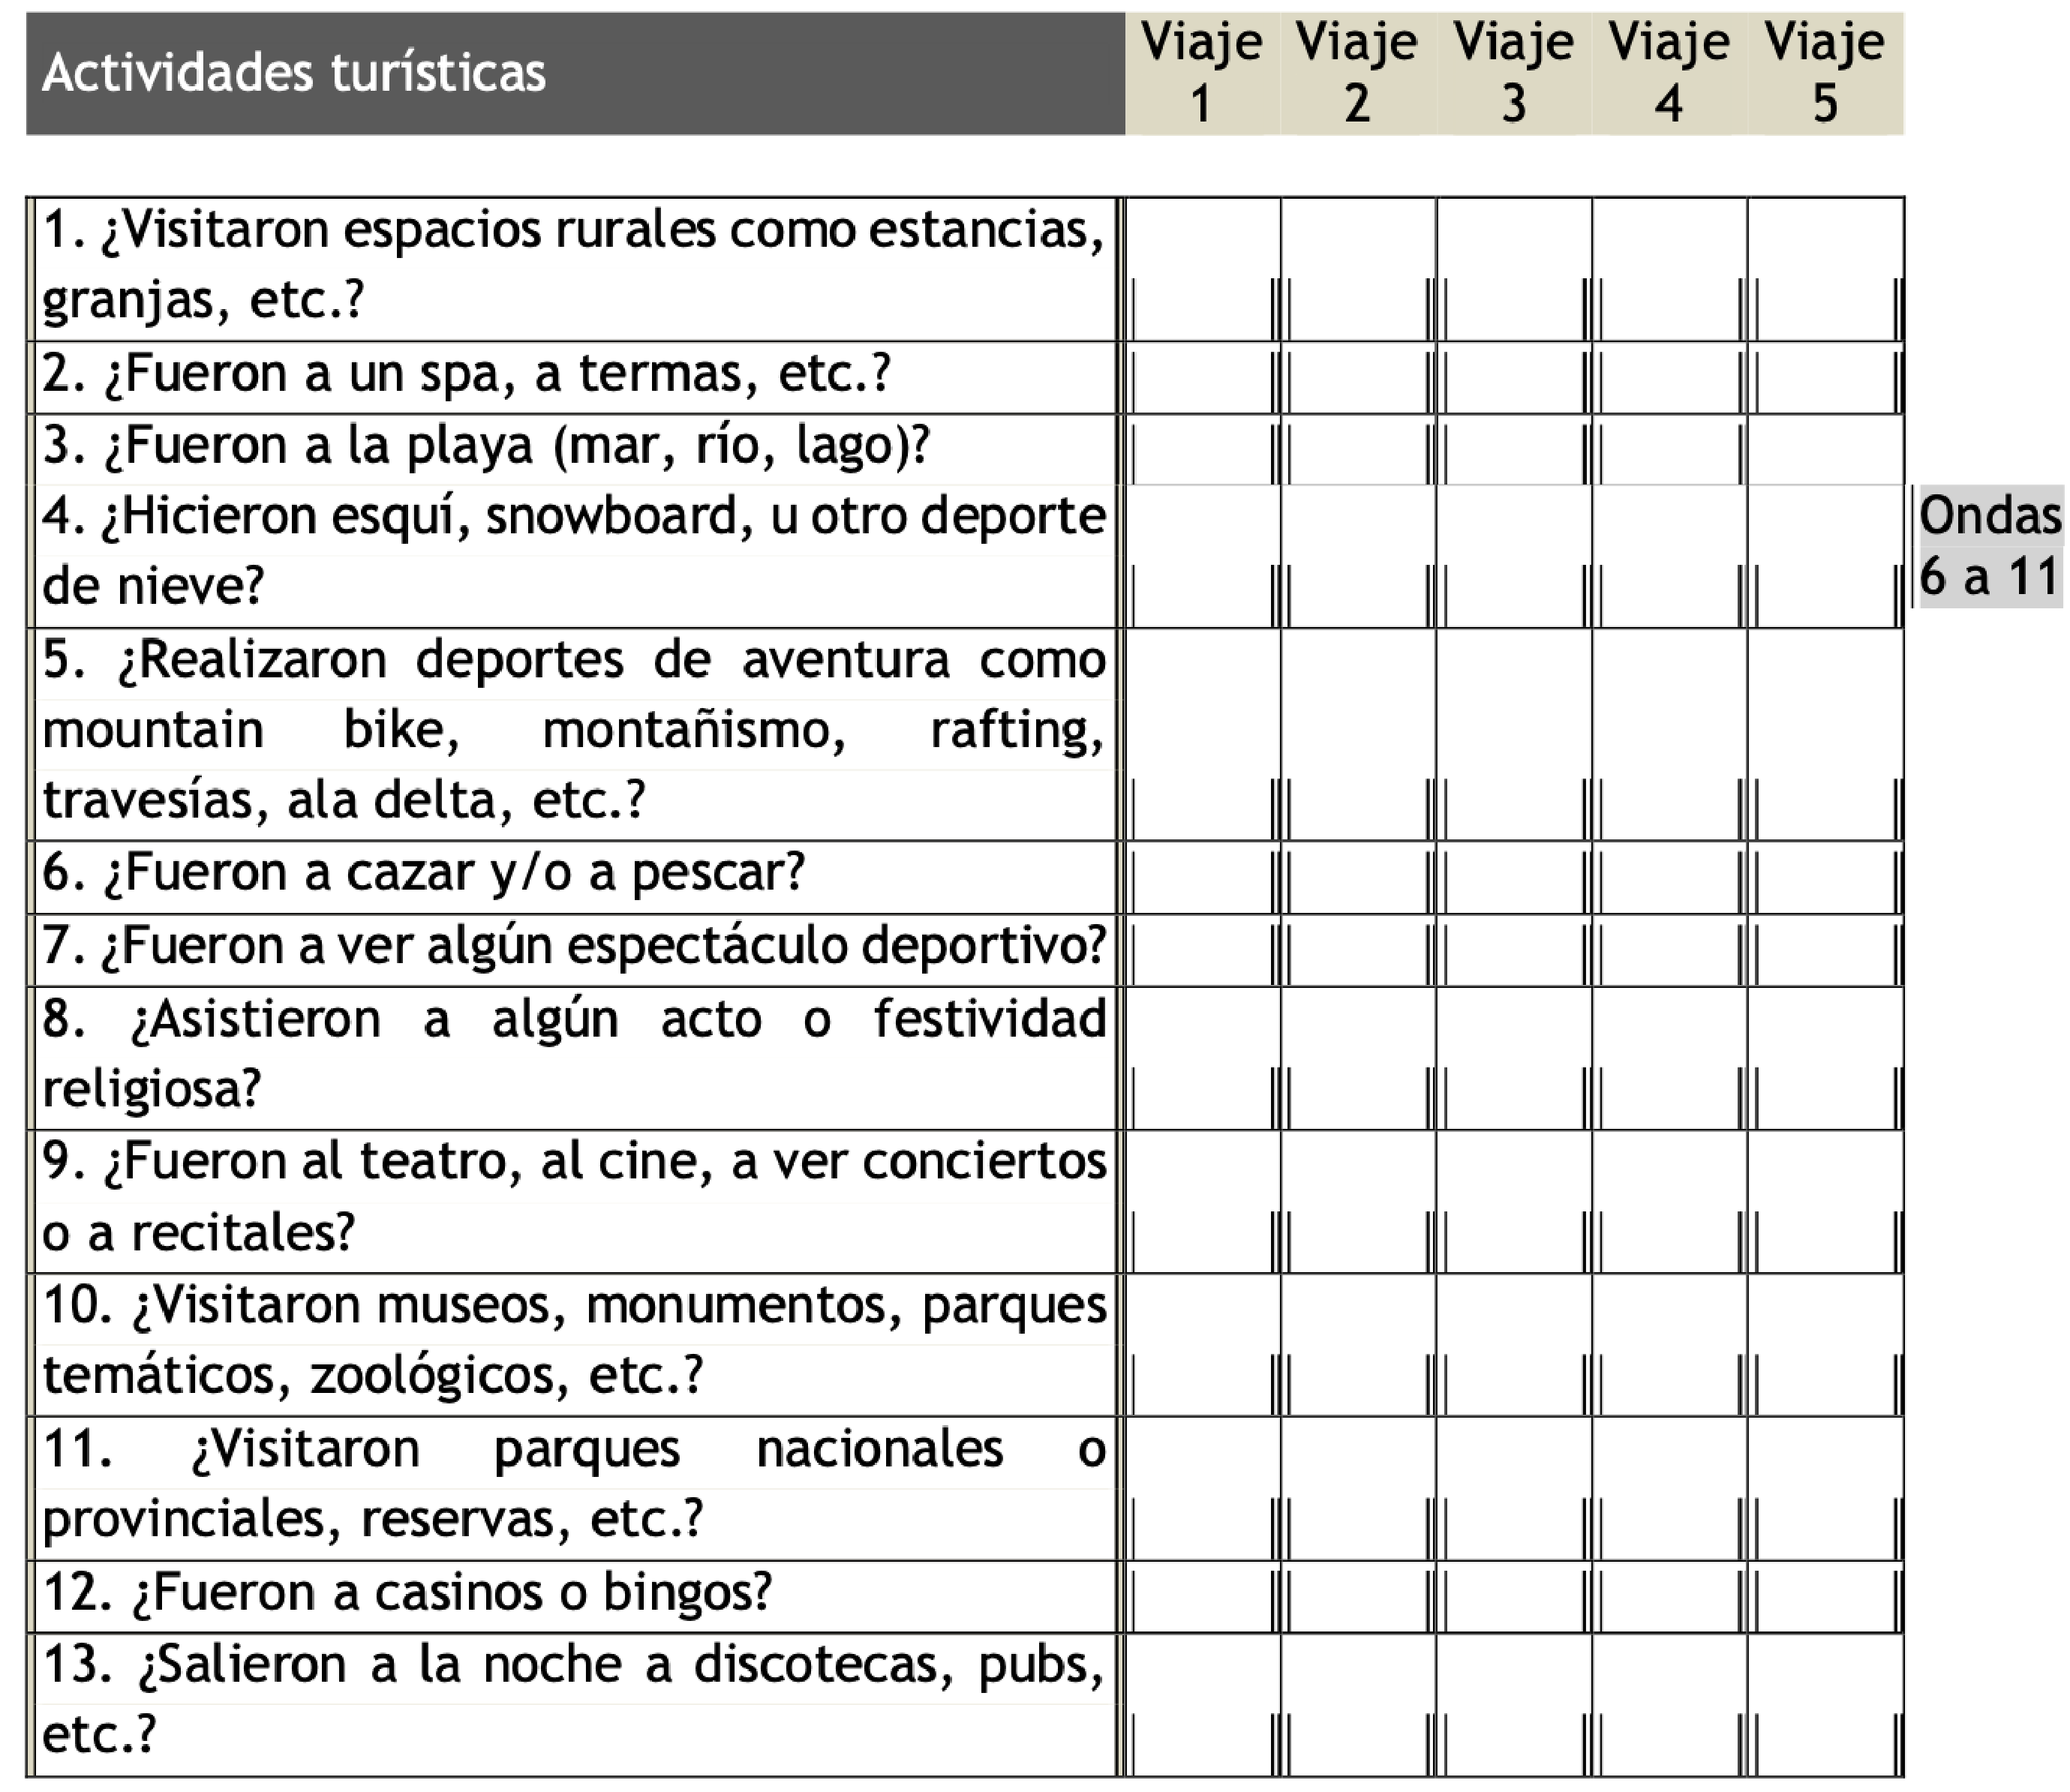
\includegraphics[width=1\linewidth]{imagenes/figura6-185} 

}

\end{figure}

\textbf{P419} ¿LOS GASTOS DEL VIAJE FUERON PAGADOS TOTALMENTE POR EL HOGAR?

\begin{figure}

{\centering 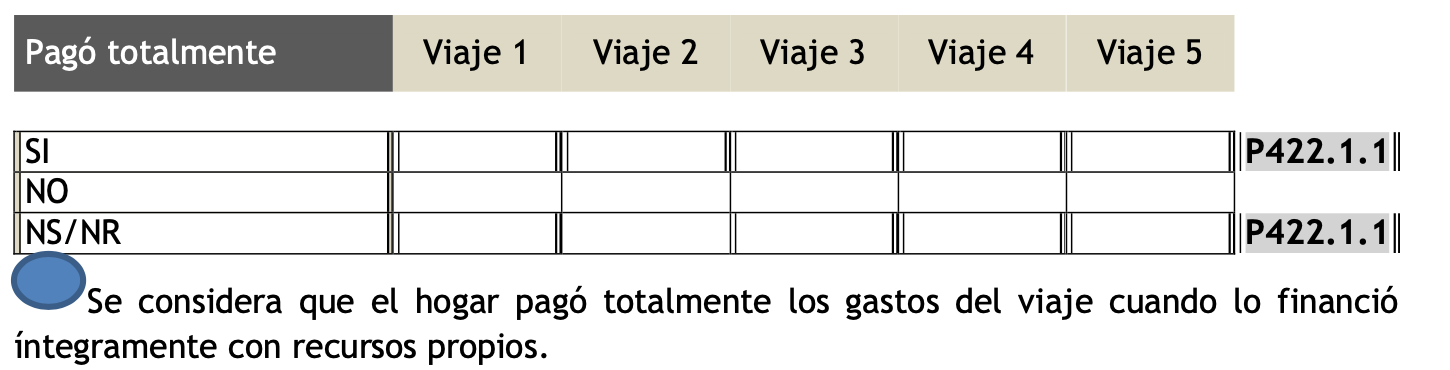
\includegraphics[width=1\linewidth]{imagenes/figura6-186} 

}

\end{figure}

\textbf{P420} ¿DE QUÉ PARTE DE LOS GASTOS SE HIZO CARGO EL HOGAR?
Marque una sola opción

\begin{figure}

{\centering 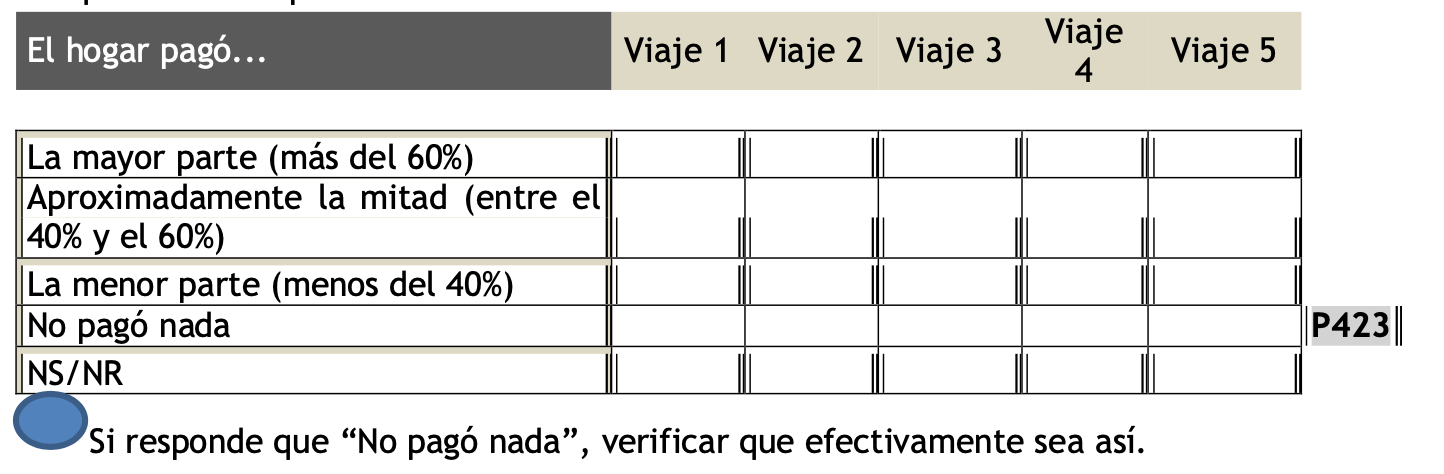
\includegraphics[width=1\linewidth]{imagenes/figura6-187} 

}

\end{figure}

\textbf{P422.1.1} APROXIMADAMENTE, ¿CUÁNTO GASTARON EN TOTAL EN EL VIAJE, INCLUYENDO
LOS GASTOS DE TODOS LOS MIEMBROS DEL HOGAR EN TRANSPORTE, COMIDAS, ETC.)?

\begin{figure}

{\centering 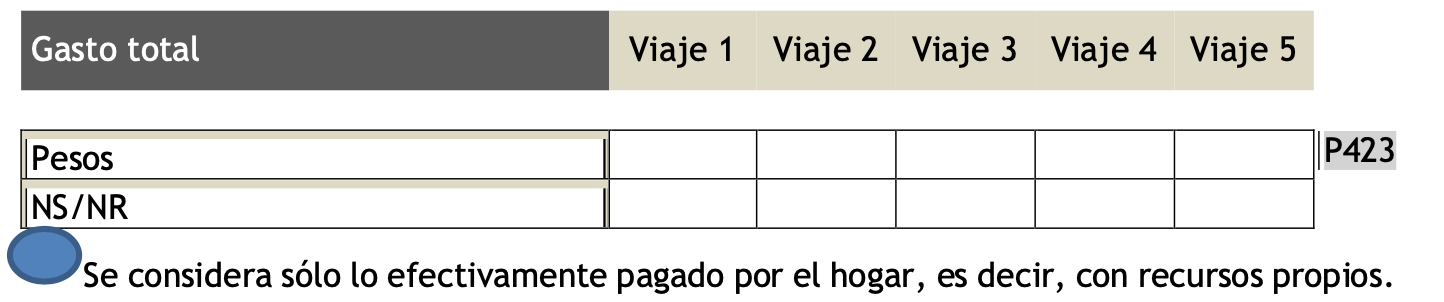
\includegraphics[width=1\linewidth]{imagenes/figura6-188} 

}

\end{figure}

\textbf{P422.2.4.} ¿PODRÍA DECIRME EN CUÁL DE LOS SIGUIENTES TRAMOS CREE QUE SE UBICA EL GASTO TOTAL DEL VIAJE PAGADO POR EL HOGAR?
Leer las opciones listadas y marcar la que señale el entrevistado.

\begin{figure}

{\centering 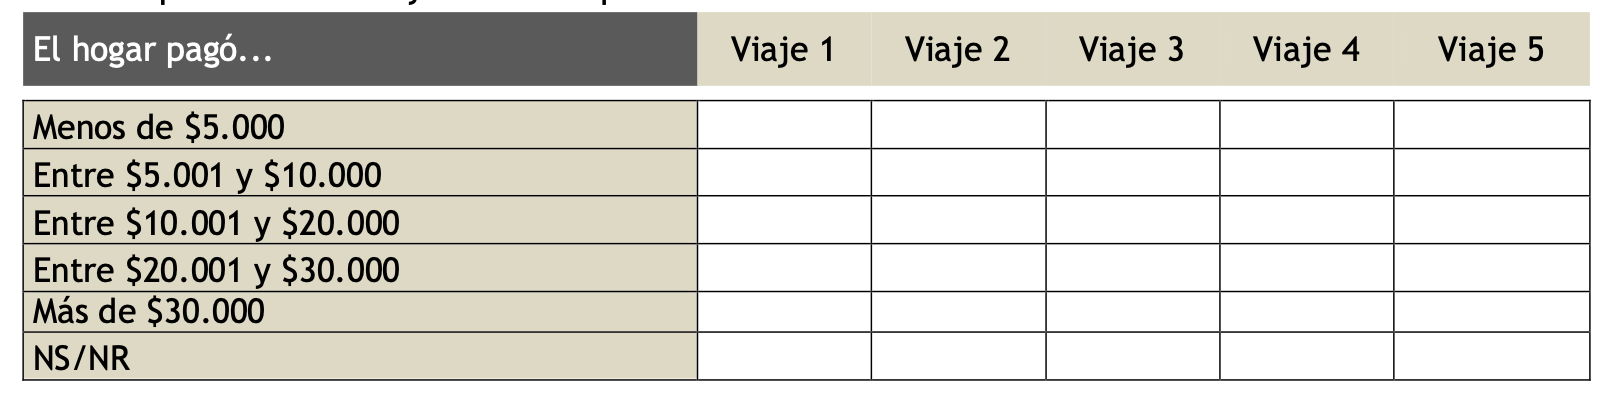
\includegraphics[width=1\linewidth]{imagenes/figura6-189} 

}

\end{figure}

\textbf{P423.} OBSERVACIONES REFERIDAS AL VIAJE
Completar sólo en caso de ser necesario.

\begin{figure}

{\centering 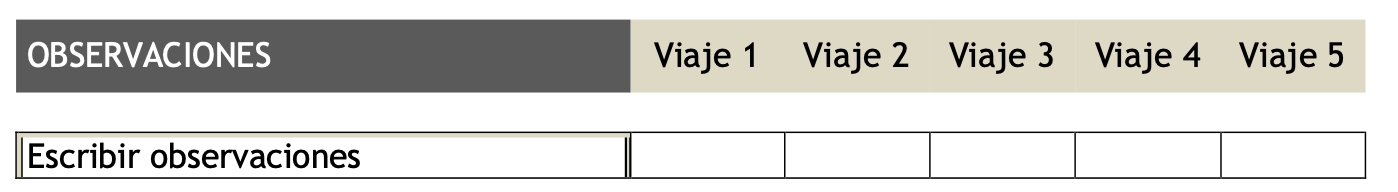
\includegraphics[width=1\linewidth]{imagenes/figura6-190} 

}

\end{figure}

\hypertarget{bloque-5.-visitas-de-un-duxeda-a-segundas-viviendas.}{%
\subsection{Bloque 5. Visitas de un día a segundas viviendas.}\label{bloque-5.-visitas-de-un-duxeda-a-segundas-viviendas.}}

\textbf{P501.} ¿EN LOS MESES DE \textbf{MES 1 y MES 2}, UD. O ALGÚN INTEGRANTE DEL HOGAR FUERON A PASAR EL DÍA, SIN QUEDARSE A DORMIR, A ESTA / ALGUNAS DE ESTAS VIVIENDA/S?

\begin{figure}

{\centering \includegraphics[width=1\linewidth]{imagenes/figura6-191} 

}

\end{figure}

\textbf{P503.2} ¿FUERON A PASAR ALGÚN DÍA A LA VIVIENDA UBICADA EN \ldots\ldots{}
Indague por cada segunda vivienda de la que dispone el hogar

\begin{figure}

{\centering \includegraphics[width=1\linewidth]{imagenes/figura6-192} 

}

\end{figure}

\textbf{P504.2.} ¿CUÁNTAS VECES FUERON A PASAR EL DÍA EN LA VIVIENDA EN \textbf{MES 1 Y CUÁNTAS EN MES 2}?

Anotar la cantidad. Si en uno de los meses no realizaron viajes registrar 0 (cero). Si tiene más de una segunda vivienda, preguntar por cada una de ellas.

\begin{figure}

{\centering \includegraphics[width=1\linewidth]{imagenes/figura6-193} 

}

\end{figure}

\textbf{P505.2.} ¿ALGUNO DE ESOS DÍAS COINCIDIÓ CON\ldots.

Leer todas las opciones. Anotar en cada una alguno de los siguientes códigos: Si=1, No=2, NS/NR=9.

\begin{figure}

{\centering \includegraphics[width=1\linewidth]{imagenes/figura6-194} 

}

\end{figure}

\textbf{P506} ¿QUÉ INTEGRANTES DE SU HOGAR FUERON ESE DÍA?

Marcar todas las opciones que correspondan. Dejar en blanco el espacio de los miembros que no viajaron.

\begin{figure}

{\centering \includegraphics[width=1\linewidth]{imagenes/figura6-195} 

}

\end{figure}

\textbf{P509} ¿QUÉ MEDIO DE TRANSPORTE UTILIZARON PARA IR HASTA ALLÁ?

Marque una sola opción.

\begin{figure}

{\centering \includegraphics[width=1\linewidth]{imagenes/figura6-196} 

}

\end{figure}

\textbf{P510.1} ¿CUÁL FUE EL MOTIVO POR EL QUE FUERON A PASAR EL DÍA A ESTA VIVIENDA?

Marque una sola opción.

\begin{figure}

{\centering \includegraphics[width=1\linewidth]{imagenes/figura6-197} 

}

\end{figure}

\textbf{P510.2} ¿EL TRABAJO REALIZADO FUE COMO EMPLEADO DE UNA EMPRESA DEL LUGAR DE DESTINO?
¿EL DESPLAZAMIENTO O TRASLADO AL LUGAR DE DESTINO FORMÓ PARTE DE SU OFICIO (AZAFATA, VIAJANTE, CHOFER, TRANSPORTISTA, ETC.)?

Realizar la primera pregunta, si responde ``No'' formular la siguiente. Marcar ``Si'' cuando responda afirmativamente a cualquiera de las dos preguntas.

\begin{figure}

{\centering \includegraphics[width=1\linewidth]{imagenes/figura6-198} 

}

\end{figure}

\textbf{P517.1.} ¿EN ESTA VISITA REALIZARON ALGUNA ACTIVIDAD TURÍSTICA O RECREATIVA COMO VISITAR ATRACTIVOS NATURALES O HISTÓRICOS, PRACTICAR DEPORTES NO CONVENCIONALES, IR A LA PLAYA, AL CINE, AL CASINO, U OTRAS ACTIVIDADES SIMILARES?

\begin{figure}

{\centering \includegraphics[width=1\linewidth]{imagenes/figura6-199} 

}

\end{figure}

\textbf{P517.2.} ¿CUÁLES DE LAS SIGUIENTES ACTIVIDADES TURÍSTICAS REALIZARON EN ESTA VISITA DE UN DÍA? NO IMPORTA SI EN ELLAS PARTICIPARON TODOS O ALGUNO/S DE USTEDES

Leer una a una las opciones y esperar a que el entrevistado responda antes de pasar a la siguiente. Anotar en cada una alguno de los siguientes códigos: Si=1, No=2, NS/NR=9.

\begin{figure}

{\centering \includegraphics[width=1\linewidth]{imagenes/figura6-200} 

}

\end{figure}

\textbf{P519} ¿LOS GASTOS QUE TUVIERON ESE DÍA FUERON PAGADOS TOTALMENTE POR EL HOGAR?

\begin{figure}

{\centering \includegraphics[width=1\linewidth]{imagenes/figura6-201} 

}

\end{figure}

\textbf{P520} ¿DE QUÉ PARTE DE LOS GASTOS SE HIZO CARGO EL HOGAR?

Marque una sola opción.

\begin{figure}

{\centering \includegraphics[width=1\linewidth]{imagenes/figura6-202} 

}

\end{figure}

\textbf{P522.1.1} APROXIMADAMENTE, ¿CUÁNTO GASTARON EN TOTAL POR IR A PASAR EL DÍA, INCLUYENDO LOS GASTOS DE TODOS LOS MIEMBROS DEL HOGAR EN TRANSPORTE, COMIDAS, ETC.?

\begin{figure}

{\centering \includegraphics[width=1\linewidth]{imagenes/figura6-203} 

}

\end{figure}

\textbf{P522.1.2.5.} ¿PODRÍA DECIRME EN CUÁL DE LOS SIGUIENTES TRAMOS CREE QUE SE UBICA EL GASTO TOTAL DE ESE DÍA PAGADO POR EL HOGAR?

Leer las opciones listadas y marcar la que señale el entrevistado.

\begin{figure}

{\centering \includegraphics[width=1\linewidth]{imagenes/figura6-204} 

}

\end{figure}

\textbf{P523.} OBSERVACIONES REFERIDAS A LA VISITA DE UN DÍA

Completar sólo en caso de ser necesario.

\begin{figure}

{\centering \includegraphics[width=1\linewidth]{imagenes/figura6-205} 

}

\end{figure}

\hypertarget{bloque-6.-viajes-no-reiterados-en-argentina.}{%
\subsection{Bloque 6. Viajes no reiterados en argentina.}\label{bloque-6.-viajes-no-reiterados-en-argentina.}}

\textbf{``AHORA LE VOY A PREGUNTAR POR VIAJES O EXCURSIONES QUE HAYAN REALIZADO EN LOS MESES DE MES 1 Y MES 2 POR CUALQUIER MOTIVO (OCIO, VACACIONES, VISITAS A FAMILIARES O AMIGOS, TRABAJO O CUALQUIER OTRO)''}

\textbf{P601.} ¿EN \textbf{MES 1 y MES 2} VIAJARON A ALGUN LUGAR DE ARGENTINA UBICADO A MÁS DE 20/40 KM, DE DONDE VIVEN PASANDO ALLÍ AL MENOS UNA NOCHE?

\begin{figure}

{\centering \includegraphics[width=1\linewidth]{imagenes/figura6-206} 

}

\end{figure}

No importa si viajaron todos, algunos o sólo uno de los miembros del hogar.
Los viajes pueden haber sido realizados por cualquier motivo (no mencionar la palabra turismo). Insistir con distintas posibilidades por las que pudieron haber hecho viajes, así como con las fechas claves del periodo de referencia.
Si dicen que hicieron algún viaje, confirmar los aspectos que definen que efectivamente se trata de un viaje a registrar en este bloque:
-La ciudad o localidad a la que fueron debe estar a más de 20/40 KM de donde reside el hogar contactado y estar en Argentina.
-Deben haber dormido al menos una noche en cualquier tipo de alojamiento.
-Al menos uno de los viajes tiene que tener como fecha de regreso uno de los meses de referencia.
-Si viajaron a un mismo destino con frecuencia semanal, no debe considerarse como viaje porque el destino forma parte del entorno habitual del hogar.
-Si se detecta que hicieron 3 o más viajes similares a un mismo destino (sin llegar a hacerlo con frecuencia semanal), ellos no deben ser registrados aquí sino en el bloque 8. Si además de esos viajes hicieron otros viajes no reiterados marcar sí y continuar (sin olvidar de registrar los viajes reiterados en el bloque 8). Si solo hicieron viajes reiterados, marcar no y pasar al bloque siguiente.

\textbf{P602} ¿CUÁNTOS VIAJES EN ARGENTINA HICIERON EN \textbf{MES 1 Y MES 2}?

Anotar la cantidad de viajes con fecha de regreso en los meses incluidos en el bimestre de referencia.

\begin{figure}

{\centering \includegraphics[width=1\linewidth]{imagenes/figura6-207} 

}

\end{figure}

\textbf{P603.1} ¿CUÁL FUE LA PROVINCIA Y LA CIUDAD QUE VISITARON EN CADA VIAJE?
Anotar el nombre en el espacio en blanco correspondiente. Si no sabe o no recuerda, escribir NS/NR.

\begin{figure}

{\centering \includegraphics[width=1\linewidth]{imagenes/figura6-208} 

}

\end{figure}

\textbf{P603.1.4} EN ESTE VIAJE, ADEMÁS DE CIUDAD/LOCALIDAD ¿PASARON AL MENOS UNA NOCHE EN OTRA CIUDAD?

\begin{figure}

{\centering \includegraphics[width=1\linewidth]{imagenes/figura6-209} 

}

\end{figure}

\textbf{P603.1.5} ¿EN CUÁNTAS OTRAS CIUDADES SE ALOJARON AL MENOS UNA NOCHE?

Si NS/NR anotar 99.

\begin{figure}

{\centering \includegraphics[width=1\linewidth]{imagenes/figura6-210} 

}

\end{figure}

\textbf{P604.1.} ¿EL VIAJE FUE REALIZADO EN \textbf{MES 1 O MES 2}?

\begin{figure}

{\centering \includegraphics[width=1\linewidth]{imagenes/figura6-211} 

}

\end{figure}

\textbf{P605.1.} ¿ESTE VIAJE COINCIDIÓ CON\ldots{}

Leer todas las opciones y marcar una.

\begin{figure}

{\centering \includegraphics[width=1\linewidth]{imagenes/figura6-212} 

}

\end{figure}

\textbf{P606} ¿QUÉ INTEGRANTES DEL HOGAR PARTICIPARON DE ESTE VIAJE?

Marque todas las opciones que correspondan. Dejar en blanco el espacio de los miembros que no viajaron.

\begin{figure}

{\centering \includegraphics[width=1\linewidth]{imagenes/figura6-213} 

}

\end{figure}

\textbf{P607.1} ¿CUÁL FUE LA DURACIÓN DEL VIAJE, DESDE QUE SALIERON HASTA QUE REGRESARON A SU HOGAR?

Anotar la cantidad de NOCHES o marcar el código de NS/NR.

\begin{figure}

{\centering \includegraphics[width=1\linewidth]{imagenes/figura6-214} 

}

\end{figure}

\textbf{P608} ¿DÓNDE SE ALOJARON?

Marcar una sola opción.

\begin{figure}

{\centering \includegraphics[width=1\linewidth]{imagenes/figura6-215} 

}

\end{figure}

\textbf{P609} ¿QUÉ MEDIO DE TRANSPORTE UTILIZARON PARA IR HASTA ALLÁ?

Marque una sola opción.

\begin{figure}

{\centering \includegraphics[width=1\linewidth]{imagenes/figura6-216} 

}

\end{figure}

\textbf{P610.1} ¿CUÁL FUE EL MOTIVO DEL VIAJE?

Marque una sola opción

\begin{figure}

{\centering \includegraphics[width=1\linewidth]{imagenes/figura6-217} 

}

\end{figure}

\textbf{P610.2} ¿EL TRABAJO REALIZADO FUE COMO EMPLEADO DE UNA EMPRESA DEL LUGAR DE DESTINO?

¿EL DESPLAZAMIENTO O TRASLADO AL LUGAR DE DESTINO FORMÓ PARTE DE SU OFICIO (AZAFATA, VIAJANTE, CHOFER, TRANSPORTISTA, ETC.)?

Realizar la primera pregunta, si responde ``No'' formular la siguiente. Marcar ``Si'' cuando responda afirmativamente a cualquiera de las dos preguntas.

\begin{figure}

{\centering \includegraphics[width=1\linewidth]{imagenes/figura6-218} 

}

\end{figure}

\textbf{P611} ¿CONTRATARON UN PAQUETE TURÍSTICO PARA REALIZAR EL VIAJE?

\begin{figure}

{\centering \includegraphics[width=1\linewidth]{imagenes/figura6-219} 

}

\end{figure}

\textbf{P612} ¿QUÉ SERVICIOS INCLUYÓ EL PAQUETE TURÍSTICO?

Leer todas las opciones. Anotar en cada una alguno de los siguientes códigos: Si=1, No=2, NS/NR=9.

\begin{figure}

{\centering \includegraphics[width=1\linewidth]{imagenes/figura6-220} 

}

\end{figure}

\textbf{P613} ¿CON CUÁNTO TIEMPO DE ANTICIPACIÓN DECIDIERON REALIZAR EL VIAJE?

Esperar a que el encuestado responda. Si no lo hace, leer las opciones. Marcar una sola opción.

\begin{figure}

{\centering \includegraphics[width=1\linewidth]{imagenes/figura6-221} 

}

\end{figure}

\textbf{P614}¿UTILIZARON INTERNET PARA CONSULTAR INFORMACIÓN O CONTRATAR SERVICIOS PARA SU VIAJE (SOBRE TRANSPORTE, ALOJAMIENTOS, ATRACTIVOS TURÍSTICOS DEL DESTINO, ETC.)?

\begin{figure}

{\centering \includegraphics[width=1\linewidth]{imagenes/figura6-222} 

}

\end{figure}

\textbf{P615.} POR FAVOR, DÍGAME SI PARA ESTE VIAJE, POR MEDIO DE INTERNET\ldots{}

Leer todas las opciones. Anotar en cada una alguno de los siguientes códigos: Si=1, No=2, NS/NR=9.

\begin{figure}

{\centering \includegraphics[width=1\linewidth]{imagenes/figura6-223} 

}

\end{figure}

\textbf{P616.1.} Por favor, dígame si cada una de las razones que le voy a leer influyó o no en su decisión de visitar Ciudad/Localidad:

Cada fila es una pregunta independiente que debe ser respondida por sí o no. Si la respuesta es SI se marca, si es NO o NS/NR se deja vacío

\begin{figure}

{\centering \includegraphics[width=1\linewidth]{imagenes/figura6-224} 

}

\end{figure}

\textbf{P616.2.} Algún integrante del hogar que participó de este viaje a Ciudad/Localidad, ¿había viajado allí antes? ¿Cuándo fue la última vez que viajó/viajaron allí?

\begin{figure}

{\centering \includegraphics[width=1\linewidth]{imagenes/figura6-225} 

}

\end{figure}

\textbf{P617.1.} PESE A NO SER UN VIAJE QUE HICIERON POR ESPARCIMIENTO ¿EN ESTE VIAJE REALIZARON ALGUNA ACTIVIDAD TURÍSTICA O RECREATIVA COMO VISITAR ATRACTIVOS NATURALES O HISTÓRICOS, PRACTICAR DEPORTES NO CONVENCIONALES, IR A LA PLAYA, AL CINE, AL CASINO, U OTRAS ACTIVIDADES SIMILARES?

\begin{figure}

{\centering \includegraphics[width=1\linewidth]{imagenes/figura6-226} 

}

\end{figure}

\textbf{P617.2} ¿CUÁLES DE LAS SIGUIENTES ACTIVIDADES TURÍSTICAS REALIZARON EN ESTE VIAJE? NO IMPORTA SI EN ELLAS PARTICIPARON TODOS O ALGUNO/S DE USTEDES.

Leer una a una las opciones y esperar a que el entrevistado responda antes de pasar a la siguiente. Anotar en cada una alguno de los siguientes códigos: Si=1, No=2, NS/NR=9.

\begin{figure}

{\centering \includegraphics[width=1\linewidth]{imagenes/figura6-227} 

}

\end{figure}

\textbf{P618.} DE ACUERDO A LO QUE USTED ESPERABA, POR FAVOR, CALIFIQUE DE 1 A 10 PUNTOS LOS SIGUIENTES ASPECTOS DE SU VIAJE:

Leer cada uno de los aspectos y esperar a que el encuestado otorgue una calificación, luego pasar al siguiente. Registrar valor de 1 (pésimo) a 10 (excelente). Si no utilizó, anotar 88; si NS/NR, anotar 99.

\begin{figure}

{\centering \includegraphics[width=1\linewidth]{imagenes/figura6-228} 

}

\end{figure}

\textbf{P619} ¿LOS GASTOS DEL VIAJE FUERON PAGADOS TOTALMENTE POR EL HOGAR?

\begin{figure}

{\centering \includegraphics[width=1\linewidth]{imagenes/figura6-229} 

}

\end{figure}

\textbf{P620} ¿DE QUÉ PARTE DE LOS GASTOS SE HIZO CARGO EL HOGAR?

Marque una sola opción

\begin{figure}

{\centering \includegraphics[width=1\linewidth]{imagenes/figura6-230} 

}

\end{figure}

\textbf{P621.1} ¿CUÁNTO GASTARON EN EL PAQUETE TURÍSTICO?

Si NS/NR marcar el código. Si el hogar no pagó el PT, anotar 0 (sólo válido en los casos que el hogar haya pagado sólo una parte de los gastos del viaje).

\begin{figure}

{\centering \includegraphics[width=1\linewidth]{imagenes/figura6-231} 

}

\end{figure}

\textbf{P622.1.1} APROXIMADAMENTE, ¿CUÁNTO GASTARON EN TOTAL EN EL VIAJE, INCLUYENDO LOS GASTOS DE TODOS LOS MIEMBROS DEL HOGAR EN TRANSPORTE, ALOJAMIENTO, COMIDAS, EXCURSIONES, ETC.?

Si utilizaron Paquete, incluirlo como ejemplo dentro de la pregunta. Si NS/NR marque el código.

\begin{figure}

{\centering \includegraphics[width=1\linewidth]{imagenes/figura6-232} 

}

\end{figure}

\textbf{P622.1.2.6.} ¿PODRÍA DECIRME EN CUÁL DE LOS SIGUIENTES TRAMOS CREE QUE SE UBICA EL GASTO TOTAL DEL VIAJE PAGADO POR EL HOGAR?

Leer las opciones listadas y marcar la que señale el entrevistado.

\begin{figure}

{\centering \includegraphics[width=1\linewidth]{imagenes/figura6-233} 

}

\end{figure}

\textbf{P623.} OBSERVACIONES REFERIDAS AL VIAJE

Completar sólo en caso de ser necesario.

\begin{figure}

{\centering \includegraphics[width=1\linewidth]{imagenes/figura6-234} 

}

\end{figure}

\hypertarget{bloque-7.-viajes-no-reiterados-al-extranjero.}{%
\subsection{Bloque 7. Viajes no reiterados al extranjero.}\label{bloque-7.-viajes-no-reiterados-al-extranjero.}}

\textbf{P701.} ¿EN MES 1 y MES 2 VIAJARON A ALGUN PAÍS EXTRANJERO?

\begin{figure}

{\centering \includegraphics[width=1\linewidth]{imagenes/figura6-235} 

}

\end{figure}

\textbf{P702} ¿CUÁNTOS VIAJES AL EXTERIOR HICIERON EN MES 1 Y MES 2?

Anotar la cantidad de viajes con fecha de regreso en los meses incluidos en el bimestre de referencia.

\begin{figure}

{\centering \includegraphics[width=1\linewidth]{imagenes/figura6-236} 

}

\end{figure}

\textbf{P703.1} POR FAVOR DÍGAME EL PAÍS AL QUE FUE EN CADA VIAJE?

Anotar el nombre en el espacio en blanco correspondiente. Si no sabe o no recuerda, escribir NS/NR.

\begin{figure}

{\centering \includegraphics[width=1\linewidth]{imagenes/figura6-237} 

}

\end{figure}

\textbf{P704.1.} ¿EL VIAJE A PAÍS FUE REALIZADO EN \textbf{MES 1 O MES 2}?

\begin{figure}

{\centering \includegraphics[width=1\linewidth]{imagenes/figura6-238} 

}

\end{figure}

\textbf{P705.2.} ¿ESTE VIAJE COINCIDIÓ CON\ldots{}

Leer todas las opciones y marcar una.

\begin{figure}

{\centering \includegraphics[width=1\linewidth]{imagenes/figura6-239} 

}

\end{figure}

\textbf{P706.} ¿QUÉ INTEGRANTES DE SU HOGAR PARTICIPARON DEL VIAJE?

Marque todas las opciones que correspondan. Dejar en blanco el espacio de los miembros que no viajaron.

\begin{figure}

{\centering \includegraphics[width=1\linewidth]{imagenes/figura6-240} 

}

\end{figure}

\textbf{P707.1} ¿CUÁL FUE LA DURACIÓN DEL VIAJE, DESDE QUE SALIERON HASTA QUE REGRESARON A SU HOGAR?

Anotar la cantidad de NOCHES o marcar el código de NS/NR.

\begin{figure}

{\centering \includegraphics[width=1\linewidth]{imagenes/figura6-241} 

}

\end{figure}

\textbf{P708} ¿DÓNDE SE ALOJARON?

Marcar una sola opción.

\begin{figure}

{\centering \includegraphics[width=1\linewidth]{imagenes/figura6-242} 

}

\end{figure}

\textbf{P709} ¿QUÉ MEDIO DE TRANSPORTE UTILIZARON PARA IR HASTA ALLÍ?

Marque una sola opción.

\begin{figure}

{\centering \includegraphics[width=1\linewidth]{imagenes/figura6-243} 

}

\end{figure}

\textbf{P710.1} ¿CUÁL FUE EL MOTIVO DEL VIAJE?

Marque una sola opción

\begin{figure}

{\centering \includegraphics[width=1\linewidth]{imagenes/figura6-244} 

}

\end{figure}

\textbf{P710.2} ¿EL TRABAJO REALIZADO FUE COMO EMPLEADO DE UNA EMPRESA DEL LUGAR DE DESTINO?

¿EL DESPLAZAMIENTO O TRASLADO AL LUGAR DE DESTINO FORMÓ PARTE DE SU OFICIO (AZAFATA, VIAJANTE, CHOFER, TRANSPORTISTA, ETC.)?

Realizar la primera pregunta, si responde ``No'' formular la siguiente. Marcar ``Si'' cuando responda afirmativamente a cualquiera de las dos preguntas.

\begin{figure}

{\centering \includegraphics[width=1\linewidth]{imagenes/figura6-245} 

}

\end{figure}

\textbf{P711} ¿CONTRATARON UN PAQUETE TURÍSTICO PARA REALIZAR EL VIAJE?

\begin{figure}

{\centering \includegraphics[width=1\linewidth]{imagenes/figura6-246} 

}

\end{figure}

\textbf{P712} ¿QUÉ SERVICIOS INCLUYÓ EL PAQUETE TURÍSTICO?

Leer todas las opciones. Anotar en cada una alguno de los siguientes códigos: Si=1, No=2, NS/NR=9.

\begin{figure}

{\centering \includegraphics[width=1\linewidth]{imagenes/figura6-247} 

}

\end{figure}

\textbf{P719} ¿LOS GASTOS DEL VIAJE FUERON PAGADOS TOTALMENTE POR EL HOGAR?

\begin{figure}

{\centering \includegraphics[width=1\linewidth]{imagenes/figura6-248} 

}

\end{figure}

\textbf{P720} ¿DE QUÉ PARTE DE LOS GASTOS SE HIZO CARGO EL HOGAR?

Marque una sola opción

\begin{figure}

{\centering \includegraphics[width=1\linewidth]{imagenes/figura6-249} 

}

\end{figure}

\textbf{P721.2} ¿CUÁNTO GASTARON EN EL PAQUETE TURÍSTICO?

En las monedas en que no hubo gasto, deje el espacio en blanco. Si el hogar no pagó el PT, anotar 0 en todos los campos (sólo válido en los casos que el hogar haya pagado sólo una parte de los gastos del viaje). Si hay marca en NS/NR no puede haber cantidad en ninguna otra moneda y viceversa.

\begin{figure}

{\centering \includegraphics[width=1\linewidth]{imagenes/figura6-250} 

}

\end{figure}

\textbf{P722.2.2.7.} ¿PODRÍA DECIRME EN CUÁL DE LOS SIGUIENTES TRAMOS CREE QUE SE UBICA EL GASTO TOTAL DEL VIAJE PAGADO POR EL HOGAR?

Leer las opciones listadas y marcar la que señale el entrevistado.

\begin{figure}

{\centering \includegraphics[width=1\linewidth]{imagenes/figura6-251} 

}

\end{figure}

\textbf{P723.} OBSERVACIONES REFERIDAS AL VIAJE

Completar sólo en caso de ser necesario.

\begin{figure}

{\centering \includegraphics[width=1\linewidth]{imagenes/figura6-252} 

}

\end{figure}

\hypertarget{bloque-8.-viajes-a-destinos-reiterados}{%
\subsection{Bloque 8. Viajes a destinos reiterados}\label{bloque-8.-viajes-a-destinos-reiterados}}

\textbf{P801.} ¿EN LOS MESES DE \textbf{MES 1 Y MES 2}, VIAJARON TRES O MÁS VECES A UN MISMO LUGAR UBICADO A MÁS DE 20/40 KM DE SU CIUDAD, ¿POR EL MISMO MOTIVO Y PERMANECIENDO SIEMPRE UNA CANTIDAD SIMILAR DE NOCHES?

Esta pregunta no debe realizarse. La responderá el encuestador si en la indagación de los bloques previos surgió esta situación. Caso contrario, marcará ``No'' y continuará en el bloque siguiente.

\begin{figure}

{\centering \includegraphics[width=1\linewidth]{imagenes/figura6-253} 

}

\end{figure}

\textbf{P802} ¿CUÁNTOS LUGARES VISITARON 3 O MÁS VECES (REALIZANDO VIAJES DE CARACTERÍSTICAS SIMILARES) EN LOS MESES \textbf{MES 1 Y MES 2}?

Anotar la cantidad de destinos con 3 o más viajes con fecha de regreso en el bimestre de referencia.

\begin{figure}

{\centering \includegraphics[width=1\linewidth]{imagenes/figura6-254} 

}

\end{figure}

\textbf{P803.1} POR FAVOR DÍGAME EL/LOS PAÍSES, LA/S PROVINCIA/S Y LA/S CIUDAD/ES O LOCALIDAD/ES A DONDE VIAJARON DE MANERA REITERADA

Anotar el nombre en el espacio en blanco correspondiente. Si no sabe o no recuerda, escribir NS/NR.

\begin{figure}

{\centering \includegraphics[width=1\linewidth]{imagenes/figura6-255} 

}

\end{figure}

\textbf{P803.1.4} EN EL ÚLTIMO DE ESTOS VIAJES, ADEMÁS DE \textbf{PAÍS/CIUDAD/LOCALIDAD} ¿PASARON AL MENOS UNA NOCHE EN OTRA CIUDAD?

\begin{figure}

{\centering \includegraphics[width=1\linewidth]{imagenes/figura6-256} 

}

\end{figure}

\textbf{P803.1.5} ¿EN CUÁNTAS OTRAS CIUDADES SE ALOJARON AL MENOS UNA NOCHE?
Si NS/NR anotar 99.

\begin{figure}

{\centering \includegraphics[width=1\linewidth]{imagenes/figura6-257} 

}

\end{figure}

\textbf{P804.2.} ¿CUÁNTAS VECES FUERON A \textbf{PAÍS/CIUDAD/LOCALIDAD} EN \textbf{MES 1 Y CUÁNTAS EN MES 2}?

Anotar la cantidad. Si en uno de los meses no realizaron viajes registrar 0 (cero).

\begin{figure}

{\centering \includegraphics[width=1\linewidth]{imagenes/figura6-258} 

}

\end{figure}

\textbf{P805.2.} ¿ALGUNO DE LOS VIAJES A PAÍS/CIUDAD/LOCALIDAD COINCIDIÓ CON\ldots.

Leer todas las opciones. Anotar en cada una alguno de los siguientes códigos: Si=1, No=2, NS/NR=9.

\begin{figure}

{\centering \includegraphics[width=1\linewidth]{imagenes/figura6-259} 

}

\end{figure}

\textbf{``AHORA LE VOY A PREGUNTAR POR EL ÚLTIMO DE LOS VIAJES QUE REALIZARON A ESTE LUGAR''}

\textbf{P806} ¿QUÉ INTEGRANTES DE SU HOGAR PARTICIPARON DEL VIAJE?

Marque todas las opciones que correspondan. Dejar en blanco el espacio de los miembros que no viajaron.

\begin{figure}

{\centering \includegraphics[width=1\linewidth]{imagenes/figura6-260} 

}

\end{figure}

\textbf{P807.1} ¿CUÁL FUE LA DURACIÓN DEL VIAJE, DESDE QUE SALIERON HASTA QUE REGRESARON A SU HOGAR?

Anotar la cantidad de NOCHES o marcar el código de NS/NR.

\begin{figure}

{\centering \includegraphics[width=1\linewidth]{imagenes/figura6-261} 

}

\end{figure}

\textbf{P808} ¿DÓNDE SE ALOJARON?

Marcar una sola opción.

\begin{figure}

{\centering \includegraphics[width=1\linewidth]{imagenes/figura6-262} 

}

\end{figure}

\textbf{P809} ¿QUÉ MEDIO DE TRANSPORTE USARON PARA IR HASTA ALLÁ?

Marque una sola opción.

\begin{figure}

{\centering \includegraphics[width=1\linewidth]{imagenes/figura6-263} 

}

\end{figure}

\textbf{P810.1} ¿CUÁL FUE EL MOTIVO DEL VIAJE?

Marque una sola opción

\begin{figure}

{\centering \includegraphics[width=1\linewidth]{imagenes/figura6-264} 

}

\end{figure}

\textbf{P810.2} ¿EL TRABAJO REALIZADO FUE COMO EMPLEADO DE UNA EMPRESA DEL LUGAR DE DESTINO?

¿EL DESPLAZAMIENTO O TRASLADO AL LUGAR DE DESTINO FORMÓ PARTE DE SU OFICIO (AZAFATA, VIAJANTE, CHOFER, TRANSPORTISTA, ETC.)?

Realizar la primera pregunta, si responde ``No'' formular la siguiente. Marcar ``Si'' cuando responda afirmativamente a cualquiera de las dos preguntas.

\begin{figure}

{\centering \includegraphics[width=1\linewidth]{imagenes/figura6-265} 

}

\end{figure}

\textbf{P811} ¿CONTRATARON UN PAQUETE TURÍSTICO PARA REALIZAR EL VIAJE?

\begin{figure}

{\centering \includegraphics[width=1\linewidth]{imagenes/figura6-266} 

}

\end{figure}

\textbf{P812} ¿QUÉ SERVICIOS INCLUYÓ EL PAQUETE TURÍSTICO?

Leer todas las opciones. Anotar en cada una alguno de los siguientes códigos: Si=1, No=2, NS/NR=9.

\begin{figure}

{\centering \includegraphics[width=1\linewidth]{imagenes/figura6-267} 

}

\end{figure}

\textbf{P813} ¿CON CUÁNTO TIEMPO DE ANTICIPACIÓN DECIDIERON REALIZAR EL VIAJE?

Esperar a que el encuestado responda. Si no lo hace, leer las opciones. Marcar una sola opción.

\begin{figure}

{\centering \includegraphics[width=1\linewidth]{imagenes/figura6-268} 

}

\end{figure}

\textbf{P814} ¿UTILIZARON INTERNET PARA CONSULTAR INFORMACIÓN O CONTRATAR SERVICIOS PARA SU VIAJE (SOBRE TRANSPORTE, ALOJAMIENTOS, ATRACTIVOS TURÍSTICOS DEL DESTINO, ¿ETC.)?

\begin{figure}

{\centering \includegraphics[width=1\linewidth]{imagenes/figura6-269} 

}

\end{figure}

\textbf{P815.} POR FAVOR, DÍGAME SI PARA ESTE VIAJE, POR MEDIO DE INTERNET\ldots{}

Leer todas las opciones. Anotar en cada una alguno de los siguientes códigos: Si=1, No=2, NS/NR=9.

\begin{figure}

{\centering \includegraphics[width=1\linewidth]{imagenes/figura6-270} 

}

\end{figure}

\textbf{P816.1.} ¿POR QUÉ RAZONES ELIGEN VISITAR \textbf{CIUDAD/LOCALIDAD?}

No leer las opciones y esperar a que el entrevistado responda. Sólo en caso de que no lo haga, leer las opciones.

Marcar sólo las opciones señaladas por el entrevistado y dejar en blanco las restantes. Si hay marca en NS/NR no puede haber marca en ninguna otra opción, y viceversa, si marca cualquier otra opción no puede haber marca en NS/NR.

\begin{figure}

{\centering \includegraphics[width=1\linewidth]{imagenes/figura6-271} 

}

\end{figure}

\textbf{P816.2.} EN SU DESICIÓN DE VIAJAR A CIUDAD/\textbf{LOCALIDAD}, ¿INFLUYÓ ALGUNA PROPAGANDA O PROMOCIÓN DE LA TELEVISIÓN, LA RADIO O ALGÚN OTRO MEDIO?

\begin{figure}

{\centering \includegraphics[width=1\linewidth]{imagenes/figura6-272} 

}

\end{figure}

\textbf{P817.1.} PESE A NO SER UN VIAJE QUE HICIERON POR ESPARCIMIENTO ¿EN ESTE VIAJE REALIZARON ALGUNA ACTIVIDAD TURÍSTICA O RECREATIVA COMO VISITAR ATRACTIVOS NATURALES O HISTÓRICOS, PRACTICAR DEPORTES NO CONVENCIONALES, IR A LA PLAYA, AL CINE, AL CASINO, U OTRAS ACTIVIDADES SIMILARES?

\begin{figure}

{\centering \includegraphics[width=1\linewidth]{imagenes/figura6-273} 

}

\end{figure}

\textbf{P817.2.} ¿CUÁLES DE LAS SIGUIENTES ACTIVIDADES TURÍSTICAS REALIZARON EN ESTE VIAJE? NO IMPORTA SI EN ELLAS PARTICIPARON TODOS O ALGUNO/S DE USTEDES

Leer una a una las opciones y esperar a que el entrevistado responda antes de pasar a la siguiente. Anotar en cada una alguno de los siguientes códigos: Si=1, No=2, NS/NR=9.

\begin{figure}

{\centering \includegraphics[width=1\linewidth]{imagenes/figura6-274} 

}

\end{figure}

\textbf{P818.} DE ACUERDO A LO QUE USTED ESPERABA, POR FAVOR, CALIFIQUE DE 1 A 10 PUNTOS LOS SIGUIENTES ASPECTOS DE SU VIAJE:

Leer cada uno de los aspectos y esperar a que el encuestado otorgue una calificación, luego pasar al siguiente. Registrar valor de 1 (pésimo) a 10 (excelente). Si no utilizó, anotar 88; si NS/NR, anotar 99.

\begin{figure}

{\centering \includegraphics[width=1\linewidth]{imagenes/figura6-275} 

}

\end{figure}

\textbf{P819} ¿LOS GASTOS DEL VIAJE FUERON PAGADOS TOTALMENTE POR EL HOGAR?

\begin{figure}

{\centering \includegraphics[width=1\linewidth]{imagenes/figura6-276} 

}

\end{figure}

\textbf{P820} ¿DE QUÉ PARTE DE LOS GASTOS SE HIZO CARGO EL HOGAR?

Marque una sola opción

\begin{figure}

{\centering \includegraphics[width=1\linewidth]{imagenes/figura6-277} 

}

\end{figure}

\textbf{P821.1} ¿CUÁNTO GASTARON EN EL PAQUETE TURÍSTICO?

Si NS/NR marcar el código. Si el hogar no pagó el PT, anotar 0 (sólo válido en los casos que el hogar haya pagado sólo una parte de los gastos del viaje).

\begin{figure}

{\centering \includegraphics[width=1\linewidth]{imagenes/figura6-278} 

}

\end{figure}

\textbf{P822.1.1.} APROXIMADAMENTE, ¿CUÁNTO GASTARON EN TOTAL EN EL VIAJE, INCLUYENDO LOS GASTOS DE TODOS LOS MIEMBROS DEL HOGAR EN TRANSPORTE, ALOJAMIENTO, COMIDAS, EXCURSIONES, ETC.?

Si utilizaron paquete, incluirlo como ejemplo dentro de la pregunta. Si NS/NR marque el código.

\begin{figure}

{\centering \includegraphics[width=1\linewidth]{imagenes/figura6-279} 

}

\end{figure}

\textbf{P822.1.2.8.} ¿PODRÍA DECIRME EN CUÁL DE LOS SIGUIENTES TRAMOS CREE QUE SE UBICA EL GASTO TOTAL DEL VIAJE PAGADO POR EL HOGAR?

Leer las opciones listadas y marcar la que señale el entrevistado.

\begin{figure}

{\centering \includegraphics[width=1\linewidth]{imagenes/figura6-280} 

}

\end{figure}

\textbf{P823.} OBSERVACIONES REFERIDAS AL VIAJE

Completar sólo en caso de ser necesario.

\begin{figure}

{\centering \includegraphics[width=1\linewidth]{imagenes/figura6-281} 

}

\end{figure}

\hypertarget{bloque-9.-visitas-de-un-duxeda}{%
\subsection{Bloque 9. Visitas de un día}\label{bloque-9.-visitas-de-un-duxeda}}

\textbf{P901.} ¿EN MES 1 y MES 2, UD O ALGÚN INTEGRANTE DE SU HOGAR FUERON A PASAR EL DÍA A ALGÚN LUGAR UBICADO A MAS DE 20/40 KM, PERO SIN QUEDARSE A DORMIR? POR EJEMPLO, A PASAR UN DÍA DE PASEO O CAMPING SIN QUEDARSE A DORMIR, A VISITAR ALGÚN FAMILIAR, POR TRABAJO O PARA HACER TRÁMITES YENDO Y VIVIENDO EN EL DÍA, ETC?

\begin{figure}

{\centering \includegraphics[width=1\linewidth]{imagenes/figura6-282} 

}

\end{figure}

\textbf{P902} ¿CUÁNTOS LUGARES VISITARON EN MES 1 Y MES 2 SIN QUEDARSE A DORMIR ALLÍ?

Anotar la cantidad de viajes con fecha en los meses incluidos en el bimestre de referencia.

\begin{figure}

{\centering \includegraphics[width=1\linewidth]{imagenes/figura6-283} 

}

\end{figure}

\textbf{P903.1} POR FAVOR DÍGAME LA/S PROVINCIA/S Y LA/S CIUDAD/ES A DONDE VIAJARON, O EL NOMBRE DEL PAÍS SI EL LUGAR NO ESTÁ EN ARGENTINA.

Anotar el nombre en el espacio en blanco correspondiente. Si no sabe o no recuerda, escribir NS/NR.

\begin{figure}

{\centering \includegraphics[width=1\linewidth]{imagenes/figura6-284} 

}

\end{figure}

\textbf{P904.2.} ¿CUÁNTAS VECES FUERON A PASAR EL DÍA A \textbf{PAÍS/CIUDAD/LOCALIDAD} EN \textbf{MES 1 Y CUÁNTAS EN MES 2}?

Anotar la cantidad. Si en uno de los meses no realizaron viajes registrar 0 (cero).

\begin{figure}

{\centering \includegraphics[width=1\linewidth]{imagenes/figura6-285} 

}

\end{figure}

\textbf{P905.2} ¿ALGUNA DE ESTAS VISITAS DE UN DÍA COINCIDIÓ CON\ldots.

Leer todas las opciones. Anotar en cada una alguno de los siguientes códigos: Si=1, No=2, NS/NR=9.

\begin{figure}

{\centering \includegraphics[width=1\linewidth]{imagenes/figura6-286} 

}

\end{figure}

\textbf{P906} ¿QUÉ INTEGRANTES DE SU HOGAR PARTICIPARON DEL VIAJE?

Marque todas las opciones que correspondan. Dejar en blanco el espacio de los miembros que no viajaron.

\begin{figure}

{\centering \includegraphics[width=1\linewidth]{imagenes/figura6-287} 

}

\end{figure}

\textbf{P909} ¿QUÉ MEDIO DE TRANSPORTE UTILIZARON PARA IR HASTA ALLÁ?

Marque una sola opción.

\begin{figure}

{\centering \includegraphics[width=1\linewidth]{imagenes/figura6-288} 

}

\end{figure}

\textbf{P910.1} ¿CUÁL FUE EL MOTIVO DEL VIAJE?

Marque una sola opción

\begin{figure}

{\centering \includegraphics[width=1\linewidth]{imagenes/figura6-289} 

}

\end{figure}

\textbf{P910.2} ¿EL TRABAJO REALIZADO FUE COMO EMPLEADO DE UNA EMPRESA DEL LUGAR DE DESTINO?

¿EL DESPLAZAMIENTO O TRASLADO AL LUGAR DE DESTINO FORMÓ PARTE DE SU OFICIO (AZAFATA, VIAJANTE, CHOFER, TRANSPORTISTA, ETC.)?

Realizar la primera pregunta, si responde ``No'' formular la siguiente. Marcar ``Si'' cuando responda afirmativamente a cualquiera de las dos preguntas.

\begin{figure}

{\centering \includegraphics[width=1\linewidth]{imagenes/figura6-290} 

}

\end{figure}

\textbf{P914} ¿UTILIZARON INTERNET PARA CONSULTAR INFORMACIÓN O CONTRATAR SERVICIOS PARA SU VISITA DE UN DÍA (SOBRE TRANSPORTE, ALOJAMIENTOS, ATRACTIVOS TURÍSTICOS DEL DESTINO, ETC.)?

\begin{figure}

{\centering \includegraphics[width=1\linewidth]{imagenes/figura6-291} 

}

\end{figure}

\textbf{P917.1.} PESE A QUE NO HICIERON ESTA VISITA POR ESPARCIMIENTO, ¿EN ESTA VISITA REALIZARON ALGUNA ACTIVIDAD TURÍSTICA O RECREATIVA COMO VISITAR ATRACTIVOS NATURALES O HISTÓRICOS, PRACTICAR DEPORTES NO CONVENCIONALES, IR A LA PLAYA, AL CINE, AL CASINO, U OTRAS ACTIVIDADES SIMILARES?

\begin{figure}

{\centering \includegraphics[width=1\linewidth]{imagenes/figura6-292} 

}

\end{figure}

\textbf{P917.2} ¿CUÁLES DE LAS SIGUIENTES ACTIVIDADES TURÍSTICAS REALIZARON DURANTE LA VISITA? NO IMPORTA SI EN ELLAS PARTICIPARON TODOS O ALGUNO/S DE USTEDES.

Leer una a una las opciones y esperar a que el entrevistado responda antes de pasar a la siguiente. Anotar en cada una alguno de los siguientes códigos: Si=1, No=2, NS/NR=9.

\begin{figure}

{\centering \includegraphics[width=1\linewidth]{imagenes/figura6-293} 

}

\end{figure}

\textbf{P919} ¿LOS GASTOS DEL VIAJE FUERON PAGADOS TOTALMENTE POR EL HOGAR?

\begin{figure}

{\centering \includegraphics[width=1\linewidth]{imagenes/figura6-294} 

}

\end{figure}

\textbf{P920} ¿DE QUÉ PARTE DE LOS GASTOS SE HIZO CARGO EL HOGAR?

Marque una sola opción

\begin{figure}

{\centering \includegraphics[width=1\linewidth]{imagenes/figura6-295} 

}

\end{figure}

\textbf{P922.1.1} APROXIMADAMENTE, ¿CUÁNTO GASTARON EN TOTAL EN LA VISITA DE UN DÍA, INCLUYENDO LOS GASTOS DE TODOS LOS MIEMBROS DEL HOGAR EN TRANSPORTE, COMIDAS, EXCURSIONES, ETC.?

Si NS/NR marque el código.

\begin{figure}

{\centering \includegraphics[width=1\linewidth]{imagenes/figura6-296} 

}

\end{figure}

\textbf{P922.1.2.9.} ¿PODRÍA DECIRME EN CUÁL DE LOS SIGUIENTES TRAMOS CREE QUE SE UBICA EL GASTO TOTAL DEL VIAJE PAGADO POR EL HOGAR?

Leer las opciones listadas y marcar la que señale el entrevistado.

\begin{figure}

{\centering \includegraphics[width=1\linewidth]{imagenes/figura6-297} 

}

\end{figure}

\textbf{P923.} OBSERVACIONES REFERIDAS A LA VISITA DE UN DÍA

Completar sólo en caso de ser necesario.

\begin{figure}

{\centering \includegraphics[width=1\linewidth]{imagenes/figura6-298} 

}

\end{figure}

\hypertarget{bloque-1.2.-caracteruxedsticas-de-los-miembros-del-hogar}{%
\subsection{Bloque 1.2. Características de los miembros del hogar}\label{bloque-1.2.-caracteruxedsticas-de-los-miembros-del-hogar}}

\begin{figure}

{\centering \includegraphics[width=1\linewidth]{imagenes/figura6-299} 

}

\end{figure}
\begin{figure}

{\centering \includegraphics[width=1\linewidth]{imagenes/figura6-300} 

}

\end{figure}

\hypertarget{bloque-1.3.-ingreso-total-del-hogar-en-el-uxfaltimo-mes}{%
\subsection{Bloque 1.3. Ingreso total del hogar en el último mes}\label{bloque-1.3.-ingreso-total-del-hogar-en-el-uxfaltimo-mes}}

\textbf{P20.1.} ¿PODRÍA DECIRME APROXIMADAMENTE CUÁL FUE LA SUMA DE LOS INGRESOS, LABORALES O DE CUALQUIER TIPO, DE TODOS LOS MIEMBROS DEL HOGAR EN EL \textbf{MES DE MES 2}?

\begin{figure}

{\centering \includegraphics[width=1\linewidth]{imagenes/figura6-301} 

}

\end{figure}

\textbf{P20.2.} ¿SI LE DIJERA UN TRAMO, PODRÍA DECIRME EN CUÁL SE UBICA LA SUMA DE LOS INGRESOS DEL HOGAR? ¿SUS INGRESOS SON\ldots{}

Rápidamente y sin esperar la respuesta del encuestado, leer los tramos y pedirle que se ubique en uno de acuerdo a los ingresos totales de su hogar.

\begin{figure}

{\centering \includegraphics[width=1\linewidth]{imagenes/figura6-302} 

}

\end{figure}

\textbf{P20.3. OBSERVACIONES BLOQUE 1.3.} Completar sólo si es necesario.

\textbf{A. INDICAR QUE MIEMBRO DEL HOGAR RESPONDIÓ LA ENCUESTA.}
Marcar una sola opción

\begin{figure}

{\centering \includegraphics[width=1\linewidth]{imagenes/figura6-303} 

}

\end{figure}

\textbf{B. OBSERVACIONES GENERALES DE LA ENCUESTA.}
Completar sólo si es necesario (por ejemplo, si la encuesta no fue respondida en su totalidad indique hasta que bloque y pregunta llegó y el motivo por el que el entrevistado rechazó continuar con la Encuesta)

\hypertarget{bibliografuxeda}{%
\chapter{\texorpdfstring{\textbf{Bibliografía}}{Bibliografía}}\label{bibliografuxeda}}

\begin{itemize}
\item
  Deville, J-C. y Särndal, C-E (1992). Calibration Estimators in
  Survey Sampling. Journal of the American Statistical Association,
  87, 376-382.
\item
  Deville J-C, Sarndal C-E, Sautory O. (1993) Generalized Raking
  Procedures in Survey Sampling. JASA 88:1013-1020
\item
  Lepkowski, J.M., De Leeuw, E. et.al. (2008) Advances in Telephone
  Survey Methodology. John Wiley \& Sons
\item
  Särndal, C.E., Swenson, B., Wretman, J.H., (1992). Model Assisted
  Survey Sampling, New York, Springer-Verlag.
\item
  Little, R.J.A. y Rubin, D.B. (1987) Statistical Analysis with
  Missing Data. Wiley.
\item
  Agresti, A. (1990) Categorical Data Analysis. New York. John Wiley \&
  Sons.
\item
  Johnson R.A. y Wichern D.W. 1992 Applied Multivariate Statistical
  Análisis. Prentice- Hall International Inc.
\item
  Stokes, M.; Davis, C. and Koch, G. (1995). Categorical Data Analysis
  using the SAS® System. Cary Nc: SAS Institute Inc.
\item
  Khattre R. y Naik D. 1999 Applied Multivariate Statistics with SAS
  Software. SAS. Institute Inc.~Cary, NC. USA
\item
  Khattre R. y Naik D. 2000 Multivariate Data Reduction and
  Discriminatio with SAS Software. SAS Institute Inc.~Cary, NC. USA 
  SAS Institute Inc.~2000 SAS OnlineDoc, Version 8, HTML Format, SAS
  Institute Inc, Cary. North Carolina
\item
  Yang C. Yuan (2002) Multiple Imputation for Missing Data: Concepts
  and new development. SAS Institute Inc.
\item
  Gómez García, J. y Palarea Albaladejo, J. (2003) Inferencia basada
  en imputación múltiple en problemas con información incompleta. IX
  Conferencia Española de Biometría.
\item
  Medina, F. y Galván, M. (2007) Imputación de datos: teoría y
  práctica. Publicación de las Naciones Unidas.
\item
  Cuadras, C.M. 2008 NUEVOS MÉTODOS DE ANÁLISIS MULTIVARIANTE. CMC
  Editions. Barcelona, España.
\item
  Ponderación de la muestra y tratamiento de valores faltantes en las
  variables de ingreso en la Encuesta Permanente de Hogares.
  Metodología N°15. Dirección de Metodología Estadística y Dirección
  de Encuesta Permanente de Hogares. Instituto Nacional de Estadística
  y Censos.
\item
  Encuesta de Viajes y Turismo en Hogares Residentes; Informe de
  Resultados; Secretaría de Turismo de la Nación; 2007;
  (\href{http://2016.turismo.gov.ar/wp_turismo/wp-content/uploads/2008/08/evyth-13-08.pdf}{http://2016.turismo.gov.ar/wp\_turismo/wp-content/uploads/2008/08/evyth-13} \textbf{revisar link que no lleva a ningun lado}
\item
  La nueva Encuesta Permanente de Hogares de Argentina; 2003; INDEC
  (ir a www.indec.gov.ar  Trabajo e Ingreso  Empleo y Desempleo 
  Metodología).
\item
  INSEE INSTITUT NATIONAL ÉCONOMIQUES (1993). ``La macro Calmar,
  Redressement d'un échantillon par calage sur marges'', Document no
  F9310 25/11/1993, Olivier Sautory. Série des documents de travail de
  la Direction des Statistiques Démographiques et Sociales. Insee - La
  macro SAS Calmar.
\end{itemize}

  \bibliography{book.bib,packages.bib}

\end{document}
